\documentclass{laporanta1actugm}
\usepackage{chapterbib}
\usepackage{setspace}
\graphicspath{{./gambar/}}
\usepackage{svg}
\usepackage{empheq}
\usepackage{wrapfig}
\usepackage{lipsum}
\usepackage{array}
\newcolumntype{M}[1]{>{\centering\arraybackslash}m{#1}}
\usepackage[utf8]{inputenc}
\usepackage{tabularx}
\usepackage{pdflscape}
% \usepackage[table]{xcolor}
\usepackage{mathtools}
% \usepackage{listings}

% \usepackage[table, xcdraw]{xcolor}
\usepackage{lscape}
\usepackage{longtable}

%-----------------------------------------------------------------
%Disini awal masukan untuk data Laporan TA (ISI SESUAI DENGAN DATA ANDA!)
%-----------------------------------------------------------------
% \titleind{Perhitungan Persamaan Poisson Menggunakan Algoritma Convolutional Neural Network pada Koordinat Silinder Dua Dimensi}
\titleind{Penggunaan General Purpose GPU dengan Bahasa Pemrograman Julia untuk Menyelesaikan Permasalahan di Metode Fisika Komputasi}

\fullname{Moh Rizal Alfarizi}
\NIM{19/445591/PA/19415}
\yearsubmit{2023}
\firstsupervisor{Drs. Pekik Nurwantoro, M.S., Ph.D.}
% \secondsupervisor{Ahsani Hafizhu Shali, S.Si., M.Sc.}

\begin{document}
  \cover

  %-----------------------------------------------------------------
  %Daftar Isi (TIDAK PERLU DIUBAH)
  %-----------------------------------------------------------------
  \newpage
  \phantomsection
  \addcontentsline{toc}{chapter}{DAFTAR ISI}
  \tableofcontents
  %-----------------------------------------------------------------
  %-----------------------------------------------------------------
  %-----------------------------------------------------------------
  %Disini awal masukan Intisari (ISI SESUAI DENGAN DATA ANDA!)
  %-----------------------------------------------------------------
  %   \begin{abstractind}
  %     Akan dilakukan penelitian berupa implementasi pendekatan perhitungan persamaan
  %     diferensial parsial (PDP) (\emph{partial differential equation} (PDE)) pada
  %     persamaan Poisson di domain 2 dimensi menggunakan bantuan pemelajaran
  %     mendalam (\emph{deep learning}) yang diimplementasikan menggunakan arsitektur
  %     U-Net. Perhitungan menggunakan pemelejaran mendalam akan memiliki
  %     perkembangan kecepatan yang signifikan karena model yang dilatih akan
  %     menyesuaikan hiperparameter yang ada untuk pehitungan dengan masukan data
  %     distribus $\rho$ dan keluaran potensial listrik $\phi$. Sebagai domain fisis,
  %     akan digunakan model pendorong Hall model SPT-100 dengan syarat batas
  %     Neumann pada \emph{outlet} dan syarat batas nol Dirichlet pada tiga sisi lainnya.
  %     Data latih masukan yang berupa pesebaran elektron dan ion didapatkan dari
  %     program PlasmaNet dan kemudian digunakan untuk mendapatkan pasanagan data
  %     latih target berupa potensial listrik dengan \emph{solver} Gauss-Seidel.
  %     Pasangan data $\rho$ dan $\phi$ kemudian dilatih pada model U-Net dan
  %     didapatkan model terbaik dari sepanjang \emph{epoch} untuk kemudian dipakai untuk
  %     prediksi nilai distribusi dari set data yang lain.

  %     Katakunci: PDP, Poisson, \emph{deep learning}, \emph{convolutional neural
  %     network}
  %   \end{abstractind}
  %-----------------------------------------------------------------
  %-----------------------------------------------------------------

  %-----------------------------------------------------------------

  %Disini awal masukan untuk Bab (ISI BAB I DAPAT DIEDIT DI FILE Bab1.tex,
  %ISI BAB II DAPAT DIEDIT DI FILE Bab2.tex, dst...)
  %-----------------------------------------------------------------
  \chapter{PENDAHULUAN}
\pagenumbering{arabic}\setcounter{page}{1}
\section{Latar Belakang Masalah}\label{latarbelakang}
Dalam kehidupan kita sehari-hari, perubahan adalah sebuah keniscayaan. Perubahan yang terjadi bisa sangat beragam bentuknya, mulai dari perubahan yang terjadi sangat lambat dan dapat diamati, misalnya perubahan tinggi badan manusia dari tahun ke tahun; perubahan yang terjadi secara cepat yang masih dapat diamati, seperti halnya perubahan kecepatan kendaraan; hingga perubahan yang sangat cepat, dan sulit untuk diamati, seperti perubahan properti dari partikel.

Dalam ilmu terapan (misalnya Ilmu ekonomi \citep{norberg_1995}) dan ilmu alam (misalnya Biologi \citep{culshaw_ruan_2000}, perubahan dimodelkan secara matematis dengan menggunakan persamaan diferensial. Persamaan diferensial menggambarkan perubahan yang terjadi dari suatu persamaan terhadap suatu variabel (biasanya variabel waktu). Melalui persamaan diferensial, sebuah perubahan dapat digambarkan secara akurat. Maka dari itu, persamaan diferensial sangat jamak digunakan di berbagai bidang keilmuan dan teknologi. 

Dalam bidang Fisika, persamaan diferensial memiliki kedudukan yang sangat penting. \cite{strogatz_2020_infinite} dalam Infinite Powers menyatakan bahwa sejak (penemuan Kalkulus oleh) Newton, umat manusia sadar bahwa seluruh hukum fisika dinyatakan dalam bahasa persamaan diferensial. Pernyataan Strogatz ini bukanlah suatu hal yang berlebihan. Karena nyatanya kebanyakan konsep pada dalam bidang Fisika menggunakan persamaan diferensial.

Mayoritas fenomena Fisika, entah dalam domain dinamika fluida, kelistrikan, magnetik, mekanika, optik, ataupun aliran panas, dapat dideskripsikan secara umum menggunakan persamaan diferensial parsial (\emph{partial differential equation}(PDE)), dan sesungguhnya, sebagian besar dari matematika fisika adalah PDE \citep{farlow_2012_partial}.

Jika suatu keadaan yang akan dimodelkan memiliki lebih dari satu faktor, maka digunakan persamaan diferensial parsial. Persamaan diferensial parsial merupakan suatu relasi/persamaan yang melibatkan satu atau dua derivatif dan suatu fungsi. Biasanya, fungsinya menggambarkan kuantitas dan derivatif menggambarkan rasio dari perubahan, dan persamaan diferensial adalah hubungan dari kedua komponen tersebut.  

Persamaan Poisson adalah salah satu bentuk PDP yang umum digunakan. Persamaan Poisson digunakan untuk menjelaskan berbagai perubahan pada berbagai kuantitas fisika, seperti misalnya potensial gravitasi, potensial elektrostatis, dan sebagainya pada daerah yang memiliki muatan, massa, atau sumber lain seperti panas atau fluida \citep{boas_2006_mathematical}. Dalam bidang komputasi dinamika fluida, persamaan Poisson digunakan untuk menghitung koreksi dari tekanan medan untuk memastikan inkompresibilitas medan kecepatan \citep{Ozbay2021}.

Pada koordinat kartesian, telah ada usaha yang berhasil dalam mencari solusi yang cukup akurat dan metode paralel untuk persamaan Poisson, misalnya menggunakan metode Fourier \citep{cohl_1999}. Situasi demikian menjadi tidak mudah pada koordinat silinder, sebab variasi yang tidak konstan pada elemen matriks yang dihasilkan dari diskretisasi terbatas pada persamaan Poisson silinder. Hal ini yang membuat metode langsung Fourier pada koordinat silinder menjadi tidak mungkin \citep{cohl_1999}.

Karena pentingnya persamaan diferensial, timbul banyak metode untuk solusi persamaan diferensial, contohnya metode Runge-Kutta, metode Predictor- Corrector, metode Beda-Hingga, metode Elemen-Batas, metode Splines, dan metode lainnya. Metode-metode tersebut membutuhkan diskretisasi dari domain yang ada ke dalam sejumlah elemen hingga sehingga fungsi tersebut didekati secara lokal \citep{kumar_yadav_2011}. Walaupun metode-metode ini memberikan perkiraan yang baik pada solusi, metode-metode tersebut membutuhkan diskretisasi domain melalui \emph{meshing} yang merupakan tantangan untuk permasalahan pada dua atau lebih dimensi \citep{kumar_yadav_2011}. Selain itu, turunan solusi perkiraan bersifat diskontinu dan dapat berdampak serius pada stabilitas solusi. Lebih jauh lagi, untuk mendapatkan akurasi solusi yang memuaskan, mungkin perlu untuk mengubah \emph{mesh} yang secara signifikan meningkatkan upaya komputasi \citep{kumar_yadav_2011}. Perkiraan solusi PDP dengan metode-metode tersebut dapat dilakukan secara lebih menguntungkan dengan menggunakan pendekatan pemelajaran mendalam (\emph{deep learning}).

Dalam penelitian ini akan diperkenalkan metode penyelesaian persamaan Poisson dalam koordinat silinder 2 dimensi pada syarat batas Dirichlet dengan paradigma pemrograman pembelajaran mesin dengan metode pemelajaran mendalam yaitu jaringan saraf tiruan konvolusi (\emph{convolutional neural network} (CNN)). Hipotesis yang dibangun untuk melakukan penelitian ini dibangun dari pernyataan \cite{moroney_2022} bahwa pemelajaran mesin adalah paradigma pemrograman yang akan menghasilkan aturan (\emph{rules}) setelah belajar dari jawaban (\emph{answer}) dan data. Program yang sudah melakukan pemelajaran ini akan dapat melakukan prediksi dengan relatif lebih cepat secara signifikan dibandingkan dengan metode numerik iteratif lainnya yang memberikan \emph{answer} lewat \emph{rules} dan data yang diberikan oleh pemrogram. Lebih khusus mengenai CNN, menurut \cite{Li_Li_Gao}, CNN lebih baik dalam hal menangani masukan gambar daripada jaringan saraf (\emph{neural network}) reguler.

Koordinat silinder digunakan pada penelitian ini dikarenakan penulis melihat peluang pada penerapan perhitungan potensial listrik pada bagian penggerak wahana luar angkasa berbasis plasma, yaitu \emph{Hall thruster}. Menurut \cite{cohl_1999}, dari sudut pandang matematika, ada dua metode untuk menghitung potensial listrik: dengan menyelesaikan persamaan diferensial parsial (contohnya persamaan Poisson), atau menyelesaikan permasalahan persamaan integral (contohnya metode Green). Sebagai perwakilan sistem fisis dari pendorong Hall, akan digunakan referensi dimensi domain pendorong Hall dengan model SPT-100 (\emph{Stationary Plasma Thruster-100)}. Pemilihan SPT-100 menjadi model referensi karena model SPT-100 sudah cukup mapan dan memiliki sejarah penggunaan yang cukup banyak di berbagai proyek ruang angkasa, sehingga model ini menjadi patokan (\emph{benchmark}) bagi pendorong \emph{Hall} yang sedang dibangun \citep{braga_miranda_2019}.

Model penyelesaian persamaan Poisson menggunakan pemelajaran mendalam di koordinat silinder 2 dimensi yang ditawarkan pada penelitian ini juga akan menginvestigasi manfaat dan keuntungan yang dihasilkan dari model ini dibandingkan dengan metode numerik Gauss-Seidel yang juga merupakan metode untuk pengambilan data latih dan data uji untuk model ini. 

\section{Rumusan masalah}
Berdasarkan latar belakang yang telah dipaparkan pada subbab \ref{latarbelakang}, maka rumusan masalah yang diangkat pada penelitian ini adalah:
\begin{enumerate}
    \item Bagaimana cara kerja algoritma CNN dalam perhitungan persamaan Poisson dalam koordinat silinder dua dimensi?
    \item Bagaimana unjuk kerja algoritma CNN dibandingkan metode numerik Gauss-Seidel dalam penyelesaian persamaan Poisson dalam koordinat silinder 2 dimensi?
\end{enumerate}

\section{Tujuan dan Manfaat Penelitian}
\subsection{Tujuan Penelitian}
\begin{enumerate}
    \item Mempelajari cara kerja algoritma CNN dalam pemecahan masalah regresi serta variabel yang dapat mengoptimasi pada perhitungan permasalahan Poisson
    \item Mengetahui peforma algoritma CNN dalam penyelesaian permasalahan Poisson pada koordinat silinder 2 dimensi
\end{enumerate}

\subsection{Manfaat Penelitian}
\begin{enumerate}
    \item Diharapkan penelitian ini dapat digunakan pada perhitungan potensial listrik pada koordinat silinder, utamanya model koaksial seperti \emph{hall thruster}
    \item Diharapkan hasil penelitian ini dapat menjadi nilai tebakan awal bagi metode iteratif seperti Gauss-Seidel untuk mempercepat metode tersebut
    \item Diharapkan penelitian ini dapat menambah wawasan metode perhitungan pada dunia Fisika dengan menggunakan metode pembelajaran mendalam
    \item Diharapkan penelitian ini dapat menjadi acuan awal dalam penelitian dan pengembangan model CNN pada koordinat silinder 2 dimensi
\end{enumerate}
  \chapter{TINJAUAN PUSTAKA}
\label{tipus}

% == Tujuan bagian ini:
% Menunjukkan bahwa GPU mempunyai kinerja yang lebih baik untuk permasalahan paralesisasi.
% Namun, kolaborasi antara GPU dan CPU mempunyai jauh mempunyai lebih baik lagi

\section{Kinerja GPU dan CPU}

Dalam era komputasi modern, kinerja dan efisiensi pemrosesan data menjadi kunci
utama dalam berbagai bidang ilmu dan teknologi. Penggunaan CPU (\emph{Central
  Processing Unit}) dan GPU (\emph{Graphics Processing Unit}) telah menjadi topik
penelitian yang menarik, terutama dalam menghadapi tantangan komputasi paralel
dan intensif. Berikut ini merupakan beberapa tinjauan terkait kinerja GPU dan
CPU dalam menyelesaikan komputasi paralel dan intensif.

\cite{tjandraParallelNumericalComputation2022} memberikan analisis komprehensif
tentang efisiensi komputasi paralel GPU dibandingkan dengan komputasi serial CPU.
Studi ini mendesain dan mengimplementasikan perhitungan digit heksadesimal dari angka
Pi menggunakan dua metode: serial dan paralel. Hasilnya menunjukkan bahwa algoritma
paralel yang dibantu GPU berjalan hingga 100 kali lebih cepat daripada algoritma
serial di CPU. Keunggulan GPU dibanding CPU semakin lebih jelas seiring
meningkatnya ukuran data yang diproses, .

\cite{ravasiLeveragingGPUsMatrixfree2021} membahas penggunaan GPU untuk
komputasi ilmiah, terutama dalam konteks optimasi aljabar linear bebas matriks dengan
menggunakan PyLops. Penelitian ini menunjukkan peningkatan kecepatan rata-rata
65 kali lebih cepat dalam komputasi saat menggunakan GPU dibandingkan dengan
implementasi berbasis CPU. Studi ini menekankan bagaimana PyLops, yang awalnya
dikembangkan untuk CPU single-node, dapat beradaptasi dengan backend GPU untuk meningkatkan
efisiensi komputasi secara signifikan dengan perubahan kode yang minimal.

\cite{choiParallelClothSimulation2018} membandingkan kinerja CPU dan GPU dalam simulasi
kain 3D menggunakan sistem massa-per. \cite{choiParallelClothSimulation2018}
menemukan bahwa kinerja komputasi GPU jauh lebih unggul daripada CPU, dengan peningkatan
kinerja hingga 45,11 kali lebih cepat dalam perangkat mobile. Penelitian ini
menunjukkan bagaimana GPGPU (\emph{General-Purpose Computing} on GPUs) dapat diterapkan
secara efektif dalam simulasi fisik yang memerlukan perhitungan intensif.

\cite{buiHeterogeneousComputingRealWorld2021} menyelidiki penerapan komputasi heterogen,
terutama integrasi antara CPU dan GPU. Mereka mengeksplorasi berbagai teknik pemrosesan
heterogen dan desain chip yang menyatukan CPU dan GPU. Survei ini menyimpulkan
bahwa kolaborasi CPU-GPU merupakan tren masa depan untuk komputasi berkinerja
tinggi. Penelitian ini menyoroti pentingnya pendekatan kolaboratif CPU-GPU dalam
konteks peningkatan kinerja dan efisiensi energi dalam berbagai aplikasi elektronik.

Kesimpulan yang dapat diambil adalah GPU menawarkan keunggulan signifikan dalam
komputasi paralel dan intensif dibandingkan dengan CPU, terutama dalam aplikasi
yang memerlukan pemrosesan data besar atau simulasi kompleks. Integrasi dan
kolaborasi antara CPU dan GPU terbukti meningkatkan efisiensi dan kinerja
komputasi secara keseluruhan.

% \section{GPU dalam Komputasi Ilmiah}

% Kemajuan teknologi proses yang pesat, kebutuhan untuk memproses jumlah data yang
% besar, dan kebutuhan penting akan efisiensi daya membuat penggunaan Graphics Processing
% Units (GPU) untuk komputasi umum menjadi tren yang semakin populer. GPU memiliki
% kekuatan komputasi tinggi dan performa per watt yang luar biasa untuk aplikasi
% paralel data, dibandingkan dengan prosesor multicore tradisional\citep{kukunasChapterIntelPentium2015}.

% Persamaan Differensial terbagi menjadi dua, yakni \emph{Ordinary Differential
% Equation} (ODE) dan \emph{Partial Differential Equation} (PDE). Kasus ODE yang sederhana,
% pada umumnya dapat diselesaikan menggunakan Metode Euler, Metode Titik Tengah,
% dan Metode Runge-Kutta \citep{owensSurveyGeneralPurpose2007}. Beberapa contoh
% penggunaan ODE adalah simulasi sistem partikel pada tumbukan antar partikel
% dengan menggunakan GPU untuk mengurutkan partikel dengan cepat untuk menentukan
% pasangan tumbukan potensial yang telah diteliti oleh
% \cite{kipferUberFlowGPUBasedParticle2004}, dan simulasi sistem partikel GPU yang
% mendukung tumbukan partikel secara akurat ditampilkan dalam bentuk geometri pemandangan
% dengan menggunakan perbandingan kedalaman GPU untuk mendeteksi penetrasi yang telah
% diteliti oleh \cite{kolbHardwarebasedSimulationCollision2004}.

% Dalam menyelesaikan PDE, terdapat dua metode yang paling sering digunakan, yakni
% \emph{Finite Difference} (FD) dan \emph{Finite Element Method} (FEM) \citep{owensSurveyGeneralPurpose2007}.
% Penggunaan GPU pada PDE umumnya digunakan untuk menyelesaikan Persamaan Tekanan Poisson
% yang merupakan bentuk diskrit dari Persamaan Navier-Stokes untuk aliran fluida yang
% tidak dapat dimampatkan. Beberapa metode yang telah digunakan untuk
% menyelesaikan Persamaan Tekanan Poisson adalah \emph{Conjugate Gradient Method},
% \emph{Multigrid Method} \citep{bolzSparseMatrixSolvers2003}, dan Iterasi Jacobi dan
% Redblack Gauss-Seidel sederhana \citep{harrisSimulationCloudDynamics2005b}.

% Mungkin dibagian ini bisa dilanjutkan menjelaskan penggunaan Aljabar dengan GPU

% == Tujuan bagian ini:
% Menunjukkan bahwa Julia lebih baik daripada bahasa pemrograman lainnya

\section{Bahasa Pemrograman Julia dan Bahasa Pemrograman Lainnya}

Era digital saat ini diwarnai oleh inovasi yang tak henti-hentinya dalam
teknologi pemrograman, di mana bahasa pemrograman menjadi salah satu aspek
krusial. Julia, sebagai bahasa pemrograman yang relatif baru, telah menarik
perhatian komunitas ilmiah dan teknologi karena keunikan dan keunggulannya.
Bagian ini bertujuan untuk menyelidiki dan mengevaluasi Julia dalam konteks
komparatifnya terhadap bahasa pemrograman lain seperti MATLAB, Python, dan C.
Berikut ini merupakan beberapa tinjauan terkait perbandingan bahasa pemrograman
Julia dengan bahasa pemrograman lainnya.

\cite{thakurTextSummarizerUsing2022} telah mengeksplorasi aplikasi Julia dalam
konteks Text Summarization. Studi ini tidak hanya menunjukkan keefektifan Julia dalam
menganalisis dan merangkum teks, tetapi juga membandingkan kemampuannya dengan
bahasa pemrograman lain. Fokus utama penelitian ini adalah pada algoritma ekstraktif
untuk menyusun ringkasan, menunjukkan bagaimana Julia memudahkan proses
pemilihan kalimat dan representasi topik. Penelitian ini menekankan pada fitur-fitur
Julia seperti penanganan memori otomatis dan kemudahan dalam menulis kode yang mirip
dengan notasi matematis, yang membuatnya cocok untuk tugas-tugas pemrosesan
bahasa alami.

\cite{mouraUsageJuliaProgramming2019} membandingkan Julia dengan MATLAB dan
Python dalam simulasi grounding grids. Studi ini menemukan bahwa Julia mampu menyediakan
simulasi yang 6 kali lebih cepat dari Matlab dan 28 kali lebih cepat dari Python.
Hasil ini menunjukkan kemampuan Julia dalam komputasi numerik, terutama dalam konteks
simulasi teknis. Studi ini memberikan penekanan khusus pada parameter waktu
komputasi, menunjukkan Julia sebagai alat yang sangat efisien untuk aplikasi teknik
yang memerlukan perhitungan intensif.

\cite{cecconMomentumStrategiesComparison2016} menyelidiki efisiensi berbagai bahasa
pemrograman dalam prototipe strategi perdagangan kuantitatif.
\cite{cecconMomentumStrategiesComparison2016} menemukan bahwa meskipun C
menawarkan kinerja terbaik, Julia menonjol dalam hal kesederhanaan dan kinerja yang
tinggi. Studi ini membahas secara rinci bagaimana Julia memberikan keseimbangan
antara waktu pengembangan yang cepat dan performa tinggi, menjadikannya pilihan yang
menarik untuk aplikasi perdagangan algoritmik yang membutuhkan optimasi parameter
yang kompleks dan waktu eksekusi yang cepat.

\cite{gmysComparativeStudyHighproductivity2020} melakukan studi komparatif antara
Chapel, Julia, dan Python dalam konteks metaheuristik paralel. Studi ini
menyoroti Julia sebagai bahasa pemrograman yang menawarkan keseimbangan antara
produktivitas tinggi dan kinerja tinggi, menjadikannya pilihan yang menarik untuk
algoritma yang memerlukan komputasi paralel dan intensif.

Kesimpulan dari tinjauan pustaka ini adalah bahwa Julia menawarkan keunggulan
yang signifikan dalam hal kecepatan komputasi dan produktivitas, menjadikannya
alternatif yang kompetitif terhadap bahasa pemrograman tradisional seperti
MATLAB dan Python, terutama dalam aplikasi yang memerlukan pemrosesan data
besar atau komputasi intensif.

% == Tujuan bagian ini:
% Menunjukkan bahwa Julia dapat menjadi sistem HPC

\section{Kinerja Julia dalam sistem \emph{HPC}}

\begin{figure}[H]
  \centering
  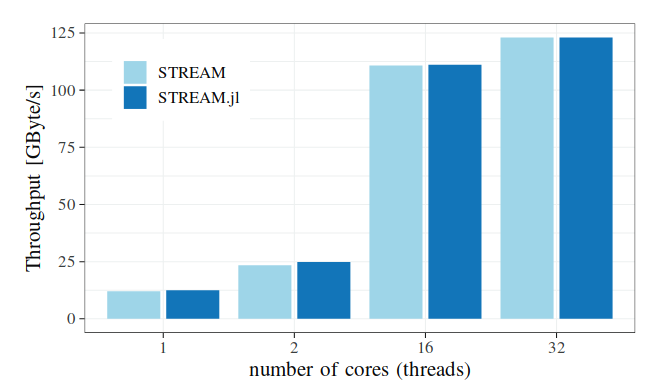
\includegraphics[width=10cm]{images/stream-1.png}
  \caption{Pengujian Pertama Menggunakan STREAM}
  \label{gambar stream-1}
  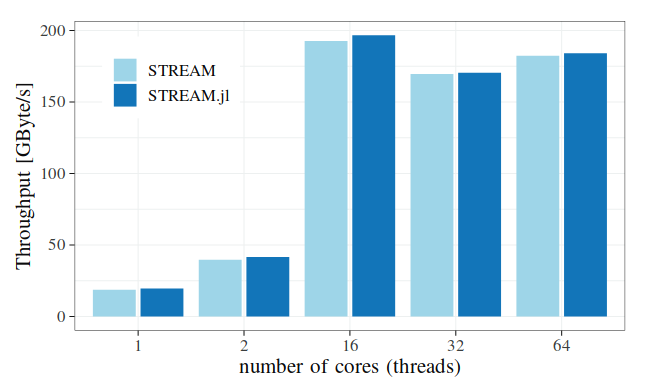
\includegraphics[width=10cm]{images/stream-2.png}
  \caption{Pengujian Kedua Menggunakan STREAM}
  \label{gambar stream-2}
\end{figure}

Penggunaan Julia pada sistem HPC (\emph{High Performance Computation}) perlu
diuji lebih lanjut. \cite{hunoldBenchmarkingJuliaCommunication2020} telah
melakukan penelitian penggunaan Julia pada sistem HPC.
\cite{hunoldBenchmarkingJuliaCommunication2020} menggunakan 2 metode pengukuran
HPC, yakni dengan STREAM yang mana dapat menjelaskan bagaimana performa sistem
untuk membaca/menulis pada \emph{Dynamic RAM} (DRAM), dan metode kedua adalah
dengan menggunakan ReproMPI yang mana menjelaskan bagaimana performa sistem
pada komunikasi data antar \emph{node}. Pada ReproMPI, terdapat 3 fungsi yang
digunakan, yakni \texttt{MPI\_Bcast}, \texttt{MPI\_Alltoall}, dan
\texttt{MPI\_Allreduce}. Hasil performa menggunakan Julia ini dibandingkan
dengan Bahasa C. Bahasa C ini memjadi acuan dikarenakan Bahasa C sudah terbukti
mampu untuk bekerja pada sistem HPC.

Pada Gambar \ref{gambar stream-1} dan \ref{gambar stream-2}, STREAM merupakan
simulasi yang ditulis dengan Bahasa C, sedangkan STREAM.jl merupakan simulasi
yang ditulis dengan Bahasa Julia. Dari kedua gambar tersebut, terlihat bahwa
Bahasa Julia mempunyai performa untuk membaca/menulis DRAM yang hampir seimbang
dengan Bahasa C.

\begin{figure}[H]
  \centering
  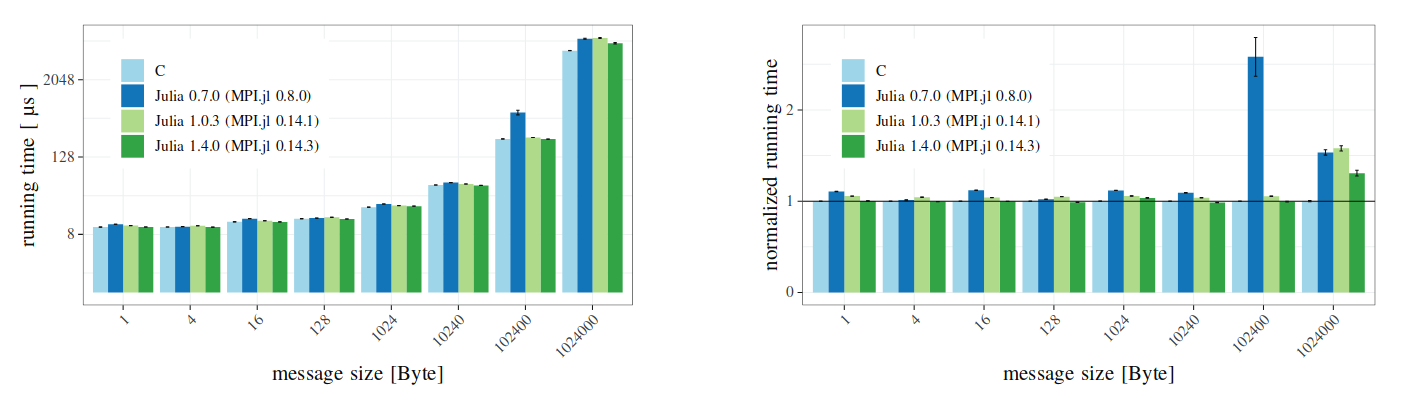
\includegraphics[width=14cm]{images/mpi-1.png}
  \caption{Pengujian Menggunakan MPI pada fungsi \texttt{MPI\_Bcast}}
  \label{gambar mpi-1 bcast}

  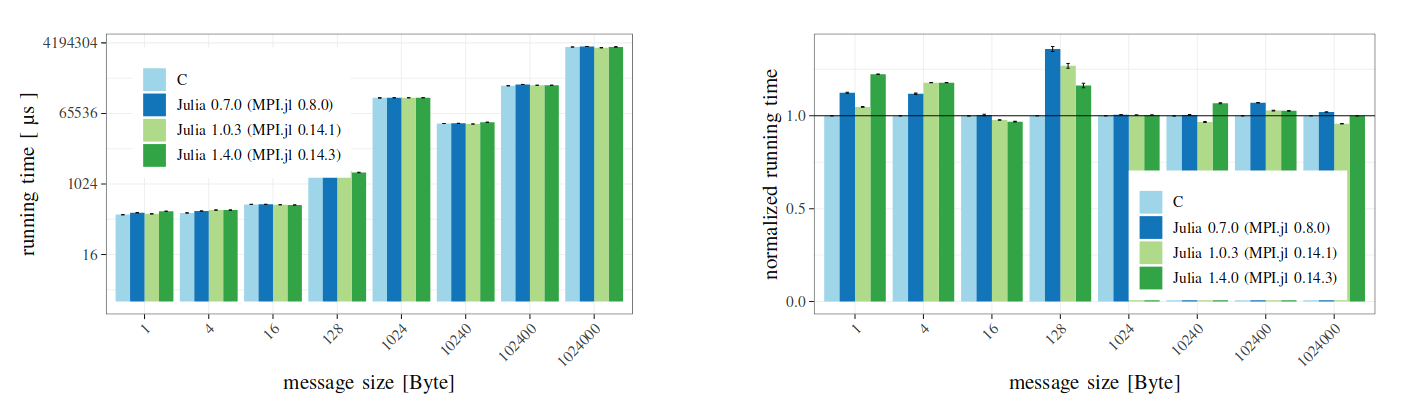
\includegraphics[width=14cm]{images/mpi-2.png}
  \caption{Pengujian Menggunakan MPI pada fungsi \texttt{MPI\_Alltoall}}
  \label{gambar mpi-2 alltoall}

  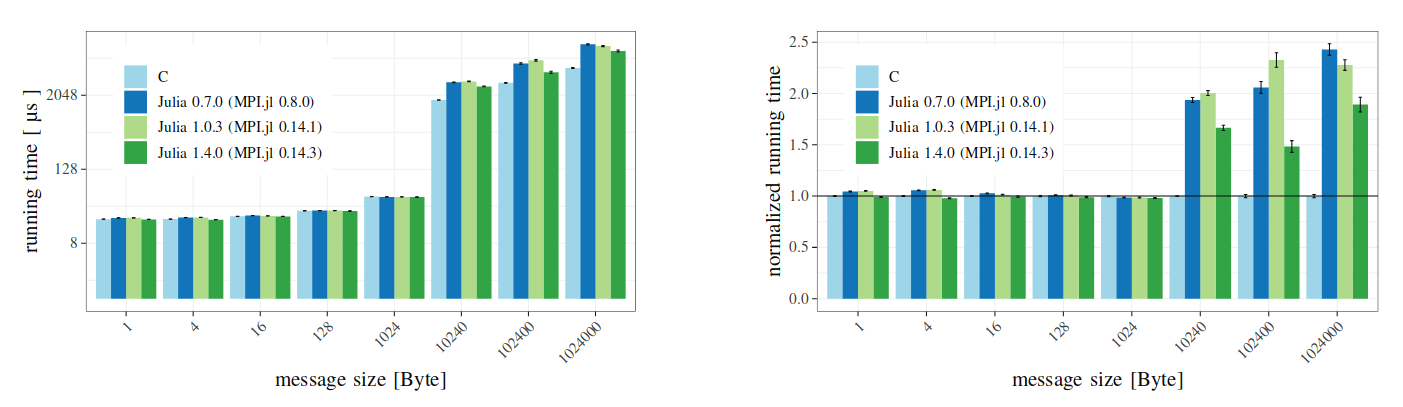
\includegraphics[width=14cm]{images/mpi-3.png}
  \caption{Pengujian Menggunakan MPI pada fungsi \texttt{MPI\_Allreduce}}
  \label{gambar mpi-3 allreduce}
\end{figure}

Pada Gambar \ref{gambar mpi-1 bcast}, \ref{gambar mpi-2 alltoall}, dan
\ref{gambar mpi-3 allreduce}, terlihat bahwa performa Bahasa Julia untuk
simulasi MPI umumnya memiliki nilai performa yang sama seperti Bahasa C.
Bahkan, sebenarnya untuk beberapa percobaan, performa Julia lebih baik daripada
C.

Dari kedua metode percobaan yang sudah dilakukan, dapat disimpulkan bahwa
performa Julia umumnya sama seperti C. Sehingga dapat dikatakan bahwa Julia
sudah bisa digunakan untuk sistem HPC.

\section{Pemrograman Julia dalam Komputasi Ilmiah}

Penggunaan Julia dalam komputasi ilmiah telah menjadi subjek penelitian yang
signifikan dalam beberapa tahun terakhir. Kemampuan Julia dalam menyeimbangkan
kinerja tinggi dan kemudahan pemrograman telah menjadikannya pilihan yang
menarik dalam berbagai bidang ilmiah. Berikut adalah tinjauan beberapa
literatur penting yang membahas aspek-aspek kunci dari penggunaan Julia dalam
komputasi ilmiah.

\cite{kulyabovComputerAlgebraJULIA2021} mengeksplorasi kemampuan Julia dalam aljabar
komputer. Hasil studi ini menunjukkan bagaimana Julia dapat digunakan untuk
komputasi simbolik dalam pemodelan matematis. \cite{kulyabovComputerAlgebraJULIA2021}
juga menyoroti bahwa Julia menawarkan sintaks yang sederhana dan kinerja yang memuaskan,
yang sangat bermanfaat dalam komputasi ilmiah. Kajian ini mendemonstrasikan kemampuan
Julia untuk mengintegrasikan komputasi numerik dan simbolik dalam satu kerangka kerja,
yang memungkinkan peneliti untuk melakukan analisis yang lebih kompleks dengan
efisiensi yang lebih tinggi.

\cite{tomasiNewSolutionsScientific2018} membahas fitur dan kekurangan Julia, serta
aplikasinya dalam astronomi dan astrofisika. Studi ini menekankan kecepatan
eksekusi yang tinggi dan ekspresifitas yang ditawarkan oleh Julia, yang mirip dengan
bahasa yang dikompilasi secara statis seperti C++ atau Fortran, sembari tetap
menyediakan shell interaktif dan dukungan penuh untuk Jupyter. Artikel ini membuktikan
bahwa Julia tidak hanya efisien dalam hal kinerja tetapi juga dalam hal produktivitas,
yang sangat penting dalam penelitian ilmiah.

\cite{zappanardelliJuliaSubtypingRational2018} memberikan definisi formal dari
relasi subtype dalam Julia dan memotivasi desainnya. Kajian ini penting karena menyoroti
bagaimana anotasi tipe pada deklarasi metode dalam Julia digunakan untuk memilih
metode yang paling tepat untuk sekumpulan argumen tertentu. Penelitian ini valid
secara empiris dengan implementasi definisi mereka yang dibandingkan dengan
implementasi Julia yang ada pada program dunia nyata. Temuan mereka menunjukkan keakuratan
dan efisiensi pendekatan subtyping Julia, yang sangat penting dalam pemrograman
multi-dispatch yang digunakan dalam komputasi ilmiah.

\cite{xiaoJuliaLanguageComputational2022b} melakukan survei komprehensif tentang
penggunaan bahasa Julia dalam mekanika komputasi. Penelitian ini menyoroti penggunaan
metode numerik dalam Julia dan menggambarkan bagaimana Julia memungkinkan peningkatan
abstraksi dan produktivitas. \cite{xiaoJuliaLanguageComputational2022b} membahas
kemampuan Julia dalam pengembangan paket perangkat lunak untuk mekanika
komputasi dan menantang penggunaan bahasa pemrograman yang lebih umum seperti
MATLAB atau Python dalam bidang ini. Studi ini menunjukkan bahwa Julia tidak hanya
efektif dalam hal kinerja tetapi juga dalam memberikan pendekatan yang lebih intuitif
untuk pemodelan dan simulasi dalam mekanika komputasi.

Kesimpulannya, Julia mempunyai kemampuan yang baik dalam komputasi ilmiah.
Julia menawarkan keseimbangan antara produktivitas dan kinerja. Dengan
kemampuan komputasi simbolik dan numeriknya, Julia tidak hanya meningkatkan
efisiensi dalam pemodelan dan analisis, tetapi juga mendukung inovasi dan
kemajuan dalam berbagai disiplin ilmiah.

% \section{Integrasi GPU dalam Fisika Komputasi}

% [Isinya berdasarkan metode]

% ==================================================

% \section{Komputasi Paralel dalam Fisika}

% \section{Perkembangan Terkini dalam GPU dan Julia}

% Penjelasan mengapa GPU lebih baik daripada CPU
% \section{Kinerja GPGPU}

% % Evolusi Pemrograman GPU:
% Komputasi GPU praktis dimulai dengan pengenalan CUDA (Compute Unified Device Architecture)
% oleh NVIDIA dan Stream oleh AMD, yang merupakan API (Application Programming
% Interface) yang dirancang untuk digunakan bersama dengan perangkat keras yang NVIDIA
% dan AMD sediakan. CUDA adalah sebuah platform dan model pemrograman yang
% memungkinkan para pengembang untuk menggunakan kekuatan komputasi GPU untuk
% proses yang lebih efisien dan canggih \citep{oanceaGPGPUComputing2014}.

% \begin{figure}[h]
%   \centering
%   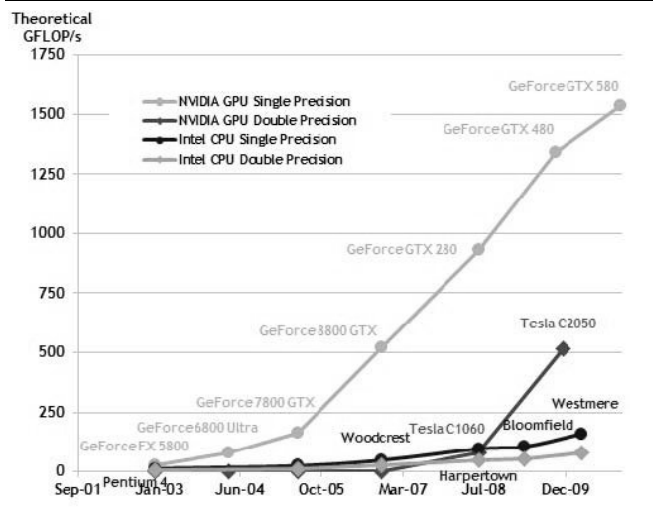
\includegraphics[width=10cm]{images/gpu-vs-cpu-flop-rates.png}
%   \caption{Tingkat FLOP teoritis dari GPU dan CPU}
%   \label{gambar flop rates gpu dan cpu}
% \end{figure}

% \cite{oanceaGPGPUComputing2014} menjelaskan bahwa \emph{flop rate} dari GPU dan CPU
% adalah seperti Gambar \ref{gambar flop rates gpu dan cpu}. Flop rate adalah
% ukuran kinerja yang menggambarkan seberapa cepat GPU dapat melakukan perhitungan
% matematika floating-point. Semakin tinggi flop rate, semakin cepat GPU dalam
% menyelesaikan operasi perhitungan yang kompleks. Terlihat pada Gambar \ref{gambar
% flop rates gpu dan cpu} bahwa perhitungan dengan menggunakan GPU mempunyai nilai
% teoritis flop rates yang jauh diatas CPU. Sehingga dapat disimpulkan bahwa GPU
% mempunyai kecepatan perhitungan kompleks yang jauh lebih tinggi daripada GPU.

% Sammy

% Pemelajaran mendalam (\emph{deep learning}) sebagai sebuah pemahaman telah lahir
% sejak tahun 1940an. Namun pemelajaran mendalam sebagai istilah yang tren memang
% baru muncul belakangan. Setidaknya ada tiga gelombang pengembangan pemelajaran mendalam
% yang ditandai dengan nomenklaturnya \citep{goodfellow_bengio_courville_2016}. Gelombang
% pertama (1940-1960an), istilah pemelajaran mendalam dikenal dengan \emph{cybernetics}
% yang merupakan pengembangan dari teori pola pemelajaran biologis \citep{mcculloch_pitts_1943, morris_1999}
% dan implementasi pertama pada model \emph{perceptron} \citep{rosenblatt_1958}.

% Pada gelombang kedua (1980-1995), dikenal dengan istilah \emph{connectionism}
% yang menggunakan pendekatan \emph{connectionist} dengan gebrakan baru yaitu perambatan
% mundur (\emph{back-propagation}) untuk melatih jaringan saraf (\emph{neural
% network}) dengan satu atau dua lapisan tersembunyi \citep{rumelhart_hinton_williams_1986}.
% Dan akhirnya gelombang ketiga atau masa kontemporer dimulai pada sekitar tahun 2006
% hingga sekarang yang dikenal dengan \emph{deep learning} \citep{hinton_osindero_teh_2006, NIPS2006_5da713a6}.

% Ilmu saraf memberikan wawasan yang banyak mengenai cara bekerja sebuah jaringan saraf
% biologis untuk dikembangkan ke dalam algoritma jaringan saraf buatan untuk belajar
% memecahkan beragam tugas yang berbeda \citep{goodfellow_bengio_courville_2016}. Salah
% satunya adalah penjelasan dari ilmuwan saraf bagaimana musang dapat belajar melihat
% dengan daerah pemrosesan pendengaran di otaknya jika otaknya diatur ulang untuk mengirimkan
% sinyal visual ke area tersebut \citep{von_melchner_pallas_sur_2000}. Hal ini kemudian
% menunjukkan bahwa mayoritas otak mamalia menggunakan algoritma tunggal untuk memecahkan
% kebanyakan tugas yang berbeda. Dari cara kerja tersebut, terinspirasilah ide utama
% untuk memiliki banyak unit komputasional yang menjadi pintar melalui interaksi dengan
% unit lain \citep{goodfellow_bengio_courville_2016}.

% Neocognitron \citep{fukushima_1980} memperkenalkan model arsitektur yang sangat bagus
% untuk memroses gambar yang terinspirasi dari sistem visual mamalia dan yang kemudian
% menjadi cikal bakal ide untuk pengembangan jaringan saraf konvolusi modern (\emph{modern
% convolutional neural network} \citep{726791, lecun_kavukcuoglu_farabet_2010}.

% Penyelesaian persamaan diferensial parsial menggunakan metode jaringan saraf
% buatan dimulai sejak tahun 1990an yang dimulai oleh \cite{lee_kang_1990} dengan
% artikelnya yang berjudul '\emph{Neural algorithm for solving differential
% equation}' yang terbit di \emph{Journal of Computational Physics}. Kemudian pada
% dekade yang sama muncul beberapa artikel yang membahas tentang topik ini, yaitu
% oleh Dissanayake dan Phan-Tien pada tahun 1994 dan Lagaris, dkk. pada tahun
% 1998.

% Dalam \citep{lagaris1998}, solusi persamaan diferensial dalam koordinat kartesian
% yang coba diselesaikan merupakan penjumlahan dari dua bagian. Bagian yang
% pertama merupakan permasalahan syarat batas atau syarat awal dan mengandung
% parameter yang tidak dapat diubah-ubah. Dan bagian yang kedua adalah bagian yang
% tidak memiliki hubungan dengan bagian syarat awal/syarat batas dan mengandung perambatan
% maju dari jaringan saraf buatan. Pengaplikasian metode ini dapat digunakan pada
% persamaan diferensial biasa tunggal, persamaan diferensial biasa berpasangan,
% dan persamaan diferensial parsial. Metode ini dikomparasikan dengan solusi dari metode
% numerik Galerkin \emph{finite element}.

% Usaha-usaha awal penggunaan jaringan saraf buatan pada penyelesaian persamaan
% diferensial parsial ini sangat memanfaatkan algoritma perambatan mundur karena
% memberikan metode yang sangat akurat untuk menghitung ralat. Namun usaha-usaha ini
% memiliki kendala yang kurang lebih sama, yaitu hanya mampu menangani fungsi ruas
% kanan dan syarat batas tertentu saja.

% Dengan perkembangan kekuatan komputasi pada tahun 2000an, dimungkinkan untuk membuat
% model yang lebih rumit, dan parameter yang lebih banyak, serta jumlah lapisan (\emph{layer})
% yang lebih banyak. \cite{Smaoui2004} menggunakan jumlah daya komputasional yang lebih
% besar untuk menginvestigasi model yang lebih mendalam. menggunakan \emph{multilayer
% perceptron} untuk memprediksi dinamika dari dua persamaan diferensial parsial nonlinear
% menggunakan dekomposisi Kahunen-Loeve dan jaringan saraf buatan.
% \cite{baymani2010} mengembangkan jaringan saraf buatan untuk penyelesaian
% permasalahan Stokes. Permasalahan Stokes campuran ditransformasi ke dalam tiga permasalahan
% Poisson koordinat kartesian yang kemudian diselesaikan untuk mendapatkan hasil dari
% permasalahan Stokes tersebut. Hasil yang didapat dari metode jaringan saraf
% buatan ini kemudian dikomparasikan dengan metode numerik dari penelitian lainnya
% dan hasil eksaknya. Dari penelitian tersebut didapatkan bahwa pendekatan jaringan
% saraf tiruan yang baru memberikan hasil yang memiliki akurasi yang lebih tinggi dan
% jumlah parameter yang digunakan lebih sedikit dari model konvensional.

% \cite{DBLP:journals/corr/abs-1711-10561} memperkenalkan jaringan saraf terinformasi
% fisika (\emph{physics informed neural networks} (PINN)), yaitu jaringan saraf yang
% dilatih untuk menyelesaikan tugas-tugas pembelajaran yang diawasi dengan tetap memperhatikan
% hukum fisika tertentu yang dijelaskan oleh persamaan diferensial parsial nonlinier
% umum. Pengembangan tersebut berada pada koridor untuk memecahkan dua masalah
% utama yaitu solusi berbasis data dan penemuan berbasis data dari persamaan
% diferensial parsial.

% Seiring dengan perkembangan model \emph{deep learning}, suatu terobosan dalam
% penyelesaian persamaan diferensial parsial menggunakan jaringan saraf buatan
% kemudian ditemukan. Para peneliti kemudian mengembangkan model jaringan saraf buatan
% konvolusi (\emph{convolutional neural network}/ CNN) dengan hipotesis bahwa dengan
% menggunakan CNN, parameter yang digunakan akan lebih sedikit sehingga akan
% banyak melakukan penghematan sumber daya komputer serta akan memberikan hasil
% yang lebih akurat. Selain itu, menurut \cite{Li_Li_Gao}, CNN memiliki kemampuan yang
% lebih baik untuk mengenali masukan gambar.

% \cite{shan_2020_study} mengembangkan model penyelesaian persamaan Poisson menggunakan
% CNN untuk memprediksi potensial listrik dengan variasi pada eksitasi dan distribusi
% permitivitas pada bidang kartesian 2 dimensi dan 3 dimensi. Penelitian ini
% menggunakan desain \emph{cost function} yang dikustomisasi dan data yang didapat
% dari metode numerik beda-hingga. Model yang dikembangkan dapat melakukan peforma
% yang cukup efektif dibandingkan dengan metode numerik yang digunakan untuk
% membentuk data latih, dengan rata-rata ralat prediksi kurang dari 3\%.

% Perkembangan yang cukup signifikan dilakukan oleh \cite{Ozbay2021} dengan
% mengembangkan arsitektur CNN untuk menyelesaikan persamaan Poisson 2 dimensi
% pada koordinat kartesian dengan variasi resolusi yang diberikan oleh ruas kanan
% persamaan, sembarang syarat batas, dan variasi parameter grid. Permasalahan syarat
% batas diselesaikan dengan metode baru, mendekomposisikan persaman Poisson yang
% asli ke dalam satu persamaan Poisson homogen dan empat submasalah Laplace
% nonhomogen. Model yang dikembangkan terbukti dapat mengungguli model dengan jaringan
% saraf tiruan konvensional dan dapat memprediksi dengan rata-rata presentase ralat
% di bawah 10\%.

% \cite{cheng2021using} menyelesaikan persamaan Poisson 2 dimensi dengan syarat
% batas Dirichlet nol menggunakan lapisan konvolusi secara penuh dengan arsitektur
% U-Net \citep{DBLP:journals/corr/RonnebergerFB15} yang didefinisikan dengan variasi
% pada jumlah percabangan, kedalaman, dan medan reseptif. Pada penelitian tersebut
% didapati bahwa medan reseptif memiliki peran yang penting dalam menangkap
% struktur topologis dari masukan pada tiap lapisan. Untuk menghitung syarat batas
% dan interior, digunakan dua syarat batas, yaitu \emph{dichlet loss} dan \emph{inside
% loss} serta syarat batas alternatif yaitu \emph{laplacian loss}. Untuk pelatihan
% digunakan dataset dengan distribusi muatan acak dan dataset dengan dengan distribusi
% mengikuti aturan deret Fourier.

% Sebagai domain fisis, dalam penelitian ini akan digunakan model pendorong Hall (\emph{Hall
% thruster}) sebagai perwakilan masalah fisis perhitungan potensial listrik di koordinat
% silinder. \cite{braga_miranda_2019} dari Laboratorium Fisika Plasma Universitas
% Brasil (LFP-UnB) sejak 2004 sedang mengembangkan pendorong Hall yang disebut
% PHall yang memiliki perbedaan dalam dimensi kanal, parameter operasi, dan
% mekanisme pembentukan medan magnet yang dibutuhkan dengan SPT-100. SPT-100
% dijadikan sebagai patokan dan pembanding dalam pembangunannya. Model 2 dimensi,
% spesifikasi serta, gambaran simulasi tentang SPT-100 dijelaskan dalam karya mereka.

% Penelitian ini akan memecahkan masalah persamaan diferensial parsial berupa persamaan
% Poisson yang diterapkan pada domain fisis pedorong Hall SPT-100 pada koordinat silinder
% dua dimensi menggunakan metode jaringan saraf konvolusi dengan \emph{ground
% truth} yang dihitung menggunakan metode numerik Gauss-Seidel.
  \chapter{DASAR TEORI}

\section{Pengantar GPU dan \emph{General Purpose GPU} (GPGPU)}

\subsection{Sejarah dan perkembangan GPU}

% #### Awal Mula dan Evolusi Awal

Dalam sejarahnya, \emph{Graphics Processing Unit} (GPU) awalnya dirancang untuk
mempercepat pemrosesan gambar pada komputer. Pemrosesan gambar yang memerlukan
GPU pada awalnya hanya dibutuhkan untuk permainan video game. Pada tahun
1970-an hingga 1980-an, beberapa perangkat yang mengadopsi sistem paralel
seperti GPU diantara nya adalah Atari 2600 dan ARTC HD63484
\citep{wikipediaGraphicsProcessingUnit2023}.

Perkembangan GPU untuk komputer pribadi dimulai pada tahun 1980-an. Pada awal
tahun tersebut, terdapat produk NEC µPD7220 yang menjadi implementasi pertama
dari GPU yang dapat digunakan pada komputer pribadi. Produk NEC µPD7220 ini
mempunyai harga terjangkau dan kualitas grafis yang tinggi, sehingga membuat
GPU ini terkenal hingga pertengahan tahun 1980-an. Pada tahun 1985, muncul
produk baru bernama Amiga dengan menggunakan kustom chip grafis. Amiga ini
dapat digunakan untuk menggambar garis, memanipulasi bitmap, dan melakukan
isian warna pada suatu area \citep{wikipediaGraphicsProcessingUnit2023}.

Dalam perkembangannya, NVIDIA memperkenalkan GPU pertama mereka yang bernama
NVIDIA GeForce 256. GPU ini mampu melakukan pemrosesan grafis secara
\emph{real-time}, dan mampu melakukan banyak perhitungan floating-point dari
tahan shading vertex hingga tahap shading fragment. NVIDIA GeForce 256 juga
memiliki bandwidth memori yang tinggi
\citep{dallyEvolutionGraphicsProcessing2021}. Pada tahun berikutnya, NVIDIA
memperkenalkan NVIDIA GeForce 8 dengan unit pemrosesan stream generik yang
baru. NVIDIA GeForce 8 menunjukkan kemajuan performa komputasi yang jauh lebih
baik daripada CPU. Dari perbedaan performa inilah kemudian para peneliti
menemukan cara untuk mengubah shader vertex dan shader fragment, menjadi suatu
data yang dapat diolah oleh GPU secara paralel. Proses penggunaan GPU untuk
melakukan komputasi umum secara paralel disebut dengan \emph{General Purpose
	GPU} atau GPGPU. Beberapa bidang yang menggunakan GPGPU ini diantara lain
adalah bidang pembelajaran mesin, eksplorasi minyak, aljabar linear, statistik,
rekonstruksi 3D, dan penetapan harga opsi saham
\citep{wikipediaGraphicsProcessingUnit2023}.

Pada perkembangannya, GPU telah mengalami perubahan bentuk ukuran, daya,
kinerja, dan harga. Hal ini membuat GPU membukakan jalan bagi inovasi lebih
lanjut di berbagai bidang. Dari yang awalnya hanya digunakan untuk bermain
video game saja, menjadi komponen yang diperlukan di smartphone, \emph{virtual
	reality}, pembelajaran mesin, mobil tanpa pengemudi, pesawat ruang angkasa,
robot, perangkat rumah pintar, dan banyak bidang lainnya
\citep{businesswireHistoryGPUInception2023}.

\subsection{Transisi GPU dari pemrosesan grafis ke GPGPU}

% #### Kemajuan Teknologi dan Penemuan GPGPU
Perkembangan GPGPU menjadi lebih praktis dan populer setelah tahun 2001, dengan
munculnya shader yang dapat diprogram dan mendukung \emph{floating point} pada
prosesor grafis. Masalah yang melibatkan vektor dan matriks yang mempunyai
n-dimensi dapat dengan mudah diterjemahkan dan diproses oleh GPU. Pada tahun
2003, ditemukan pendekatan berbasis GPU untuk solusi masalah aljabar linear
umum. Pendekatan pada GPU ini berjalan lebih cepat daripada pendekatan yang
menggunakan CPU. Perbedaan kecepatan ini merupakan tonggak awal GPGPU menjadi
banyak digunakan untuk masalah komputasi umum
\citep{wikipediaGeneralpurposeComputingGraphics2023}.
\cite{pharrGPUGemsProgramming2005} menyatakan bahwa pada bidang ilmu komputer
dan visualisasi, GPGPU juga menunjukkan hasil yang baik. Hasil yang baik ini
dapat dicapai dengan menerapkan GPU pada masalah komputasi data-paralel.

% #### Arsitektur GPU dan Pemrograman GPGPU
Memaksimalkan kinerja dari GPU memerlukan pemahaman tentang arsitekturnya. GPU
dirancang untuk grafis komputer yang memiliki gaya komputasi paralel tinggi dan
menghasilkan output piksel berwarna dari elemen data yang independen. Desain
ini adalah kunci saat memprogram GPU, baik untuk grafis maupun komputasi umum.
Pemrograman GPU untuk masalah komputasi umum awalnya tertanam dalam API
(\emph{Application Programming Interface}) dan bahasa pemrograman grafis
komputer. Dalam perkembangannya, API dan bahasa pemrograman grafis
disederhanakan, dimana menghasilkan API seperti CUDA dari NVIDIA, DirectCompute
dari Microsoft, dan OpenCL dari Apple/Khronos Group. API tersebut memungkinkan
penggunaan GPU tanpa memerlukan konversi data eksplisit ke bentuk grafis
\citep{pharrGPUGemsProgramming2005}.

% #### Kasus Penggunaan dan Contoh Aplikasi
Aplikasi yang mendapat manfaat paling besar dari pemrosesan GPU adalah aplikasi
yang memiliki intensitas aritmatika yang tinggi, seperti solusi sistem
persamaan linear dan simulasi berbasis fisika. Contoh lain nya adalah simulasi
aliran dengan batasan kompleks dan algoritma jarak terpendek untuk semua
pasangan, seperti yang digunakan dalam prediksi struktur protein. Jenis
komputasi ini berkinerja baik pada GPU karena sifatnya yang sangat
data-paralel: mereka terdiri dari aliran besar elemen data, di mana kernel
komputasi yang identik diterapkan \citep{pharrGPUGemsProgramming2005}.

\subsection{Arsitektur dan karakteristik GPU}

% 2. Arsitektur GPU: Perbandingan dengan CPU

\begin{figure}[H]
	\centering
	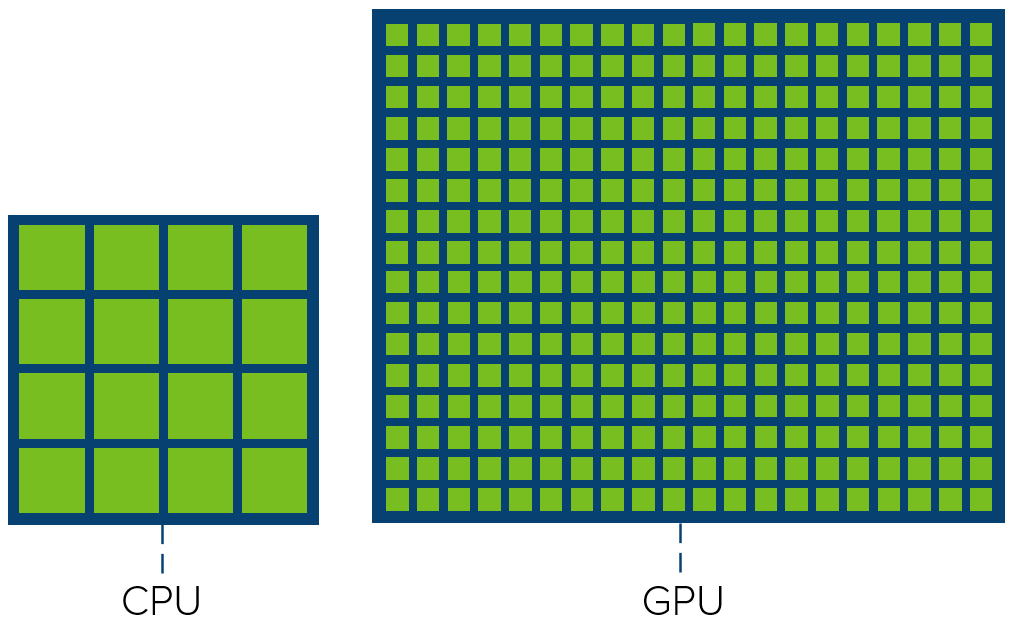
\includegraphics[width=10cm]{images/cpu-vs-gpu-cores.png}
	\caption{Jumlah Inti CPU dan Inti GPU}
	\label{gambar gpu-cpu cores}
\end{figure}

Secara arsitektur, GPU memiliki arsitektur yang hampir sama dengan CPU. Namun
CPU berfokus pada kecepatan akses memori cache. Sedangkan GPU dirancang untuk
melakukan komputasi data secara paralel, sehingga dibutuhkan sebanyak mungkin
inti yang tersedia, seperti yang terlihat pada Gambar \ref{gambar gpu-cpu cores}.
Arsitektur yang digunakan oleh GPU biasanya disebut dengan arsitektur
stream SIMD (\emph{Single Instruction Multiple Data}) yang mana memanfaatkan
banyak inti dengan pemrosesan ringan \citep{helenGPUArchitectureStructure2020}.

% 4. Fitur Arsitektural Utama dan Implikasinya

% Fitur arsitektural utama GPU mencakup penggunaan inti pemrosesan yang banyak dan
% ringan, yang berbeda dari CPU yang menggunakan inti yang lebih sedikit tetapi lebih
% kuat. Implikasi dari arsitektur ini terhadap pembuatan program untuk GPGPU
% melibatkan pertimbangan khusus dalam hal bagaimana data dan tugas-tugas
% diorganisir dan dijalankan, serta jenis perangkat lunak yang paling sesuai untuk
% perangkat ini.

% 3. Model Komputasi Streaming dan 'Gap' Memori

Salah satu faktor penting dalam evolusi GPU adalah '\emph{gap}' memori, yaitu
perbedaan antara kecepatan komputasi terhadap kecepatan akses memori. Model
komputasi '\emph{streaming}' merupakan pendekatan yang paling cocok untuk GPU
modern. Ini dikarenakan model ini mempunyai efisiensi yang tinggi dalam
pemrosesan paralel \citep{pharrGPUGemsProgramming2005}.

% 5. GPU dalam High Performance Computing (HPC)

Dalam konteks High Performance Computing, GPU kini menjadi pilihan utama untuk
mempercepat beban kerja komputasi. Penggunaan GPGPU telah meluas ke berbagai
bidang, termasuk pemodelan 3D, infrastruktur VDI, dan lebih lanjut, menunjukkan
fleksibilitas dan kekuatan GPU dalam berbagai skenario komputasi
\citep{hagoortExploringGPUArchitecture2023}.

\begin{figure}[H]
	\centering
	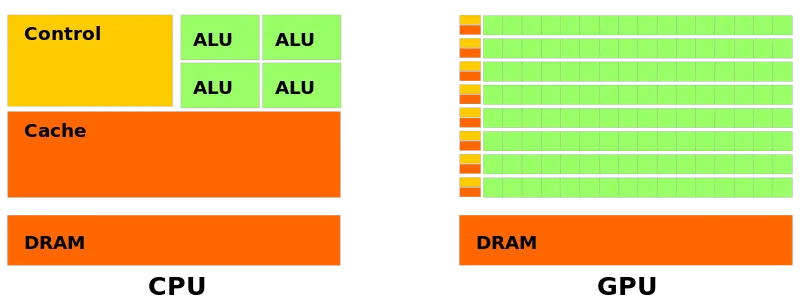
\includegraphics[width=14cm]{images/cpu-gpu-architecture.png}
	\caption{Arsitektur CPU dan GPU}
	\label{gambar gpu-cpu architecture}
\end{figure}

Berdasarkan \cite{learningUnderstandingArchitectureGPU2023}, arsitektur CPU dan
GPU dapat digambarkan skema nya seperti pada Gambar \ref{gambar gpu-cpu
	architecture}. Warna hijau menggambarkan unit komputasi atau \emph{cores}
(inti), warna orange menggambarkan memori, dan warna kuning menggambarkan unit
kontrol.

\subsubsection{Unit Komputasi}
\label{unit komputasi}

Pada Gambar \ref{gambar gpu-cpu architecture}, terlihat bahwa inti dari CPU
mempunyai ukuran yang lebih besar dari pada inti GPU. Beda ukuran ini
menggambarkan bahwa inti CPU mempunyai kecerdasan yang lebih tinggi daripada
inti GPU. Ini berarti inti CPU mampu mengatasi berbagai macam tugas kompleks
yang diperlukan oleh komputer. Pada Gambar \ref{gambar gpu-cpu architecture}
terlihat juga bahwa inti dari CPU mempunyai jumlah yang jauh lebih sedikit dari
pada GPU. Perbedaan ini dikarenakan memang GPU memiliki inti dengan jumlah yang
jauh lebih banyak daripada CPU.

Seiring berjalan nya waktu, inti CPU mempunyai evolusi yang semakin baik dalam
segi performa. Sebaliknya, inti GPU mempunyai perubahan yang semakin menurun.
Penurunan inti GPU ini bertujuan agar penggunaan inti GPU dapat mengkonsumsi
daya yang lebih rendah. Sehingga GPU akan bisa digunakan di berbagai perangkat,
termasuk perangkat mobile.

Dalam eksekusi nya, CPU menggunakan konsep \emph{out of order execution} (OOE),
yang mana instruksi pada CPU dapat segera diproses setelah sumber daya yang
diperlukan tersedia. Instruksi yang dijalankan inipun tidak perlu menunggu
instruksi sebelumnya selesai. Model eksekusi ini bertujuan untuk meningkatkan
pemanfaatan sumber daya dan mengurangi waktu tunggu eksekusi.

Berbeda dengan CPU, GPU tidak menggunakan konsep OOE, dan hanya menjalankan
instruksi saja. Tidak menggunakan OOE ini bertujuan untuk tetap menyederhanakan
arsitektur unit komputasi pada GPU. Selain itu, GPU memang didesain untuk
mengatasi tugas yang tidak kompleks. Pada dasarnya, semua tugas yang
menggunakan GPU hanya menggunakan operasi penjumlahan dan perkalian.

Operasi penjumlahan dan perkalian pada GPU secara umum menggunakan dua metode,
yakni \emph{Multiply-Add} (MAD) dan \emph{Fused Multiply-Add} (FMA). Pada
Gambar \ref{gambar mad-and-fma}, terlihat bahwa perbedaan utama antara MAD dan
FMA adalah ada di proses nya. Proses perkalian dan penjumlahan MAD dilakukan
secara berurutan yang mana menyebabkan ketelitian dari hasilnya akan berkurang.
Sedangkan pada FMA, setelah proses perkalian dan penjumlahan dilakukan
sekaligus yang menyebabkan hasilnya memiliki ketelitian yang tinggi. Dalam
kinerja nya, operasi FMA memungkinkan GPU untuk dapat meningkatkan kinerja yang
signifikan. Namun pada implementasi nya, operasi FMA memerlukan hardware khusus
untuk optimalisasi, sedangkan MAD bisa lebih umum dan tidak spesifik pada
perangkat keras tertentu.

\begin{figure}[H]
	\centering
	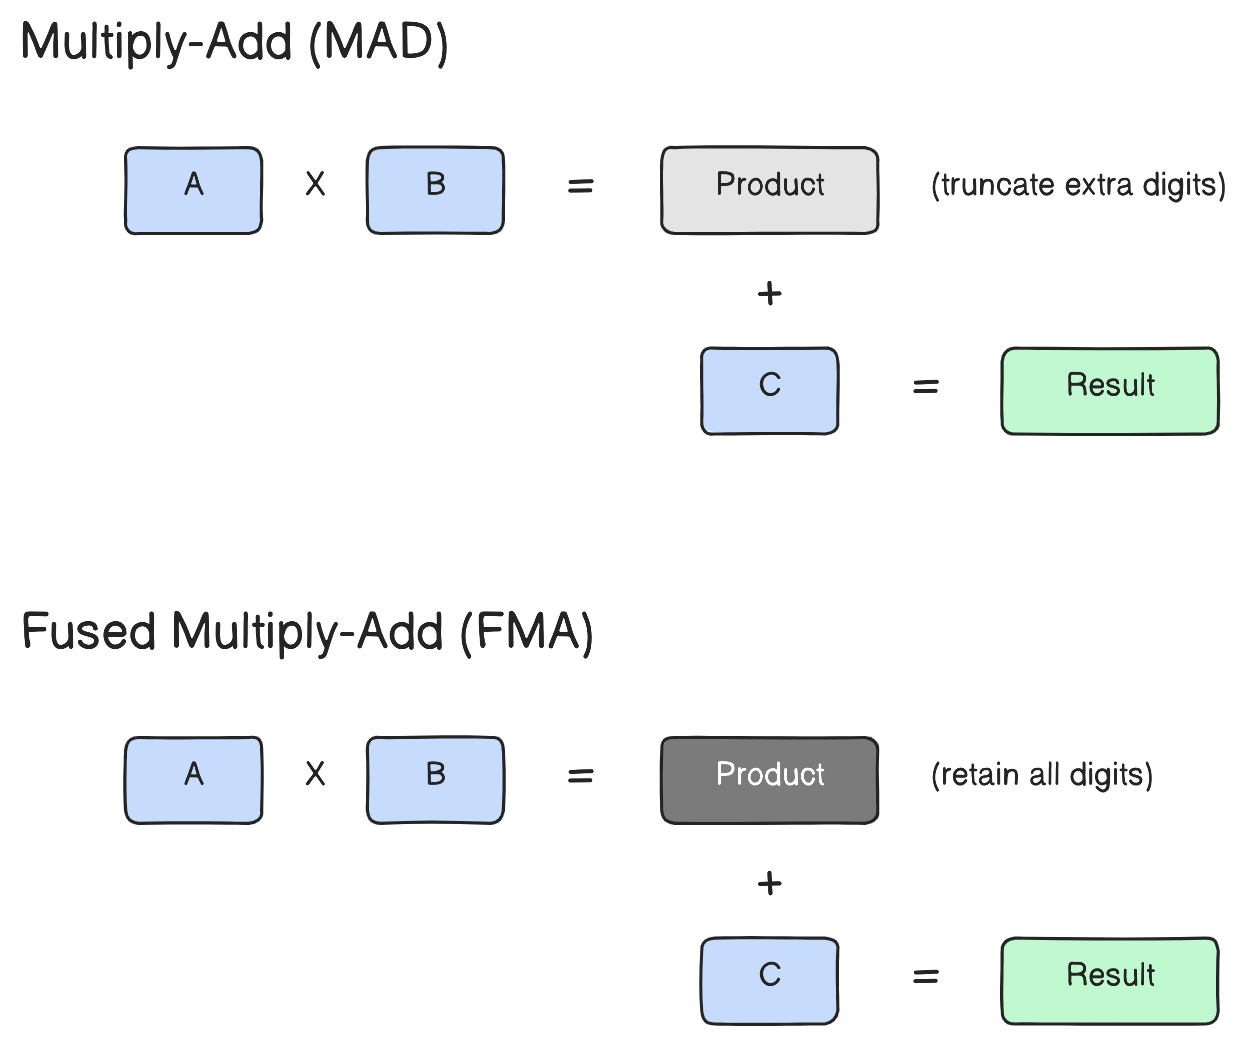
\includegraphics[width=10cm]{images/mad-and-fma-2.png}
	\caption{MAD dan FMA pada operasi GPU}
	\label{gambar mad-and-fma}
\end{figure}

Meskipun GPU terlihat hanya bisa melakukan operasi sederhana, namun operasi
sederhana ini dapat berupa operasi penjumlahan dan perkalian yang kompleks yang
mana bisa membentuk operasi pada tensor dan operasi pada \emph{ray-tracing}
seperti yang terlihat pada Gambar \ref{gambar ray tracing technique}. Kemampuan
utama GPU dalam menghasilkan \emph{render} yang bagus seperti pada Gambar
\ref{gambar ray tracing technique} pada dasarnya terletak pada kemampuan GPU
untuk melakukan operasi secara paralel. Dalam melakukan operasi secara paralel
ini, GPU menggunakan model \emph{Single Instruction Multiple Data} (SIMD) di
mana semua inti nya semua core menjalankan operasi yang sama pada data yang
berbeda.

\begin{figure}[H]
	\centering
	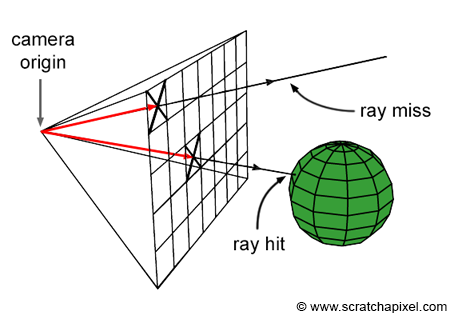
\includegraphics[width=5cm]{images/rt-setup2.png}
	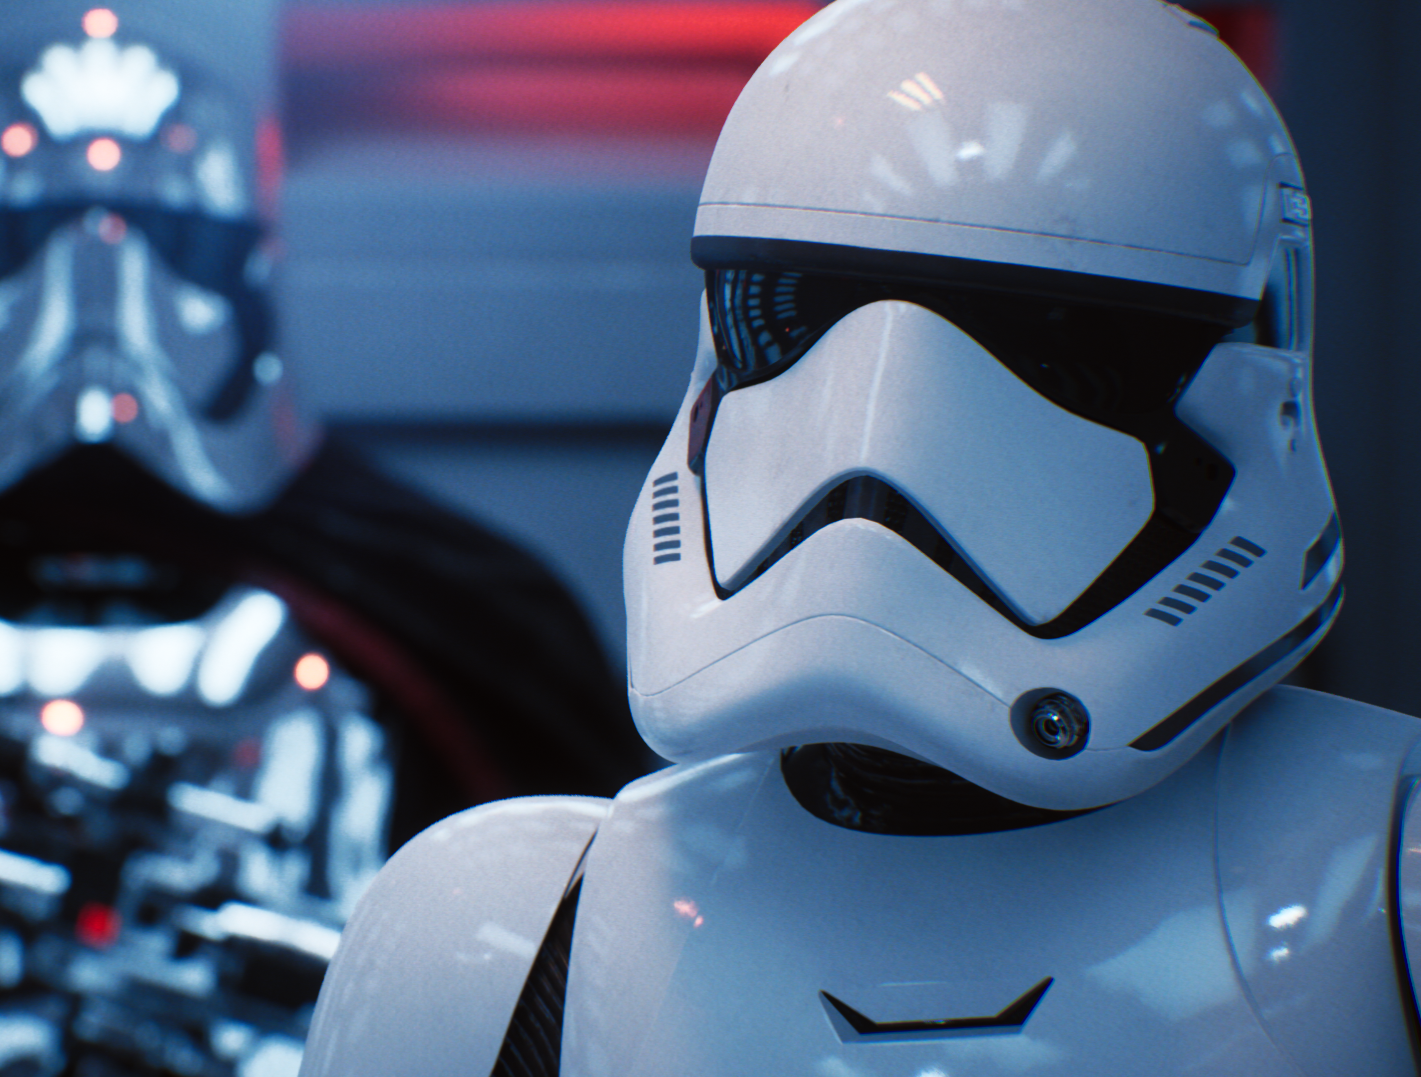
\includegraphics[width=5cm]{images/Reflections_02.png}
	\caption{Teknik \emph{Ray Tracing} dan Hasil \emph{Render} dengan menggunakan
		Teknik \emph{Ray Tracing}}
	\label{gambar ray tracing technique}
\end{figure}

\subsubsection{Memori}

Perbedaan model memori pada CPU dan GPU telah terlihat pada Gambar \ref{gambar
	gpu-cpu architecture} dengan blok yang berwarna orange. Sistem memori CPU
menggunakan \emph{Dynamic Random Access Memory} (DRAM) dengan ukuran yang
bervariasi. Komputer pribadi biasanya mempunyai ukuran DRAM berkisar 4GB hingga
128GB.

Komponen kunci lainnya dari memori CPU adalah \emph{cache}, yang mana memiliki
tujuan untuk mempercepat waktu akses antara CPU ke DRAM. Kecepatan akses ini
disebabkan karena letak CPU yang sangat dekat dengan \emph{cache}. \emph{Cache}
ini memiliki ukuran yang cukup kecil, biasanya berkisar puluhan KB per inti
CPU. \emph{Cache} umumnya terdiri dari tiga level, yakni Level 1 (L1), Level 2
(L2), dan Level 3 (L3). L1 memiliki letak paling dekat dengan CPU namun
memiliki ruang penyimpanan yang paling kecil (biasanya berkisar 64KB inti),
sedangkan L3 memiliki letak yang paling jauh dengan CPU namun memiliki ruang
penyimpanan yang paling besar daripada \emph{cache} lainnya (biasanya berkisar
4MB per inti). Proses CPU untuk mengambil data dari memori mempunyai urutan:
pencarian pada L1, pencarian pada L2, pencarian pada L3, pencarian pada DRAM.

Sementara itu, GPU menggunakan memori yang bertipe DRAM juga yang disebut
dengan \emph{Global Memory} atau GMEM. Ukuran GMEM ini biasanya lebih kecil
dibandingkan DRAM pada CPU. GMEM biasanya memiliki ukuran yang berkisar 2GB
pada kartu grafis (GPU) ekonomis, hingga ukuran 40GB atau 80GB pada kartu
grafis yang lebih mahal.

% \section{Pemrograman GPU}
% \subsection{Dasar-dasar pemrograman GPU}
% \subsection{Perbandingan antara pemrograman CPU dan GPU}
% \subsection{Alat dan teknologi yang digunakan dalam pemrograman GPU}

\section{Bahasa Pemrograman Julia}

Bahasa Julia dirilis pada tahun 2012 dan telah diterima secara luas di kalangan
data scientist dan para penggiat matematika. Bahasa ini diciptakan karena
adanya kebutuhan akan bahasa pemrograman yang ideal untuk pengkodean aritmatika
\citep{ismiPentingUntukData2021}. Tujuan utama Julia adalah mengkombinasikan
kemudahan dalam penggunaan, kecepatan, dan efisiensi dalam satu bahasa
pemrograman. Julia memiliki sifat pengetikan opsional, mengadopsi berbagai
bahasa pemrograman. Sehingga, dalam efisiensi dan kecepatan dan efisiensi
sistem tingkat rendah, Julia dapat bersaing dengan pemrograman seperti C atau
C++. Kemudian, dalam kemudahan penggunaan, Julia memiliki syntax yang mudah
dipahami seperti halnya bahasa pemrograman Python. Pada bagian ini akan
dijelaskan secara singkat mengenai sintaks - sintaks dasar Julia beserta
perbandingan nya dengan Bahasa Python. Penulis menggunakan
\cite{dokumentasijuliaJuliaDocumentationJulia2024} untuk menulis sintaks Julia,
dan menggunakan buku dari \cite{matthesPythonCrashCourse2016} untuk menulis
sintaks Python.

\subsection{Variable dan Tipe Data}

Variabel dalam Julia dibuat dengan cara menetapkan nilai pada suatu nama
menggunakan \emph{assignment operator} "\cw{=}". Sintaks ini cukup identik
dengan bahasa Python. Berikut merupakan contoh penulisan variable Julia dan
Python

\begin{lstlisting}
# Julia
my_name = "Alfarizi"
my_favourite_number = 42
my_favourite_pie = 3.1415

# Python
my_name = "Alfarizi"
my_favourite_number = 42
my_favourite_pie = 3.1415
\end{lstlisting}

\noindent
Sama seperti Python, Julia merupakan bahasa yang bertipe dinamis, yang berarti tidak memerlukan deklarasi
tipe variabel secara eksplisit. Tipe dari variabel secara otomatis diperoleh
berdasarkan tipe datau \emph{value} nya. Selain itu, variabel dalam Julia dapat mengubah
tipenya selama runtime. Misalnya saja seperti kode berikut:

\begin{lstlisting}
x = 20    # x adalah integer
x = "abc" # x berubah menjadi string
\end{lstlisting}

\label{basic tipe data julia} Dalam menyimpan suatu data, Julia mendukung
beberapa tipe data dasar seperti pada tipe data bahasa pemrograman pada umumnya.
Berikut merupakan tipe data dasar yang dimiliki oleh Julia:

\begin{itemize}
	\item \textbf{Angka}: Ini termasuk beberapa subjenis seperti:
	      \begin{itemize}
		      \item Bilangan bulat (\cw{Int8}, \cw{Int16}, \cw{Int32}, \cw{Int64}, \cw{Int128})

		      \item Angka floating-point (\cw{Float16}, \cw{Float32}, \cw{Float64})

		      \item Angka kompleks (\cw{ComplexF32}, \cw{ComplexF64})
	      \end{itemize}

	\item \textbf{Boolean}: \cw{Bool} mewakili nilai Boolean \cw{true} dan \cw{false}.

	\item \textbf{Karakter} dan \textbf{String}:
	      \begin{itemize}
		      \item Karakter: \cw{Char} digunakan untuk karakter Unicode tunggal.

		      \item String: \cw{String} mewakili rangkaian karakter.
	      \end{itemize}

	\item \textbf{Array}: \cw{Array{T,N}} menandakan array multidimensi dari
	      elemen tipe T.

	\item \textbf{Tuple}: \cw{Tuple{T1,T2,...}} menunjukkan koleksi terurut dari
	      elemen dengan tipe berbeda T1, T2, dan lain-lain.

	\item \textbf{Dictionaries}: \cw{Dict{K,V}} mewakili kumpulan pasangan kunci-nilai
	      di mana K dan V adalah tipe kunci dan nilai.
\end{itemize}

Dalam penamaan, nama variabel dalam Julia dapat mencakup subset simbol Unicode,
yang memungkinkan berbagai macam kemungkinan penamaan, termasuk penggunaan
simbol seperti huruf Yunani. Misalnya, untuk mewakili variabel dengan huruf
Yunani dalam sebagian besar lingkungan pengembangan Julia, Anda dapat
menggunakan sintaks seperti LaTeX (misalnya, \cw{\alpha} untuk $\alpha$).
Sintaks ini juga mencakup penambahan subskrip, superskrip, dan lain-lain.

% \markdownInput{markdowns/variable-dan-tipe-data.md}

% Melakukan variable

% \begin{lstlisting}[caption={Deklarasi variable}]{language=julia}
% my_name = "Aurelio"
% my_favourite_number = 42
% my_favourite_pie = 3.1415
% \end{lstlisting}

\subsection{Deklarasi Fungsi}

Fungsi merupakan deretan perintah yang dijalankan secara berurutan. Sama
seperti pada Matematika, fungsi digunakan untuk menyederhanakan deretan
perintah yang kemungkinan nanti nya akan dipanggi lagi. Pada Julia, fungsi
dapat dideklarasikan dengan 3 cara. Deklarasi fungsi yang umumnya dilakukan
pada Julia adalah seperti berikut

\begin{lstlisting}[label={contoh deklarasi fungsi 1}]{language=Julia}
# Julia
function plus_two(x)
  return x + 2
end

# Python
def plus_two(x):
  return x + 2
\end{lstlisting}

\noindent
Jika dilakukan \emph{breakdown}, fungsi diatas bernama \cw{plus_two} yang mana mempunyai
1 parameter \cw{x} kemudian mengembalikan nilai \cw{x + 2}. Sehingga jika
dilakukan pemanggilan fungsi \cw{plus_two(10)}, maka fungsi tersebut akan
mengembalikan nilai \cw{12}.

Pendeklarasian fungsi cara kedua disebut dengan \emph{inline-functions}, yang
mana berarti suatu fungsi yang perintah nya bisa dituliskan dalam satu baris
kode. Pada Python, \emph{inline-function} ini mirip seperti
\emph{lambda-function}. Contoh penulisan fungsi nya seperti berikut

\begin{lstlisting}[label={contoh deklarasi fungsi 2}]
# Julia
plus_two(x) = x + 2

# Python
plus_two = lambda x: x + 2
\end{lstlisting}

\noindent
Fungsi diatas identik dengan contoh fungsi pertama, yang mana mempunyai nama \cw{plus_two},
mempunyai 1 parameter \cw{x}, dan mengembalikan nilai \cw{x + 2}. Jika dilakukan
pemanggilan fungsi \cw{plus_two(20)} akan mengembalikan nilai \cw{22}.

Deklarasi fungsi ketiga disebut dengan \emph{anonymous-functions}. Pada Python,
deklarasi fungsi ini juga identik dengan \emph{lambda-function}. Contoh
penulisan fungsinya adalah seperti berikut mempunyai penulisan seperti berikut:

\begin{lstlisting}
# Julia
plus_two = x -> x + 2

# Python
plus_two = lambda x: x + 2
\end{lstlisting}

\noindent
Fungsi diatas identik dengan contoh fungsi pertama dan kedua, yana mana
mempunyai nama \cw{plus_two}. Parameter dan hasil pengembalian dari deklarasi
ini dipisahkan dengan \cw{->} yang mana seperti simbol panah ke kanan. Deklarasi
\emph{anonymous-functions} ini biasa digunakan ketika suatu fungsi mempunyai parameter
yang memerlukan fungsi lain. Dalam bahasa C/C++, istilah fungsi yang memerlukan fungsi
lain ini biasanya disebut dengan \emph{predicate}, sedangkan dalam bahasa Javascript
disebut dengan \emph{callback function}.

\subsection{Control Flow}

Pada suatu kode, diperlukan suatu mekanisme tertentu yang dapat mengarahkan
kode tergantung pada kondisi yang ada. Nama mekanisme ini adalah \emph{control
	flow}. Dalam bahasa pemrograman umum nya, terdapat 2 macam \emph{control flow},
yakni \emph{decision} (keputusan), dan perulangan. Penulisan keputusan pada
Julia bisa dilakukan seperti berikut:

\begin{lstlisting}
# Julia
x = 1000
if x<1
    print("$x < 1")
elseif x < 3
    print("$x < 3")
elseif x < 100
    print("$x < 100")
else
    print("$x is really big!")
end

# Python
x = 1000
if x < 1:
    print(f"{x} < 1")
elif x < 3:
    print(f"{x} < 3")
elif x < 100:
    print(f"{x} < 100")
else:
    print(f"{x} is really big!")

# Output
>> "1000 is really big!"
\end{lstlisting}

\noindent
Terlihat pada \emph{listing} kode diatas bahwa penulisan keputusan dapat
dilakukan dengan awalan \cw{if}, kemudian berisikan \cw{elseif} atau \cw{else}, dan
diakhiri \cw{end}. Penulisan seperti ini pada dasarnya merupakan penulisan yang umum
digunakan di bahasa pemrograman seperti C/C++, Javascript, ataupun Python.

\emph{Control flow} lainnya adalah perulangan. Dalam Julia, terdapat 2 tipe
perulangan. Perulangan pertama disebut dengan \emph{while loop} yang mana
penulisannya adalah seperti berikut

\begin{lstlisting}
# Julia
i = 0
while(i < 5)
    print("$i ")
    i += 1
end

# Python
i = 0
while i < 5:
    print(f'${i} ')
    i += 1

# Output
>> 0 1 2 3 4
\end{lstlisting}

\noindent
Kemudian perulangan tipe kedua, disebut dengan \emph{for loop} yang mana
penulisannya adalah seperti berikut

\begin{lstlisting}
# Julia
for i in 1:5
    print("$i ")
end

# Python
for i in range(1, 5):
    print(f'${i} ')

# Output
>> 1 2 3 4
\end{lstlisting}

\noindent
Kedua tipe perulangan dapat digunakan dalam dua kasus yang berbeda. \emph{for
	loop} dapat digunakan untuk kasus dimana pengguna tahu kapan akan berhenti, misalnya
akan berhenti ketika nilai nya nilai nya lebih dari 5. Sedangkan \emph{while
	loop} dapat digunakan ketika pengguna tidak tahu kapan akan berhenti, misalnya saja
dalam program game umumnya digunakan \emph{while loop} ini untuk menetukan
apakah pengguna masih berada di dalam game atau sudah keluar dari game.

\subsection{Data Structures}

Pada pengaplikasian suatu bahasa pemrograman, suatu masalah umumnya merupakan
kumpulan dari beberapa variable dengan tipe data tertentu. Untuk mengatur
beberapa variable ini diperlukan struktur khusus yang disebut dengan \emph{Data
	Structures} atau Struktur Data. Didalam Julia, terdapat 4 \emph{data
	structures} yang umumnya digunakan, yakni \emph{arrays}, \emph{tuples},
\emph{named tuples}, dan \emph{dictionaries}.

\emph{Dictionaries} merupakan struktur data yang mempunyai \emph{keys} dan \emph{values}.
\emph{keys} dan \emph{values} ini dipisahkan oleh simbol "\cw{=>}". Contoh penulisan
dictionaries adalah seperti berikut

\begin{lstlisting}
# Julia
person1 = Dict(
  "name" => "Alfarizi",
  "phone" => 123456789,
  "shoe-size" => 43
)
person2 = Dict(
  "name" => "Intan",
  "phone" => 123456789,
  "shoe-size" => 38
)

# Python
person1 = {
  "name": "Alfarizi",
  "phone": 123456789,
  "shoe-size": 43
}
person2 = {
  "name": "Intan",
  "phone": 123456789,
  "shoe-size": 38
}
\end{lstlisting}

\noindent
Pengaksesan isi dari \emph{dictionaries} bisa dilakukan dengan penulisan seperti
\cw{person1["name"]} yang mana akan mengembalikan nilai \cw{"Alfarizi"}.

Struktur data berikutnya adalah \emph{tuples} yang mana mempunyai ukuran yang
tetap. tuple bisa dituliska seperti berikut ini

\begin{lstlisting}
# Julia
a = (1,2,3)
b = 1, 2, 3

# Python
a = (1, 2, 3)
b = (1, 2, 3)

# Output
>> length(a)
3
>> length(b)
3
\end{lstlisting}

\noindent
Untuk mengakses isi dari tuple, bisa menggunakan penomoran yang dimulai dari 1. Istilah
penomoran ini disebut juga dengan \emph{indexing}. Misalnya, untuk mengakses
index pertama bisa dituliskan dengan \cw{a[1]} atau \cw{a[begin]}. Untuk mengakses
index terakhir bisa menggunakan \cw{a[end]}. Untuk mengakses index kedua bisa menggunakan
\cw{a[2]}.

Struktur data berikutnya adalah \emph{Named tuples} yang mana perpaduan antara
\emph{Tuples} dan \emph{Dictionaries}. Pada Python, tidak mendukung \emph{named
	tuple} secara \emph{built-in}, sehingga diperlukan \emph{import module} yang
bernama \emph{collection}. \emph{Named tuples} dapat dituliskan seperti berikut

\begin{lstlisting}
# Julia
namedTuple1 = (a = 1, b = "hello")

# Python
from collections import namedtuple
NamedTuple = namedtuple('NamedTuple', ['a', 'b'])
namedTuple1 = NamedTuple(a=1, b=2)
\end{lstlisting}

\noindent
Untuk mengakses isi dari \emph{named tuple}, dapat menggunakan penulisan \cw{namedTuple[:a]}
yang mana akan mengembalikan nilai \cw{1}. Nama dari tuple tidak boleh
menggunakan nama yang mengandung koma. Ukuran struktur data dari \emph{named
	tuple} akan selalu tetap dan tidak bisa bertambah banyak. Jika dilihat perbandingannya
dengan bahasa Python, implementasi \emph{named tuple} tampak cukup kompleks di Python.
Ini dikarenakan Python tidak mendukung \emph{built-in} \emph{named tuple}.

Struktur data terakhir adalah \emph{Arrays}. Array ini merupakan struktur data
yang paling banyak digunakan, dikarenakan array ini dapat membentuk vektor,
matrik, maupun tensor. Array yang mempunyai 1 dimensi disebut dengan
\emph{vektor}. Vektor dapat dituliskan seperti berikut

\begin{lstlisting}
# Julia
a = [1,2,3,4,5]
b = ["hello", "world", "julia"]

# Python
a = [1,2,3,4,5]
b = ["hello", "world", "python"]
\end{lstlisting}

\noindent
Untuk mengakses vektor, bisa menggunakan indexing seperti hal nya tuple.
Misalnya, dari contoh diatas untuk mengakses index kedua dari vektor \cw{b}
dapat dilakukan dengan \cw{b[2]} yang mana akan mengembalikan nilai \cw{"world"}.

Array yang berisikan 2 dimensi disebut dengan \emph{matriks}. Atau bisa juga
dikatakan bahwa Matrik merupakan kumpulan dari beberapa vektor. Matrik dapat
dituliskan seperti berikut

\begin{lstlisting}
# Julia
mat1 = [1 2 3; 4 5 6]

# Python
import numpy as np
mat1 = np.array([[1, 2, 3], [4, 5, 6]])
\end{lstlisting}

\noindent
Pada matrik terdapat kolom dan baris. Isi dari baris dipisahkan dengan titik
koma "\cw{;}", sedangkan isi dari kolom dipisahkan dengan spasi. Sehingga, jika
contoh matrik diatas diubah ke notasi matematika, maka hasilnya adalah sebagai berikut

\begin{equation}
	\text{mat1}\ = \left(
	\begin{matrix}
			1 & 2 & 3 \\
			4 & 5 & 6
		\end{matrix}
	\right)
\end{equation}

\noindent
Untuk melakukan akses ke elemen dari matrik, bisa menggunakan notasi \cw{mat1[row, col]}.
Misalnya jika ingin mengakses elemen pada baris pertama, kolom kedua, maka dapat
dituliskan dengan \cw{mat1[1, 2]} yang mana akan mengembalikan nilai \cw{2}.

\section{Fisika Komputasi dalam Operasi Matriks}

Fisika komputasi merupakan cabang interdisipliner yang memanfaatkan teknik
komputasi untuk memecahkan masalah fisika yang kompleks dan sulit diselesaikan
dengan metode analitis. Dengan perkembangan teknologi komputer yang semakin
canggih, fisika komputasi telah menjadi alat penting dalam penelitian dan
pengembangan di berbagai bidang, mulai dari astrofisika hingga ilmu material.

Dalam fisika komputasi, matriks memainkan peran krusial dalam pemodelan dan
analisis. Teori matriks, yang merupakan bagian dari matematika terapan,
menyediakan kerangka kerja untuk menggambarkan dan menyelesaikan sistem
persamaan linear yang sering muncul dalam perhitungan fisika. Misalnya, dalam
mekanika kuantum, matriks digunakan untuk merumuskan dan memecahkan persamaan
Schrödinger, sementara dalam dinamika fluida, matriks digunakan untuk
menghitung perilaku aliran fluida.

Pada GPU, semua proses yang diproses akan dipetakan operasi penjumlahan seperti
pada bagian \ref{unit komputasi}. Proses operasi penjumlahan merupakan proses
operasi dasar yang mana proses operasi lainnya bisa diubah ke operasi
penjumlahan ini. Misalnya saja, jika operasi pengurangan diubah ke bentuk
operasi penjumlahan, maka akan menghasilkan bentuk seperti berikut

\[
	A - B = A + (-B)
\]

\noindent
dimana $A$ dan $B$ merupakan suatu skalar, vektor, ataupun matriks. Dan untuk operasi
perkalian, jika diubah ke bentuk operasi penjumlahan, akan menghasilkan bentuk seperti
berikut

\[
	A \times n = \underbrace{A + A + A + A + \cdots}_{\text{berjumlah}\, n}
\]

\noindent
dimana $A$ adalah suatu skalar, vektor, ataupun matriks, dan $n$ adalah suatu
skalar. Berdasarkan kedua pembuktian diatas, maka dapat diambil kesimpulan bahwa
operasi pengurangan dan operasi perkalian dapat dilakukan di GPU. Sehingga,
operasi lain yang dapat dipetakan ke bentuk penjumlahan, pengurangan, ataupun
perkalian juga akan bisa diproses oleh GPU.

\subsection{Operasi Penjumlahan}

Operasi penjumlahan matriks dapat dituliskan sebagai berikut

%   \label{eq:matrix_sum}
%   \begin{bmatrix}
%     a_{11} & a_{12} & \cdots & a_{1n} \\ a_{21}&a_{22}&\cdots&a_{2n}\\ \vdots&\vdots&\ddots&\vdots \\ a_{m1}&a_{m2}&\cdots&a_{mn}
%   \end{bmatrix}
%   +
%   \begin{bmatrix}
%     b_{11} & b_{12} & \cdots & b_{1p} \\ b_{21}&b_{22}&\cdots&b_{2p}\\ \vdots&\vdots&\ddots&\vdots \\ b_{n1}&b_{n2}&\cdots&b_{np}
%   \end{bmatrix}
%   =
%   % Enter here
%   \begin{bmatrix}
%     a_{11} + b_{11} & a_{12} + b_{12} & \cdots & a_{1n} + b_{1n} \\ a_{21} + b_{21} & a_{22} + b_{22} & \cdots & a_{2n} + b_{2n}\\ \vdots&\vdots&\ddots&\vdots \\ a_{m1} + b_{m1} & a_{m2} + b_{m2}&\cdots& a_{mn} + a_{mn}
%   \end{bmatrix}
\begin{align} \label{eq:matrix_sum}
	\begin{bmatrix}
		a_{11} & a_{12} & \cdots & a_{1n} \\
		a_{21} & a_{22} & \cdots & a_{2n} \\
		\vdots & \vdots & \ddots & \vdots \\
		a_{m1} & a_{m2} & \cdots & a_{mn}
	\end{bmatrix}
	 & +
	\begin{bmatrix}
		b_{11} & b_{12} & \cdots & b_{1p} \\
		b_{21} & b_{22} & \cdots & b_{2p} \\
		\vdots & \vdots & \ddots & \vdots \\
		b_{n1} & b_{n2} & \cdots & b_{np}
	\end{bmatrix}
	\nonumber \\
	 & =
	\begin{bmatrix}
		a_{11} + b_{11} & a_{12} + b_{12} & \cdots & a_{1n} + b_{1n} \\
		a_{21} + b_{21} & a_{22} + b_{22} & \cdots & a_{2n} + b_{2n} \\
		\vdots          & \vdots          & \ddots & \vdots          \\
		a_{m1} + b_{m1} & a_{m2} + b_{m2} & \cdots & a_{mn} + b_{mn}
	\end{bmatrix}
\end{align}

\noindent
dimana $a_{11}$ hingga $a_{mn}$ dan $b_{11}$ hingga $b_{mn}$ merupakan elemen - elemen dari matriks. Suatu penjumlahan
dapat dikatakan operasi penjumlahan matriks jika memenuhi sifat - sifat operasi penjumlahan
matriks:

\begin{itemize}
	\label{property_additional_matrix}

	\item \emph{Komuntatif}: $A + B = B + A$

	\item \emph{Asosiatif}: $(A + B) + C = A + (B + C) = A + B + C$

	\item \emph{Pertambahan dengan matriks nol}: $A + 0 = 0 + A = A$

	\item \emph{Penjumlahan transpose}: $(A + B)^{T}= A^{T}+ B^{T}$
\end{itemize}

\noindent
dimana $A$, $B$, $C$ adalah matriks, dan $0$ adalah matriks nol.

\subsection{Operasi Pengurangan}
\label{Operasi Pengurangan}

Operasi pengurangan matriks dapat diperoleh dari operasi penjumlahan matriks
dengan penulisan sebagai berikut

\begin{equation}
	\label{eq:derivatif_additional_operand}A + (-B) = C\\ \Leftrightarrow A - B = C
\end{equation}

\noindent
dimana $A$, $-B$, dan $C$ adalah suatu matriks. Dari pernyataan persamaan \ref{eq:derivatif_additional_operand}
tersebut, maka bentuk operasi pengurangan matriks dapat dituliskan

\begin{align} \label{eq:matrix_substraction}
	\begin{bmatrix}
		a_{11} & a_{12} & \cdots & a_{1n} \\
		a_{21} & a_{22} & \cdots & a_{2n} \\
		\vdots & \vdots & \ddots & \vdots \\
		a_{m1} & a_{m2} & \cdots & a_{mn}
	\end{bmatrix}
	 & -
	\begin{bmatrix}
		b_{11} & b_{12} & \cdots & b_{1p} \\
		b_{21} & b_{22} & \cdots & b_{2p} \\
		\vdots & \vdots & \ddots & \vdots \\
		b_{n1} & b_{n2} & \cdots & b_{np}
	\end{bmatrix}
	\nonumber \\
	 & =
	\begin{bmatrix}
		a_{11} - b_{11} & a_{12} - b_{12} & \cdots & a_{1n} - b_{1n} \\
		a_{21} - b_{21} & a_{22} - b_{22} & \cdots & a_{2n} - b_{2n} \\
		\vdots          & \vdots          & \ddots & \vdots          \\
		a_{m1} - b_{m1} & a_{m2} - b_{m2} & \cdots & a_{mn} - b_{mn}
	\end{bmatrix}
\end{align}

\noindent
dimana $a_{11}$ hingga $a_{mn}$ dan $b_{11}$ hingga $b_{mn}$ merupakan elemen - elemen dari matriks. Operasi
pengurangan matriks mempunyai sifat - sifat yang hampir sama seperti operasi
penjumlahan matriks. Berikut merupakan sifat - sifat operasi pengurangan matriks:

\begin{itemize}
	\label{property_substraction_matrix}

	\item \emph{Komuntatif}: $A - B = B - A$

	\item \emph{Asosiatif}: $(A - B) - C = A - (B - C) = A - B - C$

	\item \emph{Pertambahan dengan matriks nol}: $A - 0 = 0 - A = A$

	\item \emph{Penjumlahan transpose}: $(A - B)^{T}= A^{T}- B^{T}$
\end{itemize}

\noindent
dimana $A$, $B$, $C$ adalah matriks, dan $0$ adalah matriks nol.

\subsection{Operasi Perkalian dengan Skalar}
\label{Operasi Perkalian dengan Skalar}

Operasi perkalian matriks dengan skalar dapat dituliskan

\begin{equation}
	\label{eq:matrix_mult_scalar}\gamma \times
	\begin{bmatrix}
		a_{11} & a_{12} & \cdots & a_{1n} \\ a_{21}&a_{22}&\cdots&a_{2n}\\ \vdots&\vdots&\ddots&\vdots \\ a_{m1}&a_{m2}&\cdots&a_{mn}
	\end{bmatrix}
	=
	\begin{bmatrix}
		\gamma a_{11} & \gamma a_{12} & \cdots & \gamma a_{1n} \\ \gamma a_{21} & \gamma a_{22} & \cdots & \gamma a_{2n}\\ \vdots & \vdots & \ddots & \vdots \\ \gamma a_{m1} & \gamma a_{m2} & \cdots & \gamma a_{mn}
	\end{bmatrix}
\end{equation}

\noindent
dimana $a$, $b$, $c$, $d$, dan $\gamma$ adalah suatu skalar. Operasi perkalian matriks
dengan skalar mempunyai sifat - sifat:

\begin{itemize}
	\item \emph{Asosiatif}: $(cd) A = c (dA)$

	\item \emph{Distributif}: $c(A+B)=cA+cB$ dan $(c+d)A=cA+dA$

	\item \emph{Identitas multiplikasi}: $1 A = A$

	\item \emph{Multiplikasi nol}: $0\cdot A=O$ dan $c\cdot O= O$

	\item \emph{Penutup perkalian}: $cA$ adalah matriks dengan dimensi yang sama dengan
	      $A$
\end{itemize}

\noindent
dimana $c$, $d$ adalah skalar, $A$, $B$ adalah matriks, dan $O$ adalah matriks
nol.

\subsection{Operasi Perkalian Matriks dengan Matriks}
\label{Operasi Perkalian Matriks dengan Matriks}

Bentuk umum operasi perkalian matriks dengan matriks dapat dituliskan

\begin{equation}
	\label{eq:matrix_mult_matrix}C = AB \quad \text{dimana}\quad c_{ij}= \sum_{k=1}
	^{n}a_{ik}b_{kj}
\end{equation}

\text{dengan:}
\begin{align*}
	A & = \begin{bmatrix}a_{11}&a_{12}&\cdots&a_{1n}\\ a_{21}&a_{22}&\cdots&a_{2n}\\ \vdots&\vdots&\ddots&\vdots \\ a_{m1}&a_{m2}&\cdots&a_{mn}\end{bmatrix}, \\
	B & = \begin{bmatrix}b_{11}&b_{12}&\cdots&b_{1p}\\ b_{21}&b_{22}&\cdots&b_{2p}\\ \vdots&\vdots&\ddots&\vdots \\ b_{n1}&b_{n2}&\cdots&b_{np}\end{bmatrix}, \\
	C & = \begin{bmatrix}c_{11}&c_{12}&\cdots&c_{1p}\\ c_{21}&c_{22}&\cdots&c_{2p}\\ \vdots&\vdots&\ddots&\vdots \\ c_{m1}&c_{m2}&\cdots&c_{mp}\end{bmatrix}.
\end{align*}

\noindent
dimana $A$ merupakan matriks berukuran $m \times n$, $B$ merupakan matriks
berukuran $n \times p$, $C$ merupakan matriks berukuran $m \times p$, $c_{ij}$
merupakan elemen matriks $C$ pada baris $i$ kolom $j$, $a_{ik}$ merupakan elemen
matriks $A$ pada baris $i$ kolom $k$, dan $b_{kj}$ merupakan elemen matriks $B$
pada baris $k$ kolom $j$.

Berikut ini merupakan sifat - sifat yang dapat memastikan bahwa suatu operasi
perkalian merupakan operasi perkalian matriks dengan matriks. Jika diasumsikan
$A$, $B$, dan $C$ adalah suatu matriks, sedangkan $\gamma$ adalah sautu skalar,
maka sifat-sifat dari operasi perkalian matriks dengan matriks adalah
\begin{itemize}
	\item \emph{Asosiatif}: $(AB)C = A(BC)$. Oleh karena itu kita dapat menulis
	      produk tersebut secara sederhana sebagai $ABC$.

	\item \emph{Asosiatif dengan perkalian skalar}: $\gamma(AB) = (\gamma A)B$, di
	      mana $\gamma$ adalah skalar, dan $A$ dan $B$ adalah matriks (yang dapat
	      dikalikan). Produk $(\gamma A)B$ juga bisa dituliskan $A(\gamma B)$. (Perhatikan
	      bahwa produk $\gamma A$ dan $\gamma B$ didefinisikan sebagai produk matriks-skalar,
	      tetapi secara umum, kecuali $A$ dan $B$ memiliki satu baris, tidak sebagai produk
	      matriks-matriks.)

	\item \emph{Distributif dengan penjumlahan}: $A(B + C) = AB + AC$ dan $(A + B)C
		      = AC + BC$. Pada sisi kanan dari persamaan ini kita menggunakan preseden
	      yang lebih tinggi dari perkalian matriks dibandingkan penjumlahan, jadi,
	      misalnya, $AC + BC$ diinterpretasikan sebagai $(AC) + (BC)$.

	\item Transpose dari produk. Transpose dari suatu produk adalah produk dari
	      transpose-transpose, tetapi dalam urutan yang berlawanan: $(AB)^{T}=
		      B^{T}A^{T}$.
\end{itemize}

\subsection{Operasi Inverse}
\label{Operasi Inverse}

Berdasarkan \cite{strangIntroductionLinearAlgebra2023}, suatu matriks $A$
berukuran $n \times n$ jika dikatakan mempunyai matriks inverse $A^{-1}$, maka
akan memenuhi definisi berikut

\begin{equation}
	\label{eq:inverse_matrix}A A^{-1}= A^{-1}A = I
\end{equation}

\noindent
dimana $I$ adalah matriks identitas yang berukuran $n \times n$. Suatu matriks
dapat mempunyai inverse matriks jika memenuhi:

\begin{enumerate}
	\item Merupakan matriks persegi (mempunyai banyak baris yang sama dengan banyak
	      kolom).

	\item Mempunyai nilai determinant yang bukan nol.
\end{enumerate}

Untuk matriks $2 \times 2$, cara mencari nilai dari inverse nya dapat
menggunakan persamaan

\begin{equation}
	\begin{bmatrix}
		a & b \\
		c & d
	\end{bmatrix}^{-1}= \frac{1}{ad - bc}
	\begin{bmatrix}
		d  & -b \\
		-c & a
	\end{bmatrix}
\end{equation}

\noindent
Nilai $ad - bc$ ini merupakan nilai determinant dari matriks 2x2, sehingga berdasarkan
syarat matriks untuk mempunyai inverse matriks, maka nilai $ad - bc \neq 0$. Pada
kasus matriks yang mempunyai ukuran lebih banyak, umum nya terdapat beberapa
metode pencarian inverse matriks yang bisa digunakan seperti metode matriks
adjoint dan metode eliminasi gauss-jordan. Namun, perhitungan matriks secara
manual umumnya memerlukan ketelitian yang cukup tinggi, sehingga sangat umum mencari
inverse matriks dengan menggunakan bantuan komputer.

\subsection{Nilai Eigen}
\label{Nilai Eigen}

Berdasarkan \cite{thomasscofieldEigenvaluesEigenvectors2018}, jika terdapat
matriks $\mathbf{A}$ berukuran $n \times n$, dan terdapat vektor $\vec{x}$ yang
berukuran $n$, maka dapat diperoleh persamaan

\begin{equation}
	\label{eq:eigen}\mathbf{A}\vec{x}= \lambda \vec{x}
\end{equation}

\noindent
dimana $\lambda$ adalah nilai eigen. Jika diasumsikan $\lambda$ berupa skalar, maka
persamaan \ref{eq:eigen} dapat dilanjutkan menjadi

\begin{gather*}
	\begin{array}{ c c }
		                & \mathbf{A}\vec{x} = \lambda \vec{x}                       \\
		\Leftrightarrow & \mathbf{A} \vec{x} -\lambda \vec{x} = 0                   \\
		\Leftrightarrow & \mathbf{A} \vec{x} - \mathbf{I} \lambda \vec{x} = 0       \\
		\Leftrightarrow & ( \mathbf{A} \vec{x} - \mathbf{I} \lambda ) \ \vec{x} = 0
	\end{array}\\
\end{gather*}

\noindent
dimana $\mathbf{I}$ adalah matriks identitas yang berukuran $n \times n$. Jika
$\vec{x}$ tidak boleh vektor nol, dan $( \mathbf{A}\vec{x}- \mathbf{I}\lambda )$
merupakan matriks $n \times n$, maka solusi dari nilai $\lambda$ yang skalar
harus memenuhi

\begin{equation}
	\label{eq:eigenvalue}\det{(\mathbf{A} - \mathbf{I} \lambda)}= 0
\end{equation}

\noindent
Jika disimpulkan, persamaan \ref{eq:eigen} mempunyai solusi yang tidak nol terhadap
vektor $\vec{x}$ jika dan hanya jika memenuhi persamaan \ref{eq:eigenvalue}.

Dalam bidang fisika, persamaan \ref{eq:eigen} digunakan dalam persamaan
schrödinger. Persamaan schrödinger satu dimensi tak gayut waktu dapat
dituliskan

\begin{equation} \label{eq:tise} % time independent schrodinger equation
	-\frac{\hbar^2}{2m} \frac{d^2\psi}{dx^2} = E\psi
\end{equation}

\noindent
Jika dihubungkan dengan persamaan \ref{eq:eigen}, maka terlihat bahwa $\psi$
merupakan vektor $\vec{x}$, kemudian $-\frac{\hbar^2}{2m} \frac{d^2}{dx^2}$ merupakan
matriks (atau operator) $\mathbf{A}$, dan $E$ merupakan nilai eigen $\lambda$.

\begin{figure}[h]
	\centering
	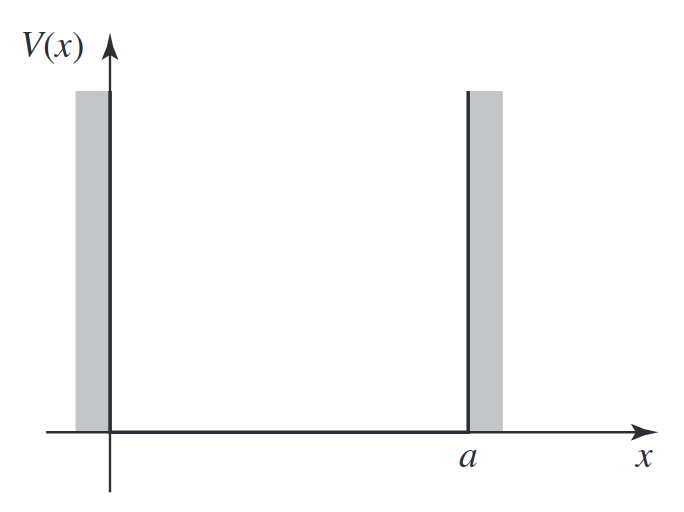
\includegraphics[width=7cm]{images/infinite_square_well.png}
	\caption{Sumur tak hingga}
	\label{img:infinite_square_well}
\end{figure}

Pada aplikasi nya, berdasarkan
\cite{griffithsIntroductionQuantumMechanics2019}, persamaan \ref{eq:tise} dapat
digunakan untuk mencari penyelesaian permasalahan potensial sumur tak hingga,
seperti yang terlihat pada Gambar \ref{img:infinite_square_well}. Solusi dari
potensial sumur tak hingga, diperoleh nilai eigen ($E$) yang dapat dituliskan
sebagai berikut

\begin{equation} \label{eq:eigenvalue_infinite_square_well}
	E_n = \frac{\hbar^2 k_n^2}{2m} = \frac{n^2 \pi^2 \hbar^2}{2ma^2}
\end{equation}

dengan $n = 1, 2, 3, 4, \dots$

\begin{figure}[H]
	\centering
	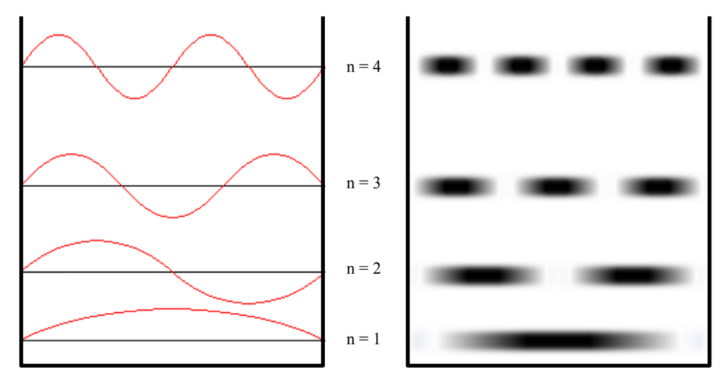
\includegraphics[width=7cm]{images/solution_infinte_square_well.png}
	\caption{Di sebelah kiri adalah fungsi gelombang, di sebelah kanan adalah representasi probabilitas untuk menemukan partikel pada posisi tertentu untuk berbagai keadaan kuantum}
	\label{img:solution_infinite_square_well}
\end{figure}

\noindent
Solusi dari persamaan \ref{eq:eigenvalue_infinite_square_well} merupakan bentuk dari
persamaan sinusoidal. Berdasarkan \cite{dalessandrisSpiralModernPhysics2024},
bentuk grafik nya dapat digambarkan seperti Gambar \ref{img:solution_infinite_square_well}.

% \section{Fisika Komputasi}

% Fisika Komputasi adalah cabang ilmu pengetahuan yang memadukan prinsip-prinsip
% fisika dengan teknik komputasi untuk menyelesaikan masalah yang kompleks dan
% sulit dipecahkan melalui eksperimen atau teori konvensional. Dalam prakteknya,
% Fisika Komputasi memanfaatkan algoritma komputer untuk mensimulasikan sistem
% fisika, dari skala atomik hingga skala astronomis, dan untuk mengolah data
% eksperimental yang besar[1].

% Bidang ini mengemuka seiring dengan kemajuan teknologi komputer, yang
% memungkinkan ilmuwan untuk mengatasi keterbatasan analitis dalam fisika
% tradisional. Dengan menggunakan model dan simulasi komputer, Fisika Komputasi
% mampu memberikan wawasan baru tentang fenomena fisika yang sebelumnya sulit atau
% bahkan tidak mungkin diamati[2].

% Ruang lingkup Fisika Komputasi sangat luas dan mencakup berbagai sub-bidang dalam
% fisika. Beberapa di antaranya adalah:

% \begin{enumerate}
%   \item Mekanika Statistik dan Termodinamika: Penggunaan metode komputasi untuk
%     memahami perilaku sistem dengan banyak partikel, seperti gas, cairan, dan material
%     padat[3].

%   \item Mekanika Kuantum: Simulasi sistem pada skala atomik dan subatomik untuk
%     memahami perilaku partikel seperti elektron dan foton[1].

%   \item Astrofisika: Penggunaan model komputasi untuk mempelajari proses-proses
%     yang terjadi dalam bintang, galaksi, dan alam semesta[2].

%   \item Fisika Material: Pemodelan sifat-sifat material untuk memahami dan
%     merancang material baru dengan karakteristik khusus[2].

%   \item Fisika Partikel: Simulasi interaksi partikel subatomik untuk
%     mengeksplorasi aspek-aspek fundamental dari materi dan energi[1].

%   \item Dinamika Fluida Komputasi (CFD): Penggunaan teknik komputasi untuk
%     mengkaji aliran fluida dan fenomena terkait[3].

%   \item Biofisika dan Sistem Kompleks: Menerapkan metode fisika komputasi untuk
%     memahami sistem biologis dan perilaku kolektif dalam sistem yang kompleks[2].
% \end{enumerate}

% Bidang ini terus berkembang, mengikuti perkembangan teknologi komputasi dan
% algoritma. Peran penting Fisika Komputasi dalam kemampuannya untuk menguji teori,
% mencari parameter yang tidak dapat diakses oleh eksperimen, dan memberikan prediksi
% yang dapat diuji melalui eksperimen atau observasi.

% \subsection{Pengantar Metode Numerik}

% [Isi nya berdasarkan metode numerik yang digunakan]

% Metode numerik dalam Fisika Komputasi adalah teknik-teknik yang digunakan untuk mendekati
% solusi persamaan fisika yang sulit atau tidak mungkin diselesaikan secara analitis.
% Dalam prakteknya, metode numerik memungkinkan ilmuwan untuk mengubah persamaan fisika
% menjadi bentuk yang bisa dihitung dan diselesaikan dengan komputer. Ini menjadi
% sangat penting dalam menghadapi masalah fisika modern yang seringkali terlalu
% rumit untuk diselesaikan dengan metode matematika tradisional[1].

% % Metode Differensial Numerik

% Salah satu aplikasi metode numerik yang paling umum dalam fisika adalah dalam
% penyelesaian persamaan differensial, baik yang bersifat biasa maupun parsial.
% Persamaan ini sering muncul dalam banyak masalah fisika, dari dinamika fluida hingga
% fisika kuantum. Teknik seperti metode Euler, Runge-Kutta, dan metode finite
% difference digunakan untuk mendekati solusi dari persamaan-persamaan ini[2].

% \subsubsection{Metode Monte Carlo}

% Metode Monte Carlo dinamai dari kasino di Monaco, mencerminkan unsur "acak" dalam
% metode ini. Metode ini bergantung pada sampel acak untuk menghasilkan nilai
% numerik. Metode ini sangat berguna dalam kasus di mana solusi analitis sulit diperoleh
% atau bahkan tidak mempunyai solusi analitis, seperti pada perhitungan integral
% berdimensi tinggi atau dalam simulasi sistem yang memiliki banyak variabel
% stokastik \citep{kalosMonteCarloMethods2008}.

% Konsep dasar Metode Monte Carlo dapat diilustrasikan melalui perhitungan integral.
% Misalnya, kita ingin menghitung integral dari sebuah fungsi $f(x)$ dalam interval
% $[a, b]$. Nilai dari integral tersebut dapat didekati sebagai berikut:

% \begin{equation}
%   \int_{a}^{b}f(x) dx \approx \frac{b-a}{N}\sum_{i=1}^{N}f(x_{i})
% \end{equation}

% \noindent
% di mana $x_{i}$ adalah sampel acak dari interval $[a, b]$ dan $N$ adalah jumlah sampel
% yang diambil. Jika $N$ bernilai besar, maka nilai pendekatan nya akan mendekati nilai
% integral nya.

% \begin{figure}[H]
%   \centering
%   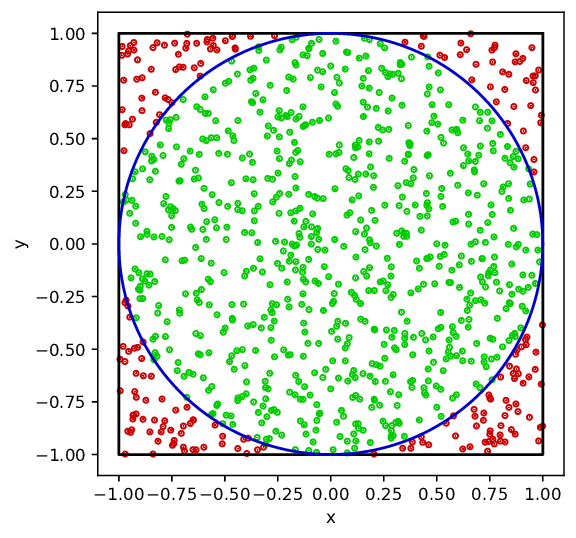
\includegraphics[width=10cm]{
%     images/visualization-of-the-sampled-points-by-the-Monte-Carlo-simulation-to-compute-pi.png
%   }
%   \caption{Contoh simulasi metode monte carlo pada pencarian luas lingkaran}
%   \label{gambar contoh pencarian luasan monte carlo}
% \end{figure}

% Sebagai contoh, metode ini dapat digunakan untuk menghitung area di bawah kurva dari
% seperempat lingkaran. Jika berdasarkan Gambar
% \ref{gambar contoh pencarian luasan monte carlo}, seperempat lingkaran nya kita tarik
% dari $x = 0$ hingga $x = 1$. Secara analitis, seperempat lingkaran tersebut mempunyai
% luasan $L = \frac{1}{4}\pi r^{2}$. Dalam metode monte carlo, nilai nya akan mendekati
% nilai analitis nya dengan cara menjumlahkan titik-titik yang masuk ke dalam seperempat
% lingkaran kemudian membaginya dengan total titik yang ada.

% % Aplikasi dalam Fisika

% Dalam fisika, Metode Monte Carlo digunakan dalam berbagai konteks, seperti dalam
% simulasi dinamika molekuler, fisika partikel, dan fisika statistik. Sebagai contoh,
% dalam dinamika molekuler, metode ini digunakan untuk memprediksi perilaku sistem
% partikel dengan mensimulasikan interaksi mereka selama periode waktu tertentu.

% % Variansi dan Pengurangan Kesalahan

% Salah satu aspek penting dalam Metode Monte Carlo adalah manajemen variansi. Karena
% metode ini bergantung pada sampel acak, hasilnya memiliki variansi yang terkait
% dengan jumlah sampel. Pengurangan kesalahan dapat dicapai dengan meningkatkan jumlah
% sampel atau menggunakan teknik seperti \emph{importance sampling} untuk memilih
% sampel yang lebih representatif \citep{casellaMonteCarloStatistical2004}.

% \subsubsection{Metode Elemen Hingga}

% \emph{Finite Element Method} (FEM) atau dalam bahasa indonesia disebut Metode Elemen
% Hingga (MEH) merupakan metode numerik yang digunakan untuk menyelesaikan permasalahan
% persamaan diferensial parsial. FEM melibatkan proses pemecahan suatu objek atau
% struktur menjadi serangkaian elemen yang lebih kecil. Setiap elemen ini dihubungkan
% melalui titik-titik yang dikenal dengan nama \emph{nodes}. Metode FEM memungkinkan
% penyelesaian masalah yang lebih kompleks dengan mengganti model kontinu dengan model
% diskrit \citep{etsworldsPengertianDanKonsep2018}.

% Berdasarkan \cite{ichrossofilmubarotPerancanganKonstruksiMesin2017}, matematika dasar
% dari FEM melibatkan beberapa langkah berikut:

% \begin{enumerate}
%   \item \textbf{Diskritisasi Struktur}: Struktur dibagi menjadi elemen-elemen hingga,
%     yang dapat berbentuk satu, dua, atau tiga dimensi tergantung kebutuhan.

%   \item \textbf{Pembuatan Persamaan Displacement}: Setiap elemen memiliki persamaan
%     \emph{displacement} yang didasarkan pada bentuknya.

%   \item \textbf{Hubungan \emph{Strain-Displacement} dan \emph{Stress-Strain}}: Hubungan
%     ini penting untuk menghasilkan persamaan pada setiap elemen. Hukum Hooke
%     sering digunakan untuk menghubungkan stress dengan strain.

%   \item \textbf{Matriks Kekakuan}: Persamaan matriks kekakuan dibuat menggunakan
%     metode seperti \emph{direct equilibrium}, \emph{energy method}, atau \emph{weight
%     residual method}.

%   \item \textbf{Persamaan Global dan Boundary Condition}: Persamaan matriks kekakuan
%     dari setiap elemen dikombinasikan untuk membentuk persamaan global. \emph{Boundary
%     condition} diterapkan untuk menyelesaikan permasalahan singular.

%   \item \textbf{Menyelesaikan Degree of Freedom yang Tidak Diketahui}: Ini melibatkan
%     penggunaan metode eliminasi atau iteratif seperti Gauss atau Gauss-Seidel untuk
%     menemukan nilai-nilai yang tidak diketahui.

%   \item \textbf{Analisis Strain dan Stress}: Terakhir, \emph{strain} dan \emph{stress}
%     pada setiap elemen dihitung untuk mendapatkan pemahaman tentang respons
%     struktur terhadap beban yang diterapkan.
% \end{enumerate}

% \section{Julia dalam Fisika Komputasi}

% [Implementasi Julia dalam Fisika Komputasi]

% % \section{Integrasi GPU dalam Fisika Komputasi}

% \section{Penggunaan Julia untuk Komputasi Fisika pada GPU}

% [Mungkin penjelasannya meliputi dasar dasar CUDA.jl dan library serupa]

% =======================================================================

% \section{Persamaan Diferensial Parsial}
% \subsection{Persamaan Diferensial}
% Suatu sistem yang cenderung berubah-ubah terhadap waktu akan lebih mudah untuk digambarkan perubahan yang terjadi ketimbang keadaan mutlak pada saat tertentu. Dalam berbagai bidang keilmuan, persamaan diferensial digunakan untuk menggambarkan perubahan yang terjadi pada suatu sistem. Persamaan diferensial mengandung fungsi yang tidak diketahui (yang merupakan solusi dari persamaan diferensial tersebut) dan beberapa turunannya. Namun, pencarian solusi yang eksplisit seringkali sulit didapat, sehingga dilakukan penyelesaian menggunakan grafik dan pendekatan numerik untuk mendapatkan informasi yang dibutuhkan \citep{stewart_2020_calculus}.  Apabila persamaan tersebut mengandung dua atau lebih variabel bebas, maka persamaan diferensial tersebut merupakan persamaan diferensial parsial (PDP) yang dihitung menggunakan derivatif parsial.
% \subsection{Derivatif Parsial}
% Derivatif parsial dalam sebuah fungsi dengan beberapa variabel adalah derivatif terhadap salah satu variabel, dengan menganggap variabel lainnya konstan \citep{robertalexanderadams_2014_calculus}. Dalam PDP dua variabel $f(x,y)$, misalnya, turunan (derivatif) terhadap $x$ didapat dengan menganggap persamaan tersebut adalah satu variabel dengan menganggap $y$ adalah tetap dan diperlakukan sebagai konstanta \citep{riley_2006_mathematical}. Secara formal, derifatif parsial dari persamaan $f(x,y)$ terhadap $x$ dapat dinyatakan sebagai berikut (dengan menganggap bahwa limitnya ada):
% \begin{equation} \label{partial_limit}
% \frac{\partial f}{\partial x} = \lim_{\Delta x\to\infty} \frac{f(x+\Delta x,y)-f(x,y)}{\Delta x}.
% \end{equation}
% \subsection{Persamaan Diferensial Parsial}
% Berikut akan disajikan sebuah contoh persamaan diferensial parsial:
% \begin{equation} \label{partial_orde_dua}
%     A \frac{\partial^2 u}{\partial x ^2} + B\frac{\partial^2 u}{\partial x \partial y} + C\frac{\partial^2u}{\partial y ^2} = f(x,y),
% \end{equation}
% dengan $x$ dan $y$ merupakan variabel bebas, dan $u$ merupakan solusi yang akan dicari, dan $A, B, C$ merupakan fungsi yang diketahui dari $x$ dan $y$.

% Secara umum, persamaan \eqref{partial_limit} dapat ditulis menjadi persamaan diferensial parsial yang lebih umum menjadi:
% \begin{equation}\label{partial_umum}
%     Lu = f,
% \end{equation}
% dengan $L$ merupakan operator diferensial, $u$ merupakan fungsi yang tidak diketahui (\emph{unknown}) atau solusi yang akan dicari, dan $f$ adalah fungsi yang diketahui. Apabila nilai $f$ pada persamaan \eqref{partial_umum} bernilai  $= 0$, maka persamaan tersebut disebut dengan persamaan diferensial parsial homogen. Sedangkan apabila nilai $f \neq 0$, maka persamaan tersebut disebut dengan persamaan diferensial parsial nonhomogen.

% \subsection{PDP Orde Dua}\label{PDP_orde_dua}
% Pada persamaan diferensial parsial, dikenal istilah orde yang merupakan turunan tertinggi dari fungsi yang ada pada PDP tersebut \citep{riley_2006_mathematical}. Dalam permasalahan fisika, jamak ditemukan pelibatan solusi dari PDP orde dua (yang bentuk umumnya ditampilkan pada Persamaan \eqref{partial_orde_dua})\citep{arfken_2013_mathematical}. Persamaan-persamaan diferensial parsial tersebut menggunakan operator diferensial berupa operator Laplacian: $\nabla ^ 2$. Salah satu contoh dari PDP orde dua yang cukup terkenal dan digunakan adalah persamaan Laplace:
% \begin{equation}\label{laplace_umum}
%     \nabla ^2 u = 0.
% \end{equation}

% Pada persamaan \eqref{laplace_umum} fungsi $u$ dapat berupa potensial gravitasi pada daerah yang tidak mengandung massa, potensial elektrostatis pada daerah tanpa muatan, temperatur keadaan tunak, atau potensial kecepatan untuk fluida mampat tanpa vortisitas dan tanpa sumber atau tenggelam \citep{riley_2006_mathematical}. Intinya, sisi kanan pada persamaan ini menggambarkan keadaan tanpa sumber atau gangguan. Solusi dari persamaan Laplace disebut fungsi harmonik \citep{stewart_2020_calculus}.

% Sejalan dengan persamaan Laplace, persamaan Poisson juga menggambarkan kuantitas fisis yang sama pada persamaan Laplace pada ruas kanannya, hanya saja pada daerah yang mengandung massa, arus listrik, atau sumber panas atau fluida \citep{boas_2006_mathematical}. Persamaan Poisson yang penyelesaiannya akan menjadi bahasan utama di penulisan ini akan dijelaskan pada subbab yang lain.

% Dalam PDP orde dua, persamaan-persamaan yang ada dapat diklasifikasikan menjadi beberapa jenis. Pengklasifikasian ini memberikan panduan mengenai syarat batas dan syarat awal yang tepat dan kehalusan dari solusi analitik. Sama seperti halnya pengklasifikasian irisan kerucut dan bentuk kuadrat ke dalam parabolik, hiperbolik, dan eliptik berdasarkan diskriminan, PDP orde dua juga dapat diklasifikasikan ke kelompok tersebut dengan nilai diskriminan $B^2 - AC$ pada bentuk persamaan \eqref{partial_orde_dua} \citep{yehudapinchover_2013_an}:
% \begin{enumerate}
%     \item $B^2 - 4AC < 0$: Persamaan diferensial parsial eliptik
%     \item $B^2 - 4AC = 0$: Persamaan diferensial parsial parabolik
%     \item $B^2 - 4AC > 0$: Persamaan diferensial parsial hiperbolik
% \end{enumerate}

% Persamaan Laplace dan persamaan Poisson merupakan jenis persamaan diferensial parsial eliptik dengan bentuk:
% \begin{equation}\label{pdp_eliptik}
%     \frac{\partial^2u}{\partial x^2} + \frac{\partial^2u}{\partial y^2}
% \end{equation}
% dengan $A = 1, B = 0, C = 1$, sehingga nilai diskriminannya adalah $0-4(1)(1) = -4 <0$

% \section{Persamaan Poisson}
% Persamaan Poisson adalah sebuah PDP yang menghubungkan antara persamaan Laplace persamaan \eqref{laplace_umum} dengan suku sumber tertentu, seperti yang sudah dibahas pada bagian \ref{PDP_orde_dua}.
% \begin{equation}
%     \nabla^2 u = \rho(\textbf{r})
% \end{equation}
% Fungsi $\rho(\textbf{r})$ inilah yang disebut sebagai suku sumber atau kepadatan sumber. Dalam aplikasi fisiknya, fungsi ini terdiri dari banyak konstanta fisika. Contohnya, jika $u$ adalah potensial elektrostatis pada sebuah ruang, maka $\rho$ adalah kepadatan muatan listrik, sehingga $\nabla^2 u = -\rho(\textbf{r})/\epsilon_{0}$, dengan $\epsilon_0$ adalah permitivitas ruang hampa. Dalam konteks lain, $u$ merupakan potensial gravitasi pada suatu ruang dengan kepadatan materinya diwakili oleh $\rho$; sehingga $\nabla^2 u = 4\pi G \rho (\textbf{r})$ \citep{riley_2006_mathematical}.

% \subsection{Penurunan Persamaan Poisson}
% Bentuk dari Hukum Gauss dapat ditampilkan dalam dua cara: hubungan antara medan listrik $\textbf{E}$ dan muatan listrik total, maupun dalam hubungan antara medan listrik perpindahan $\textbf{D}$ dengan muatan listrik bebas\citep{grant_1990_electromagnetism}. Hubungan antara medan listrik perpindahan $\textbf{D}$ dan muatan bebas digambarkan dengan hubungan sebagai berikut:
% \begin{equation}\label{medan_perpindaha}
%     \nabla \cdot \textbf{D} = \rho_{V}
% \end{equation}
% Seperti diketahui, bahwa $\textbf{D} = \epsilon \textbf{E}$. Sehingga persamaan \eqref{medan_perpindaha} dapat kita tuliskan kembali dengan:
% \begin{equation}\label{epsilon_dot_e}
%     \nabla \cdot (\epsilon \textbf{E}) = {\rho_V}
% \end{equation}
% Dengan asumsi medannya homogen pada ruang hampa, maka $\epsilon$ adalah konsntanta permitivitas ruang hampa:
% \begin{equation}\label{epsilonpindahruas}
%     \nabla \cdot \textbf{E} = \frac{\rho_V}{\epsilon}
% \end{equation}
% Hubungan antara medan listrik $E$ dan potensial listrik $V$ dapat digambarkan dengan persamaan \eqref{medan_listrik}:
% \begin{equation}\label{medan_listrik}
%     \textbf{E} = -\nabla V.
% \end{equation}
% Dalam persamaan tersebut dikatakan bahwa medan listrik merupakan gradien dari potensial skalar \citep{davidjeffreygriffiths_2018_introduction}. Maka persamaan \eqref{epsilonpindahruas} dapat kita tulis ulang menjadi:
% \begin{equation}
%     \nabla \cdot (\nabla V) = - \frac{\rho_V}{\epsilon}
% \end{equation}
% \begin{equation}\label{poisson umum}
%     \nabla ^2 V = - \frac{\rho_V}{\epsilon}
% \end{equation}
% Persamaan \eqref{poisson umum} merupakan persamaan Poisson.

% \section{Metode Numerik}
% \subsection{Motivasi}
% Dalam penyelesaian PDP, secara umum terdapat dua metode: metode analitikal dan metode numerik. Metode analitikal merupakan metode perhitungan langsung untuk mendapatkan perhitungan yang eksak. Namun, seringkali metode analitik tidak dapat menjangkau solusi dari PDP. Sehingga dibutuhkan pendekatan numerikal untuk mencari pendekatan numerik pada solusi PDP.

% Berbagai penyelesaian dengan metode numerik membutuhkan metode iteratif, bahkan kadang rekursif, sehingga dibutuhkan teknologi yang dapat melakukan metode numerik secara cepat. Kini perhitungan metode numerik dapat dilakukan secara komputasional lewat berbagai aplikasi maupun pemrograman. Fokus pada metode ini adalah memodelkan PDP secara numerik sehingga dapar didiskritisasi melalui simulasi komputer \citep{wick_2022_numerical}.

% Mengembangkan dan menganalisa algoritma untuk memecahkan masalah PDP dengan komputer adalah bagian dari metode numerik, yang merupakan bagian dari komputasi saintifik. Komputasi saintifik terbagi menjadi tiga bidang \citep{wick_2022_numerical}:
% \begin{enumerate}
%     \item Pemodelan matematika dan analisis objek
%     \item Pengembangan metode numerik dan algoritma yang efisien dan dapat diandalkan, serta analisanya
%     \item Pengembangan menggunakan perangkat lunak riset (implementasi dari algoritma yang ada)
% \end{enumerate}
% Yang menjadi tugas kunci (\emph{key task}) dari bidang tersebut adalah perancangan dan analisa algoritma. Tujuan utama dari algoritma adalah meformulasi sebuah skema sehingga dapat diimplementasikan ke komputer untuk menjalankan simulasi numerikal. Ada skema yang langsung yang memecahkan masalah hingga ke pembulatan kesalahannya (\emph{error}) seperti halnya eliminasi Gaussian, ada juga skema yang iteratif yang memberikan perkiraan pada solusi sampai pada akurasi tertentu, seperti halnya iterasi Richardson untuk memecahkan sistem persamaan linear. Algoritma dapat dianalisa pada akurasi, efisiensi, dan ketahanannya.

% Dalam perhitungan numerik PDP secara umum, akan ditemukan ralat (\emph{error}) yang merupakan selisih dari hasil pendekatan numerik dengan hasil yang eksak. Misal sebuah PDP diajukan dalam ruang fungsi dan dianalisa:
% \begin{itemize}
%     \item Ruang fungsi $V$ dari solusi eksak $u$ (mungkin tidak diketahui). Maka $u \in V$.
%     \item Ruang fungsi $\Tilde{V}$ dari solusi pendekatan $\Tilde{u}$. Maka $\Tilde{u} \in \Tilde{V}$
% \end{itemize}
% Diskretisasi numerik pada ruang dan waktu menghasilkan parameter $h$ dan $k$ untuk menghitung solusi pendekatan, yaitu $\Tilde{u}:=u_{hk}$. Kemudian dapat digambarkan diskretisasi ralat adalah
% \begin{equation}
%     \left \lvert u - u_{kh} \right \rvert \rightarrow  0 \quad untuk \quad  h \rightarrow 0, k \rightarrow 0
% \end{equation}
% Diskretisasi ralat ini adalah salah satu sumbanngan ralat pada hasil perhitungan PDP dengan metode numerik. Sumbangan ralat lainnya masih sangat mungkin akan terjadi sehingga harus dapat diterima bahwa kita tidak bisa menghindari ralat. Namun yang terpenting adalah mengontrol ralat dan menemukan pembahasan yang tepat apabila ralat yang dihasilkan terlalu besat sehingga memengaruhi interpretasi terhadap simulasi numerik, atau bahkan pembahasan yang tepat saat ralat dapat diabaikan.

% Dalam \cite{richter_2017_einfhrung} (via \cite{wick_2022_numerical}), disimpulkan bahwa ada tujuh aspek yang merupakan karakteristik pemodelan numerik:
% \begin{enumerate}
%     \item Aproksimasi
%     \item Konvergen
%     \item Orde kekonvergenan
%     \item Ralat
%     \item Estimasi ralat
%     \item Efisiensi
%     \item Stabilitas
% \end{enumerate}

% Selanjutnya, akan disebutkan beberapa metode numerik yang lazim digunakan pada penyelesaian PDP:
% \begin{enumerate}
%     \item Metode beda hingga
%     \item Metode garis
%     \item Metode elemen terbatas
%     \item Metode diskretisasi gradien
%     \item Metode volume hingga
%     \item Metode spektral
%     \item Metode tanpa \emph{mesh}
%     \item Metode dekomposisi domain
%     \item Metode \emph{multigrid}
%     \item Metode Gauss-Seidel
% \end{enumerate}
% Metode beda hingga merupakan metode yang paling mudah dan sering digunakan. Metode elemen hingga dan volume hingga sering digunakan pada bidang keteknikan dan komputasi fluida dinamik, dan cocok untuk permasalahan geometri yang rumit. Metode spektral secara umum paling akurat, dan hasilnya cukup halus.

% Pada tulisan ini, akan digunakan metode Gauss-Seidel sebagai penghasil data latih dan data uji, serta sebagai pembanding dari metode \emph{machine learning} yang akan digunakan.

% \section{Metode Gauss-Seidel}
% \subsection{Skema Numerik}
% Sebagai metode iteratif, metode Gauss-Seidel memiliki karakteristik umum untuk mereformulasi bentuk
% \begin{equation}\label{linear}
%    A\textbf{X} = \textbf{B}
% \end{equation}
%  menjadi
% \begin{equation}
%     \textbf{x}^{(n+1)} = M\textbf{x}^{(n)} + \textbf{c}
% \end{equation}
% dengan $n$ merupakan jumlah iterasi dan $M$ merupakan matriks iterasi dan $c$ merupakan vektor baru yang terbentuk dari proses reformulasi \citep{Blackledge2006}.

% Pada persamaan \eqref{linear}, $A$ merupakan matriks persegi nonlinear dengan orde $N$, $X = (x_1, x_2, ..., x_N)^T$ adalah vektor yang tidak diketahui, dan $B$ merupakan matriks yang diketahui. Persamaan \eqref{linear} terdiri dari $N$ persamaan aljabar linear:
% \begin{equation}\label{linear_matriks}
%     \begin{split}
%         a_{11}x_1 + a_{12}x_2 +        ...       + a_{1N}x_N = b_1,\\
%         a_{21}x_1 + a_{22}x_2 +        ...       + a_{2N}x_N = b_2,\\
%         a_{i1}x_1 + a_{i2}x_2 +    a_{ii}x_i     + a_{iN}x_N = b_i,\\
%         a_{N1}x_1 + a_{N2}x_2 +        ...       + a_{NN}x_N = b_N.\\
%     \end{split}
% \end{equation}
% Diasumsikan akan di selesaikan permasalahan \eqref{linear_matriks} secara iteratif. Dimulai dengan menginisialisasi dengan vektor aproksimasi $X^0 = (x_1^0, x_2^0, ..., x_N^0)^T$ yang berikutnya akan dijadikan solusi aproksimasi pada iterasi ke-$r$, $X^r = (x_1^r, x_2^r, ..., x_N^r)^T$. Dari nilai $X^r$ akan dicari aproksimasi yang lebih baik untuk nilai $X^{r+1}$.

% Dalam metode Gauss-Seidel, terdapat pengembangan dari nilai konvergensi dibandingkan metode iteratif serupa, metode Jacobi. Pada metode Gauss-Seidel (atau metode perpindahan berturut), nilai yang ditemukan sebelumnya $x_1^{r+1}, x_2^{r+1}, ..., x_{i-1}^{r+1}$ digunakan untuk menyelesaikan persamaan ke-$i$ untuk $x_i^{r+1}$. Sehingga bentuk umum solusinya menjadi:

% \begin{equation}\label{konfigurasi gauss seidel}
%     \begin{split}
%         x_i^{r+1} = \frac{1}{a_{ii}} \left(b_i-\sum_{j=1}^{i-1}a_{ij}x_j^{r+1} - \sum_{j=i+1}^N a_{ij}x_j^r \right)\\
%         x_N^{r+1} = \frac{1}{a_{NN}} \left(b_N-\sum_{j=1}^{N-1}a_{Nj}x_j^{r+1}\right)
%     \end{split}
% \end{equation}

% \subsection{Formalisme Umum}

% Pada persamaan \eqref{linear}, matriks $A$ dapat dibagi menjadi diagonal bawah $L$, diagonal $D$ dan diagonal atas $U$:

% \begin{equation}
%     A = L + D + U.
% \end{equation}

% Kemudian,

% \begin{equation}
%     \begin{split}
%         (L+D+U)x=b,\\
%         Dx=-Lx-Ux+b,
%     \end{split}
% \end{equation}

% dan

% \begin{equation}
%     x = -D^{-1}Lx - D^{-1} Ux+D^{-1}b
% \end{equation}
% dengan
% \begin{equation}
%     D^{-1} = diagonal(a_{11}^{-1}, a_{22}^{-1},...,a_{nn}^{-1}).
% \end{equation}
% Kemudian metode Gauss-Seidel dapat ditulis sebagai berikut:

% \begin{equation}
%     x^{n+1} = -D^{-1}Lx^{n+1}-D^{-1}Ux^n+D^{-1}b,
% \end{equation}

% dan setelah disusun ulang menjadi

% \begin{equation}
%     x^{n+1} = -(D+L)^{-1}Ux^{n}+(D+L)^{-1}b = Mx^n+c
% \end{equation}

% \subsection{Penambahan Parameter Relaksasi}
% Secara umum, metode Gauss-Seidel dapat dikembangkan dengan menambahkan parameter \emph{sucessiver over-relaxation} (SOR) \citep{Bottoni2022}. Vektor $X^{r+1}$ yang diperoleh dari persamaan \eqref{konfigurasi gauss seidel} dianggap sebagai nilai sementara, misalkan $X^*$, dan nilai yang lebih baik dicari menggunakan persamaan:

% \begin{equation}\label{gauss seidel with provisional value}
%     X^{r+1} = X^r + \omega(X^* - X^r).
% \end{equation}

% yang merupakan bentuk simplikasi dari persamaan:
% \begin{equation}\label{metode relaksasi}
%     x_i^{r+1} = x_i^k+\frac{\omega}{a_{ii}} \left(b_i-\sum_{j=1}^{i-1}a_{ij}x_j^{r+1} - \sum_{j=i+1}^N a_{ij}x_j^r \right)
% \end{equation}

% Persamaan \eqref{gauss seidel with provisional value} menunjukkan bahwa nilai yang lebih baik $X^{r+1}$ dicari dengan menambahkan solusi sebelumnya $X^r$ dengan kenaikan ($X^* - X^r)$ kemudian dikali dengan parameter $\omega$, yang disebut dengan parameter relaksasi. Metode relaksasi menggunakan parameter relaksasi $\omega$ untuk 'menyetel' sistem agar jumlah iterasi yang dibutuhkan berkurang. Untuk alasan stabilitas, $\omega$ harus berada pada rentang ($0 \le \omega \le 2).$ Skema \eqref{gauss seidel with provisional value} disebut \emph{successive under-relaxation} (SUR) apabila $\omega \le 1$ dan \emph{successive over-relaxation} apabila $1 < \omega \le 2$. Saat $\omega$ = 1, $X^{r+1} = X^*$, yang artinya persamaan Gauss-Seidel.

% Konvergensi persamaan Gauss-Seidel dapat diperiksa dengan kriteria toleransi larat yang diinginkan $\varepsilon_s$ \citep{chapra2015}:
% \begin{equation}
%     |\varepsilon_{ij}| = \left|\frac{x_{ij}^n-x_{ij}^{n-1}}{x_{ij}^n}\right| 100\% < \varepsilon_s,
% \end{equation}
% dengan $\varepsilon_{ij}$ merupakan ralat dari sebuah titik pada koordinat yang dihitung dengan mengoperasikan dengan titik yang sama pada iterasi ke-$n$ dan ke-$n-1$.

% \subsection{Metode Gauss-Seidel untuk Penyelesaian Persamaan Poisson di Koordinat Kartesian Dua Dimensi}
% Persamaan Poisson dua dimensi pada koordinat kartesian ($x,y$) diberikan oleh persamaan berikut:
% \begin{equation}\label{poisson_kartesian}
%     \left(\frac{\partial^2}{\partial x^2} + \frac{\partial^2}{\partial y^2}\right) \phi_{ij} = \frac{-\rho_{ij}}{\epsilon_{0}}
% \end{equation}

% Potensial listrik yang akan dicari yang berada pada titik $i$ dan $j$ pada bidang kartesian diwakili oleh simbol $\phi$. Distribusi partikel direpresentasikan oleh $\rho$ dan permitivitas bahan oleh $\epsilon_0$. Pembaruan langkah dari $x$ dan $y$ diwakili oleh simbol $\Delta x$ dan $\Delta y$. Kemudian $\phi(x,y)$ didiskretisasi pada titik ($x_i, y_j$). Titik ($x_i, y_j$) akan ditulis sebagai indeks ($i,j$) dan komponen $\phi(x,y)$ ditulis sebagai $\phi_{i,j}$. Dengan diasumsikan bahwa ada sebanyak $M$ titik sepanjang arah $x$ dan $N$ titik sepanjang arah $y$ yang membentuk \emph{mesh}, maka $i = 1, 2, ..., M$ dan $j = 1,2, ...,N$. Ukuran langkah sepanjang arah $x$ diwakili oleh $\Delta x$ dan arah $y$ oleh $\Delta y$. Untuk $x,y \neq 0$, digunakan skema \emph{central difference} untuk tiap suku pada persamaan \eqref{poisson_kartesian}:

% \begin{equation}\label{diskrit kartesian}
%     \begin{split}
%         \frac{\partial^2}{\partial x^2} \phi=\frac{\phi_{i+1,j}-2 \phi_{ij}+\phi_{i-1, j}}{\Delta x^2}\\
%         \frac{\partial^2}{\partial y^2} \phi = \frac{\phi_{i,j+1}-2 \phi_{ij}+\phi_{i, j-1}}{\Delta y^2}.
%     \end{split}
% \end{equation}.

% Subtitusi persamaan \eqref{diskrit kartesian} ke \eqref{poisson_kartesian} menghasilkan:

% \begin{equation}
%     \frac{\phi_{i+1,j}-2 \phi_{ij}+\phi_{i-1, j}}{\Delta x^2}+\frac{\phi_{i,j+1}-2 \phi_{ij}+\phi_{i, j-1}}{\Delta y^2} = \frac{-\rho_{ij}}{\epsilon_{0}}.
% \end{equation}

% Dengan mempertimbangkan persamaan \eqref{konfigurasi gauss seidel} untuk iterasi, maka dihasilkan konfigurasi sebagai berikut:

% \begin{equation}
%     -2\left(\frac{1}{\Delta x^2} + \frac{1}{\Delta y^2}\right) \phi_{ij}^{n+1} = -\left(\frac{\phi^{n}_{i+1,j}+\phi^{n}_{i-1,j}}{\Delta x^2}-\frac{\phi^{n}_{i,j+1}+\phi^{n}_{i,j-1}}{\Delta y^2}\right),\\
% \end{equation}

% Disusun ulang menjadi:

% \begin{equation}
%     \phi^{n+1}_{ij} \left(\frac{\Delta y^2 + \Delta x^2}{\Delta x^2 \Delta y^2} \right) = \frac{\left(\frac{\phi^{n}_{i+1,\ j}+\phi^{n}_{i-1,\ j}}{\Delta x^2}\right)+\left(\frac{\phi^{n}_{i,\ j+1}+\phi^{n}_{i,\ j-1}}{\Delta y^2}+\frac{\rho_{ij}}{\epsilon_0}\right)}{2}
% \end{equation}

% \begin{equation}\label{GS_cartesian}
%     \phi_{ij}^{n+1}=\frac{\left(\frac{\phi^n_{i+1,\ j}+\phi^n_{i-1,\ j}}{\Delta x^2}\right)+\left(\frac{\phi^n_{i,\ j+1}+\phi^n_{i,\ j-1}}{\Delta y^2}\right)+\frac{\rho_{i,j}}{\epsilon_0}}{2} \cdot \frac{\Delta x^2 \Delta y^2}{\Delta y^2 + \Delta x^2}
% \end{equation}
% Persamaan \eqref{GS_cartesian} merupakan persamaan penyelesaian Persamaan Poisson dua dimensi pada koordinat kartesian.

% \subsection{Metode Gauss-Seidel untuk Penyelesaian Persamaan Poisson di Koordinat Silinder Dua Dimensi}\label{gauss_seidel_silinder}
% Pada penelitian ini akan digunakan koordinat silinder pada sumbu $r$ dan $z$ (simetri aksial). Persamaan Poisson dua dimensi pada koordinat silinder ($r, z$) diberikan oleh persamaan \eqref{Poisson silinder awal} \citep{Shiferaw2013}:
% \begin{equation}\label{Poisson silinder awal}
%     \nabla ^2 \phi = \frac{\partial^2\phi}{\partial r^2} + \frac{1}{r}\frac{\partial \phi}{\partial r}+\frac{\partial^2\phi}{\partial z^2}=\frac{\rho_{ij}}{\epsilon_0}
% \end{equation}

% Potensial listrik yang akan dicari yang berada pada titik $i$ dan $j$ pada koordinat silinder diwakili oleh simbol $\phi$. Distribusi partikel direpresentasikan oleh $\rho$ dan permitivitas bahan oleh $\epsilon_0$. Pembaruan langkah dari $r$ dan $z$ diwakili oleh simbol $\Delta x$ dan $\Delta y$, Kemudian $\phi(r,z)$ didiskretisasi pada titik ($r_i, z_j$). Titik ($r_i, z_j$) akan ditulis dengan indeks ($i,j$) dan $\phi(r,z)$ ditulis sebagai $\phi_{i,j}$. Dengan diasumsikan bahwa ada sebanyak $M$ titik sepanjang arah $r$, dan $N$ titik sepanjang arah $z$ yang membentuk \emph{mesh}, maka $i = 1,2,...,M, j=1,2,...,N$. Ukuran langkah sepanjang arah $r$ diwakili oleh $\Delta r$ dan arah $z$ oleh $\Delta z$. Untuk $r \neq 0$, digunakan skema \emph{central difference} untuk tiap suku pada persamaan \eqref{Poisson silinder awal}:

% \begin{equation}\label{diskretisasi_poisson_silinder}
% \begin{split}
%     \frac{\partial \phi}{\partial r} = \frac{\phi_{i+1,j}-\phi_{i-1,j}}{2\Delta r}\\
%     \frac{\partial^2 \phi}{\partial r^2} = \frac{\phi_{i+1,j}-2\phi_{i,j}+\phi_{i-1,j}}{(\Delta r)^2}\\
%     \frac{\partial^2 \phi}{\partial z^2} = \frac{\phi_{i,j+1}-2\phi_{i,j}+\phi_{i,j-1}}{(\Delta z)^2}
% \end{split}
% \end{equation}

% Dengan subtitusi persamaan \eqref{diskretisasi_poisson_silinder} ke persamaan \eqref{Poisson silinder awal}, didapat persamaan:

% \begin{equation}
%     \frac{\phi_{i+1,j}-2\phi_{i,j}+\phi_{i-1,j}}{(\Delta r)^2} + \frac{\phi_{i+1,j}-\phi_{i-1,j}}{r_i 2 \Delta r} + \frac{\phi_{i,j+1}-2\phi_{ij}+\phi_{i-1,j}}{(\Delta z)^2}=\frac{-\rho_{ij}}{\epsilon_0}.
% \end{equation}

% Kemudian dilakukan perhitungan menghasilkan:
% \begin{equation}
%     \begin{split}
%         \phi_{ij} &= \frac{\frac{\rho_{ij}}{\epsilon_0}+\left(\frac{\phi_{i+1,j}-\phi{1-1,j}}{r_i2\Delta r}\right)(\Delta r)^2 (\Delta z)^2 + \phi_{i-1,j}\left((\Delta z)^2+(\Delta r)^2\right)}{-2\left((\Delta r)^2 + (\Delta z)^2\right)}\\
%         &+\frac{(\Delta z)^2 \phi_{i+1,j} + \phi_{i,j+1}(\Delta r)^2}{-2\left((\Delta r)^2 + (\Delta z)^2\right)}
%     \end{split}
% \end{equation}
% Dengan mempertimbangkan persamaan \eqref{konfigurasi gauss seidel} untuk iterasi, maka dihasilkan konfigurasi persamaan iterasi Gauss-Seidel untuk persamaan Poisson 2 dimensi di koordinat silinder ($r,z$):

% \begin{equation}\label{GS_silinder}
%     \begin{split}
%         \phi^{n+1}_{ij} = \frac{\frac{\rho_{ij}}{\epsilon_0}+\left(\frac{\phi^n_{i+1,j}-\phi^n_{i-1,j}}{r_i 2 \Delta r}\right)(\Delta r)^2(\Delta z)^2 + \phi^n_{i-1,j}((\Delta z)^2 + (\Delta r)^2) + (\Delta z)^2 \phi^n_{i+1,j} + \phi^n_{i,j+1}(\Delta r)^2}{-2((\Delta r)^2 + (\Delta z)^2)}
%     \end{split}
% \end{equation}

% \section{Syarat Batas}

% Dalam bidang persamaan diferensial, permasalahan nilai batas merupakan persamaan diferensial dengan sekumpulan pembatas tambahan yang disebut syarat batas \citep{zwilinger2022}. Solusi dari persamaan diferensial parsial umumnya tidak unik. Agar unik, persamaan diferensial parsial harus menggunakan syarat batas dan syarat awal \citep{waletPartial}. Syarat batas numerik muncul dalam proses implementasi numerik pada syarat batas fisis tertentu pada keadaan fisis sesungguhnya ataupun cuplikan domain (karena keterbatasan sumber daya komputasi)\citep{Brio2010}. Syarat batas menunjukkan perilaku dari sebuah fungsi pada batas area yang didefinisikan.

% Untuk dapat digunakan, permasalahan nilai batas harus didefinisikan secara jelas. Artinya, bahwa dengan memberikan masukan untuk masalah tertentu, terdapat solusi yang unik yang bergantung terus menerus pada masukan tersebut. Masalah nilai batas memiliki kondisi yang ditentukan pada kondisi ekstrim (batas) dari variabel independen pada persamaan.

% \subsection{Syarat Batas Dirichlet}
% Syarat batas Dirichlet merupakan syarat batas yang menemukan nilai dari fungsi tersebut di syarat batas (syarat batas tipe pertama). Dalam persamaan diferensial parsial, syarat batas Dirichlet digambarkan secara matematis dengan contoh berikut:
% \begin{equation*}
%     \nabla^2 u = f(x),
% \end{equation*}
% dengan $\nabla$ merupakan operator laplace dan $f$ merupakan fungsi yang diketahui, maka syarat batas Dirichlet pada domain $\Omega \subset \textbf{R}^n$ memiliki bentuk:
% \begin{equation}
%     u(x) = f(x)\quad \quad \forall x \in \partial \Omega
% \end{equation}

% Dalam konteks persamaan Poisson, syarat batas Dirichlet dan interiornya diilustrasikan dalam Gambar \ref{gambar dirichlet}.

% \begin{figure}[h]
%     \centering
%     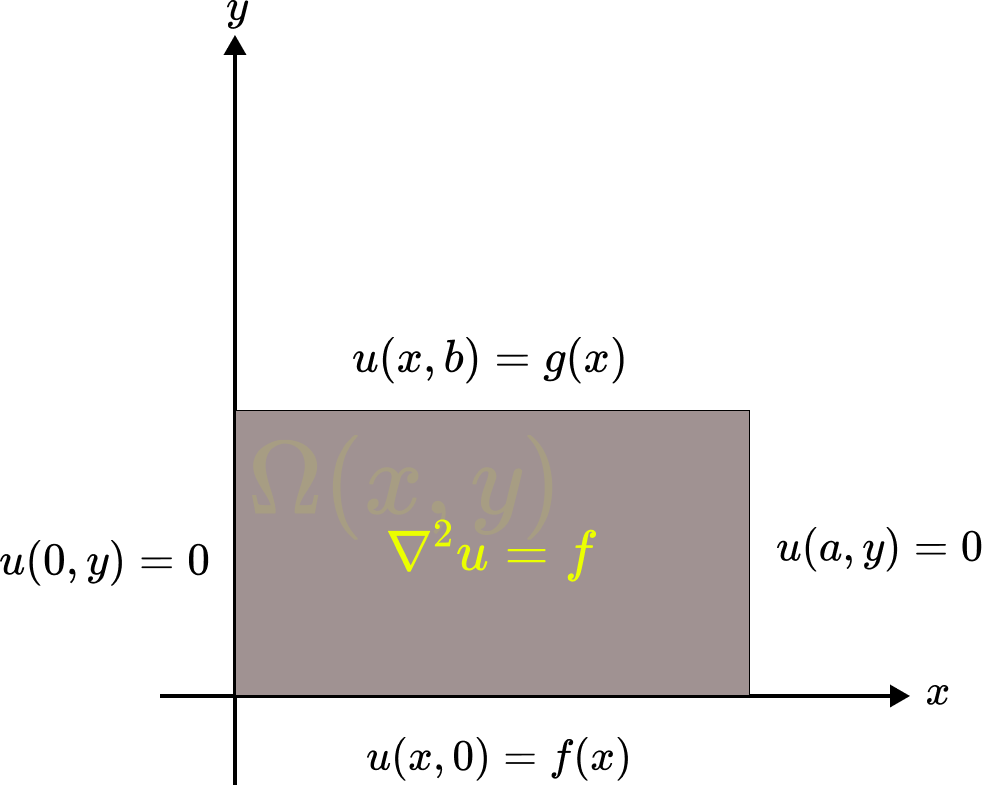
\includegraphics[width=10cm]{gambar/dirichlet.png}
%     \caption{Contoh geometri syarat batas Dirichlet pada persamaan Poisson di koordinat kartesian 2 dimensi ($x,y$) pada domain $\Omega$.\ \emph{Sumber: Penulis}}
%     \label{gambar dirichlet}
% \end{figure}

% \subsection{Syarat Batas Neumann}
% Syarat batas Neumann merupakan syarat batas yang menemukan nilai dari derivatif normal dari fungsi tersebut (syarat batas kedua). Dalam persamaan diferensial parsial, syarat batas Neumann digambarkan secara matematis dengan contoh berikut:
% \begin{equation*}
%     \nabla^2 y + y = f(x),
% \end{equation*}

% dengan $\nabla^2$ melambangkan operator Laplace, maka syarat bentuk syarat batas Neumannya pada domain $\Omega \subset \mathbf{R}^n$ menjadi:
% \begin{equation}\label{NeumannBC}
%     \frac{\partial y}{\partial \textbf{n}}(x) = f(x)\quad \forall x \in \partial \Omega,
% \end{equation}
% dengan $\mathbf{n}$ menunjukkan vektor normal eksterior ataupun interior pada batas $\partial\Omega$, dan $f$ adalah fungsi skalar yang diberikan.

% Derivatif normal yang ditunjukkan pada sisi kiri persamaan \eqref{NeumannBC} didefinisikan sebagai berikut:
% \begin{equation}
%     \frac{\partial y}{\partial\mathbf{n}}(x) = \nabla y (x) \cdot \hat{\mathbf{n}}(x),
% \end{equation}
% dengan $\nabla y (x)$ mewakili gradien dari vektor $y(x)$, $\hat{\mathbf{n}}$ adalah unit normal, dan $\cdot$ sebagai operator \emph{inner product}.

% \section{Pemelajaranan Mesin (\emph{Machine Learning})}
% \subsection{Konsep Umum}
% pemelajaranan mesin (US: \emph{machine learning}) adalah sekumpulan algoritma yang mencoba mengaktifkan kemampuan pemelajaranan komputer, sehingga mereka dapat belajar dari data atau pengalaman masa lalu \citep{bayen_2020_python}.
% Tom Mitchell dapat menggambarkan konsep umum pemelajaranan mesin dengan singkat dan mudah dimengerti pada kata pengantar bukunya: bidang pemelajaranan mesin berkaitan dengan pertanyaan tentang bagaimana membuat program komputer yang secara otomatis meningkat seiring dengan meningkatnya pengalaman \citep{Mitchell1997}.

% Mitchell memberikan sedikit formalisme mengenai pendapatnya tentang konsep umum pemelajaranan mesin tersebut: sebuah program komputer dikatakan belajar dari pengalaman \textbf{E} (\emph{experience}) sehubungan dengan beberapa kelas tugas \textbf{T} (\emph{task}) dan ukuran kinerja \textbf{P} (\emph{performance}), jika kinerjanya pada tugas \textbf{T}, yang diukur dengan \textbf{P}, meningkat dengan pengalaman \textbf{E}.

% Istilah pemelajaran mesin digunakan dalam hal yang sangat umum dan merujuk pada teknik yang umum untuk mengekstrapolasi pola dari kumpulan yang besar atau kemampuan untuk membuat prediksi pada basis data yang baru tentang hal yang dipelajari melalui analisa yang tersedia dari data yang diketahui sebelumnya \citep{zocca_spacagna_slater_roelants_2017}

% \subsection{Tipe-tipe pemelajaranan Mesin}
% Biasanya, pemelajaranan mesin dibagi ke dalam dua kategori: pemelajaranan dengan pengawasan (\emph{supervised learning}) dan pemelajaranan tanpa pengawasan (\emph{unsupervised learning})\citep{zocca_spacagna_slater_roelants_2017}. Pengawasan dalam hal ini adalah pemberian label yang benar atau jawaban dari permasalahan yang akan dipecahkan. Informasi tersebut akan digunakan selama pelatihan (\emph{training}).

% Dalam pemelajaranan dengan pengawasan, berdasarkan pada sifat luarannya, dapat dibagi ke dalam 2 algoritma: klasifikasi (\emph{classification}) dan regresi (\emph{regression}). Klasifikasi adalah algoritma yang mengeluarkan hasil berupa data kategori hasil pemelajaranan mengenai data latih yang diberikan. Sedangkan regresi merupakan algoritma yang menghasilkan data kuantitas dari sebuah data keadaan.

% Dalam pemelajaranan tanpa pengawasan, yang merupakan algoritma tanpa label, dapat dibagi menjadi dua algoritma, yaitu pengklasteran (\emph{clustering}) dan pengurangan dimensi (\emph{dimensionality reduction}). Dalam algoritma pengklasteran, dibutuhkan ciri-ciri tersembunyi dari objek yang digunakan untuk dilakukan pengelompokkan. Algoritma pengurangan dimensi adalah sekelompok algoritma pemelajaranan tanpa pengawasan untuk mengurangi masalah dimensi yang lebih tinggi menjadi dimensi yang lebih rendah \citep{bayen_2020_python}.

% Masih ada banyak tipe-tipe algoritma pemelajaranan mesin yang tidak dibahas karena tidak relevan dengan penelitian ini. Pada penelitian ini sendiri akan menggunakan tipe algoritma \emph{deep learning} untuk regresi, yaitu \emph{convolutional neural network} (CNN).

% \subsection{Analisis Regresi}
% Algoritma regresi merupakan jenis algoritma \emph{supervised learning} yang menggunakan fitur dari data masukan untuk memprediksi sebuah nilai (biasanya nilai kontinyu), seperti harga rumah yang diberi nilai masukan ukuran, usia, jumlah kamar mandi, jumlah lantai, lokasi, dan sebagainya \citep{zocca_spacagna_slater_roelants_2017}. Analisis regresi berusaha untuk mencari nilai dari parameter fungsi yang paling cocok pada dataset masukan. Tujuan utama dari analisis regresi adalah meminimalkan fungsi kerugian dengan mencari parameter yang pantas untuk fungsi pada data masukan yang mendekati data target dengan sangat baik \citep{zocca_spacagna_slater_roelants_2017}.

% Regresi linear pada dasarnya adalah model linear. Misalnya, sebuah model yang mengasumsikan hubungan linear antara variabel masukan ($x$) dan variabel luaran tunggal ($y$). Lebih spesifik, $y$ dapat dihitung dari kombinasi linear dari variabel masukan $x$ \citep{brownlee_2016}.

% Analisis regresi memiliki variabel respon berupa numerik, misalnya seperti memprediksi usia seseorang dari karakteristik orang tersebut. Ada dua langkah dalam membangun model regresi, yaitu:
% \begin{enumerate}
%     \item Langkah pemelajaranan
%     \item Langkah regresi
% \end{enumerate}

% \section{Jaringan Saraf Buatan/ \emph{Neural Network} (NN)}
% \emph{Neural network} merupakan algoritma \emph{deep learning} (pemelajaran dalam) yang merupakan metode yang bersifat hierarkis dan berlapis. Istilah berlapis ini yang kemudian memberi makna pada kata '\emph{deep}'. Disebut demikian karena model ini menggunakan banyak lapisan proses pemrosesan data (\emph{layers}). Setiap lapisan berisi \emph{node} yang melakukan serangkaian kalkulasi matematis dan masing-masing lapisan belajar untuk mengenali fitur yang berbeda dari masukan yang diberikan.

% \emph{Deep learning} khususnya jaringan saraf buatan dapat dipahami sebagai proses pengektrakan otomatis fitur dari data dan menggunakannya untuk melakukan prediksi atau keputusan. Hal ini sangat berbeda dari metode pemelajaran mesin tradisional, yang pendefinisian fitur harus dilakukan secara manual dan kemudian diaplikasikan pada model pemelajaran mesin (Gambar \ref{deepflow})\citep{Li_Li_Gao}

% \begin{figure}[h]
%     \centering
%     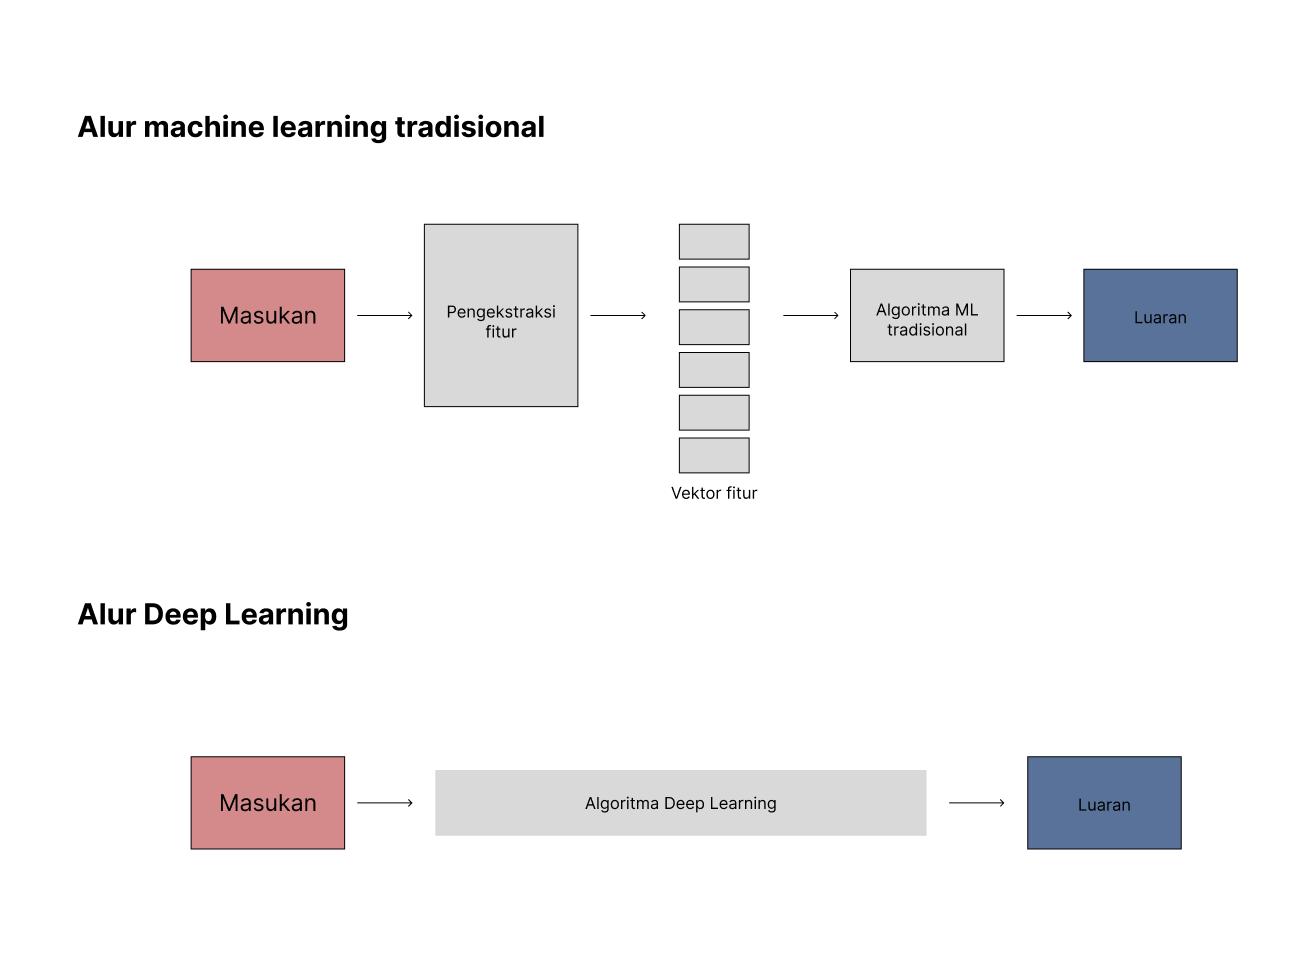
\includegraphics[width=10cm]{gambar/alur_deep_learning.png}
%     \caption{Pemelajaran mesin tradisional membutuhkan ekstraksi fitur secara manual. Pemelajaran dalam (\emph{deep learning}) mengekstrak fitur secara otomatis dengan memberikan input pada lapisannya}
%     \label{deepflow}
% \end{figure}

% Kemudian muncul pertanyaan mengenai awal inspirasi terbentuknya ide dasar mengenai pembentukan jaringan saraf buatan. Seperti halnya banyak penemuan yang diilhami oleh alam, begitupun dalam pembentukan model dari pemelajaran mesin yang cerdas, para ilmuwan berusaha untuk mencari inspirasi ke alam, dan didapatkanlah sebuah pemikiran bahwa algoritma dari sebuah mesin yang cerdas dapat diilhami pula dari sebuah mekanisme yang kompleks dan cerdas, yaitu arsitektur otak manusia \citep{aurélien_géron_2022}. Logika inilah yang menghasilkan jaringan saraf buatan, sebuah model pemelajaran mesin yang diilhami dari jaringan saraf manusia.

% Satuan komputasional paling mendasar pada otak manusia adalah neuron yang saling terkoneksi dengan sinapsis. Setiap neuron menerima sinyal masukan dari dendrit dan menghasilkan sinyal luaran yang ditransmisikan sepanjang akson. Akson tersebut kemudian bercabang dan tersambung melalui sinapsis ke dendrit neuron lain.

% Dalam model komputasional sebuah neuron, sinyal (misalnya $x_0$) yang dihantarkan melalui akson, berinteraksi berkali-kali (misalnya $w_0 x_0$) dengan dendrit lain berdasarkan kekuatan atau bobot sinaptik pada sinapsis yang bersangkutan (misalnya $w_0$). Bobot $w$ ini merupakan parameter yang dapat belajar dan mengontrol kekuatan pengaruh dari suatu neuron ke neuron lainnya.

% Pada model yang sangat standar, dendrit membawa sinyal ke sel tubuh dan semuanya dijumlahkan. Apabila hasil penjumlahan akhir di atas ambang batas, neuron aktif dan meneruskan sinyal melalui akson. Dalam model komputasionalnya, pewaktuan (\emph{timing}) bukanlah hal yang penting, melainkan frekuensi penyampaian informasi. Dari interpretasi ini, kita memodelkan laju aktif dari neuron sebagai fungsi aktifasi $f$ yang merepresentasikan frekuensi lonjakan di sepanjang akson.

% \begin{figure}[ht]
%   \centering
%   \begin{minipage}{0.45\textwidth}
%     \centering
%     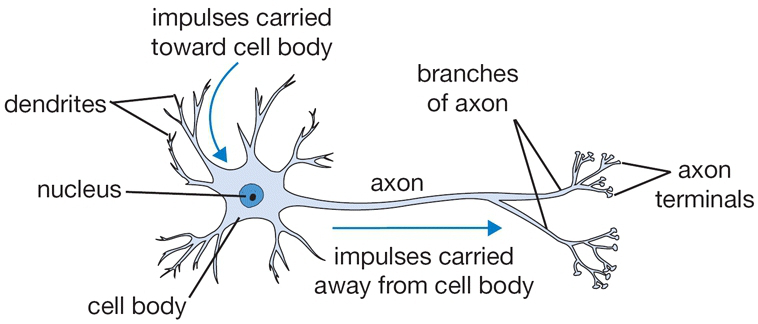
\includegraphics[width=1\linewidth]{gambar/neuron.png} % Adjust the width as necessary
%   \end{minipage}\hfill
%   \begin{minipage}{0.45\textwidth}
%     \centering
%     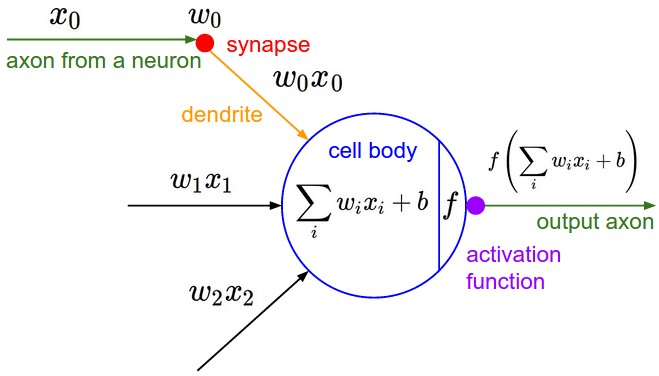
\includegraphics[width=1\linewidth]{gambar/neuron_model.jpeg} % Adjust the width as necessary
%   \end{minipage}
%   \label{neuron_model}
%   \caption{Kiri: Gambaran skema saraf biologis. Kanan: skema model matematis jaringan saraf buatan. \emph{Sumber: CS231n}}
% \end{figure}

% \subsection{Struktur Neural Network}
% Disadur dari \cite{aurélien_géron_2022}, terdiri dari 4 bagian utama:
% \begin{enumerate}
%     \item \emph{Input layer}: Lapisan yang menerima data masukan. Setiap neuron dalam lapisan ini mewakili satu fitur data.
%     \item \emph{Hidden layaer(s)}: Lapisan ini berada di antara lapisan masukan dan luaran. Jumlah lapisan dan neuron dalam bagian ini dapat bervariasi sesuai kompleksitas masalah.
%     \item \emph{Weight connection}: \emph{Weights} atau bobot diterapkan pada tiap sambungan antara node untuk merepresentasikan seberapa penting pengaruh node tersebut pada hasil luaran.
%     \item \emph{Output layer}: Lapisan ini memberikan hasil akhir dari jaringan saraf (selanjutnya, padanan kata \emph{neural network} akan ditulis sebagai jaringan saraf, tanpa kata buatan). Jumlah neuron dalam lapisan ini biasanya sama dengan jumlah kelas dalam masalah klasifikasi atau berjumlah satu neuron dalam masalah regresi.
% \end{enumerate}

% \subsection{\emph{Forward Propagation} (Perambatan Maju)}
% Tahap ini merupakan langkah awal dalam proses belajar sebuah jaringan saraf. Dalam tahap ini, masukan $x$ dikirimkan melalui jaringan dari lapisan masukan ke lapisan luaran. Setiap neuron mengambil $x$ kemudian mengalikan dengan bobot $w$, menambahkan bias $b$ dan kemudian meneruskan hasil melalui fungsi aktivasi \citep{goodfellow_bengio_courville_2016}:
% \begin{equation}
%     s_i = w_i^T x_i +b_i
% \end{equation}

% yang kemudian diikuti oleh fungsi aktivasi nonlinear seperti pada Gambar \ref{feedforward}:
% \begin{equation}
%     y_i = h(s_i)
% \end{equation}

% \begin{figure}[h]
%     \centering
%     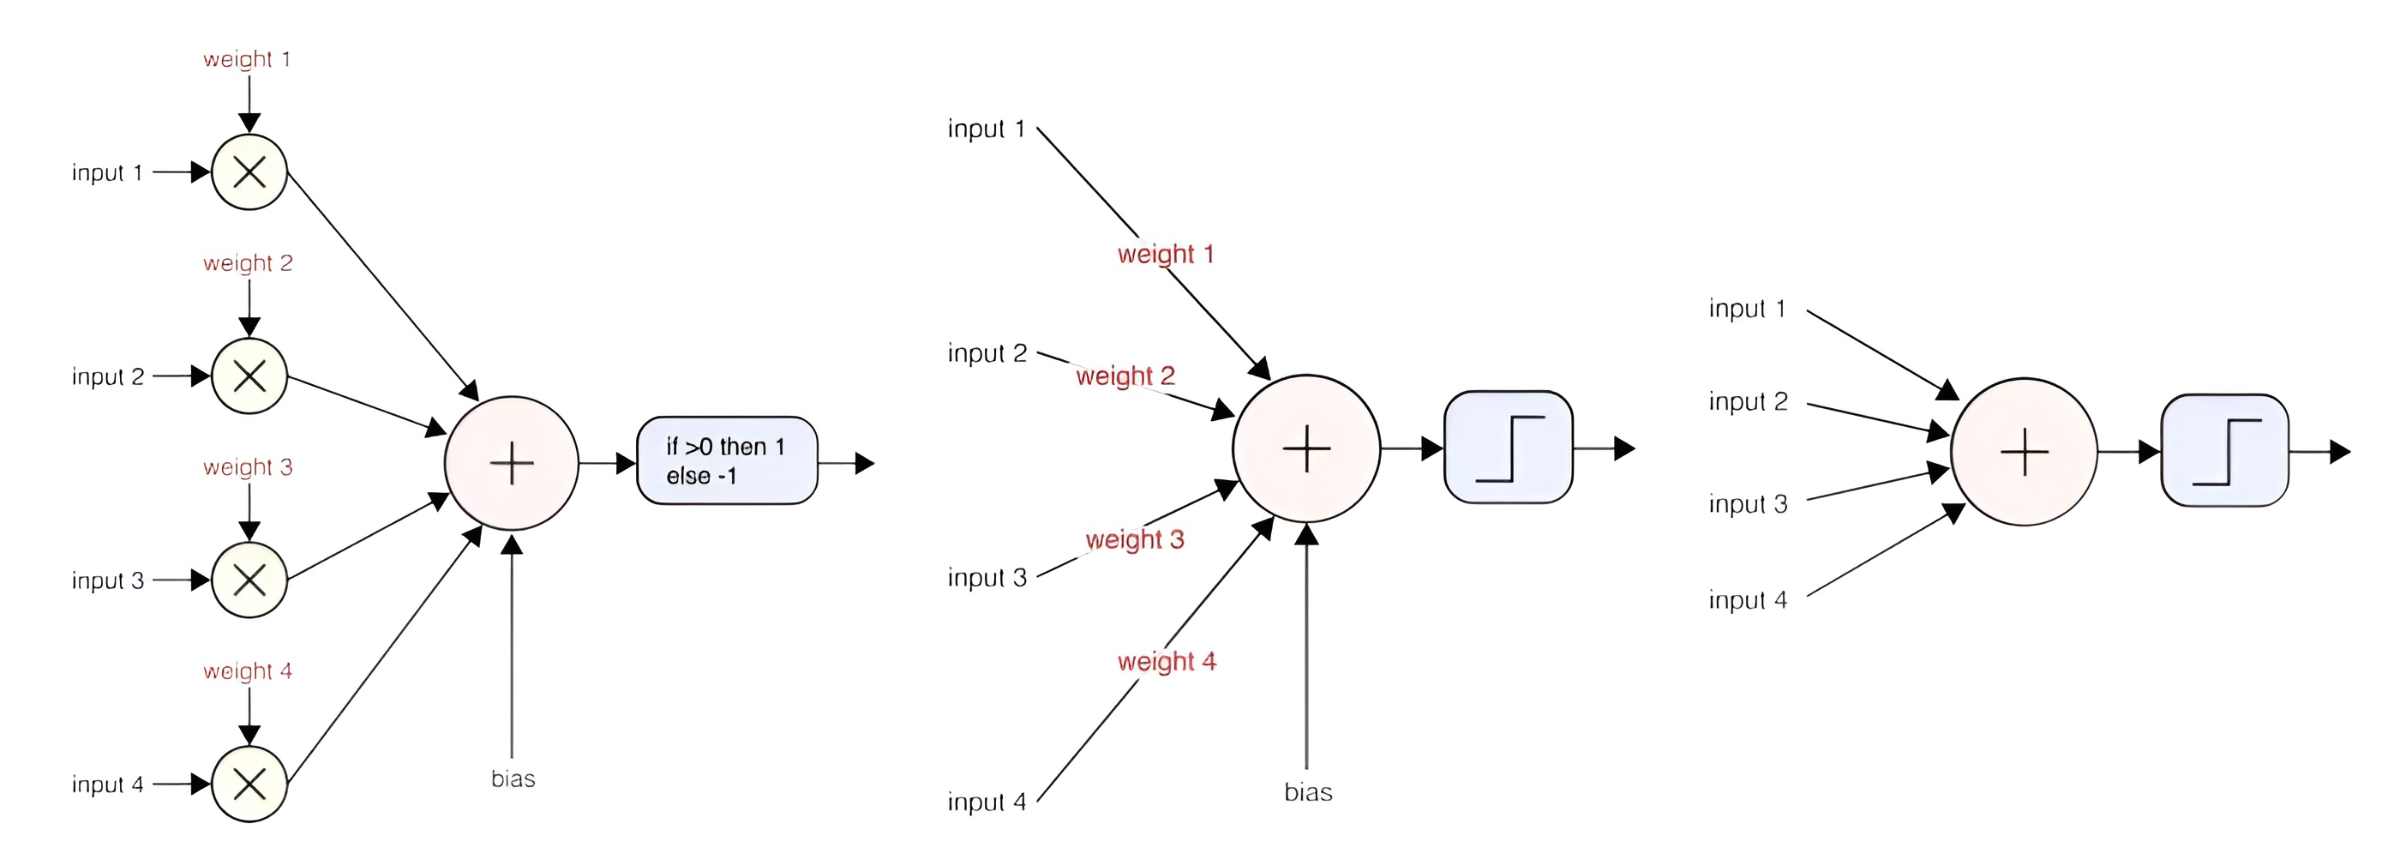
\includegraphics[width=12cm]{gambar/feedforward.png}
%     \caption{Perkalian input dengan bobot pada unit neuron yang kemudian diteruskan dengan operasi dengan fungsi aktivasi. \emph{Sumber: \cite{szeliski_2011}}}
%     \label{feedforward}
% \end{figure}

% $x_i$ merupakan masukan dari unit ke-$i$, $w_i$ dan $b_i$ berturut-turut adalah bobot dan bias yang dapat belajar, $s_i$ adalah luaran dari penjumlahan linear berbobot, dan $y_i$ adalah luaran final setelah $s_i$ masuk pada fungsi aktivasi $h$. Luaran dari tiap tahap lapisan akan menjadi input untuk lapisan selanjutnya. Lapisan pada jaringan saraf terhubung secara berurutan dengan lapisan saraf berikutnya seperti pada Gambar \ref{fully_connected}.

% \begin{figure}[h]
%     \centering
%     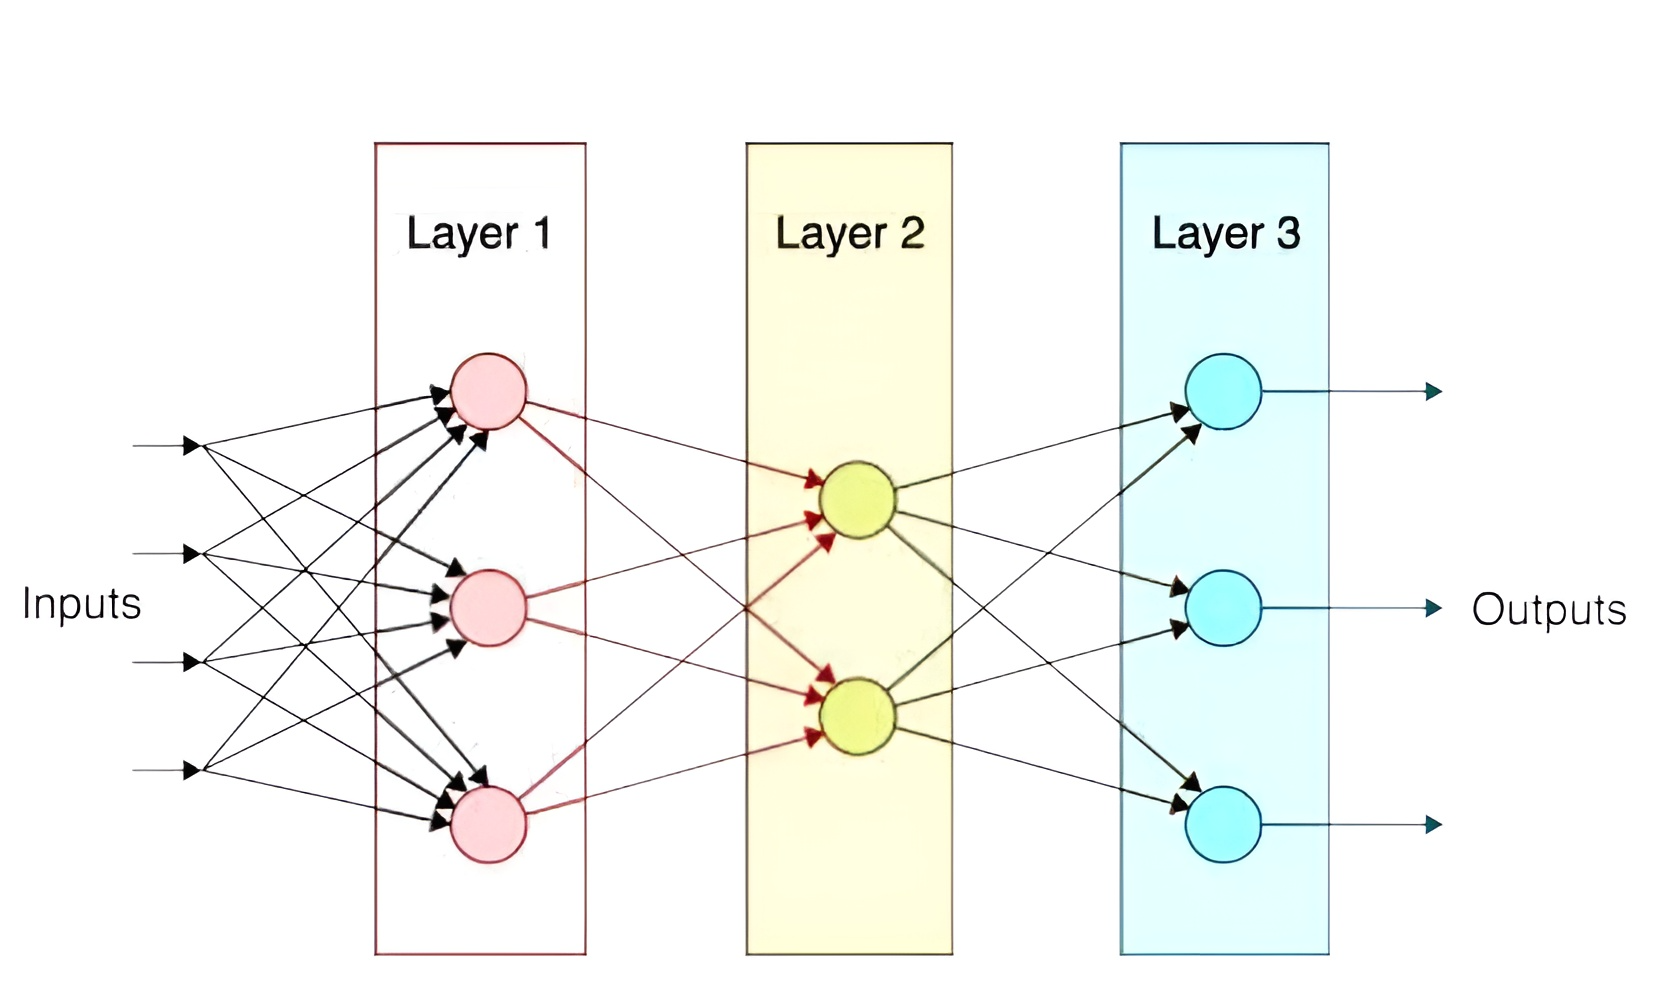
\includegraphics[width=10cm]{gambar/fully_connected.png}
%     \caption{\emph{Fully connected layer} \emph{Sumber: \cite{szeliski_2011}}}
%     \label{fully_connected}
% \end{figure}

% Kita dapat menganggap semua unit dalam lapisan adalah sebuah vektor dengan kombinasi perhitungan linear sebagai berikut:

% \begin{equation}
%     s_l = W_lx_l
% \end{equation}

% dengan $x_l$ adalah masukan pada layer $l$, $W_l$ adalah matriks bobot, dan $s_l$ adalah penjumlahan berbobot. Kemudian kenonlinearan diterapkan berdasarkan elemen untuk dijadikan masukan untuk layer selanjutnya ($l+1$) dengan rumusan:

% \begin{equation}
%     x_{l+1} = y_l = h(s_l)
% \end{equation}

% Lapisan yang menggunakan matriks bobot penuh (padat) untuk kombinasi linier disebut lapisan terhubung penuh (\emph{fully connected layer} (FC)). Jaringan yang hanya berisi FC disebut dengan \emph{multi-layer perceptron} (MLP).

% \subsection{Fungsi Aktivasi}
% Secara biologis, jaringan saraf memiliki neuron yang memiliki fungsi tertentu untuk mengolah impuls tertentu. Begitupun dengan jaringan saraf buatan yang menggunakan fungsi aktivasi, yaitu fungsi yang mendefinisikan keadaan internal neuron untuk menghitung masukkan dari neuron lain \citep{zocca_spacagna_slater_roelants_2017}. Fungsi aktivasi bertugas mengubah masukan neuron menjadi luaran yang akan diteruskan ke neuron selanjutnya. Fungsi aktivasi disebut juga dengan fungsi transfer atau kenonlinearan karena mengubah kombinasi linear dari penjumlahan bobot menjadi model nonlinear dan terletak pada ujung tiap unit atau perceptron untuk memutuskan apakah akan mengaktifkan neuron tersebut \citep{elgendy_2020}. Tujuan dari fungsi aktivasi adalah untuk memperkenalkan nonlinearitas pada jaringan. Tanpa fungsi aktivasi, MLP akan berkelakuan mirip dengan perceptron tunggal, entah berapapun jumlah lapisannya. Fungsi aktivasi dibutuhkan untuk membatasi nilai luaran pada batas tertentu. Ada beberapa fungsi aktivasi, seperti ReLU (Rectified Linear Unit) dan tanh (Gambar \ref{fungsi_aktivasi}).

% Pilihan fungsi aktivasi tergantung pada masalah yang sedang dihadapi dan arsitektur dari jaringan saraf yang digunakan. Pada penelitian ini, akan digunakan dua macam fungsi aktivasi, yaitu ReLU pada \emph{hidden layer} dan tanh pada \emph{output layer}.

% \begin{figure}[ht]
%   \centering
%   \begin{minipage}{0.45\textwidth}
%     \centering
%     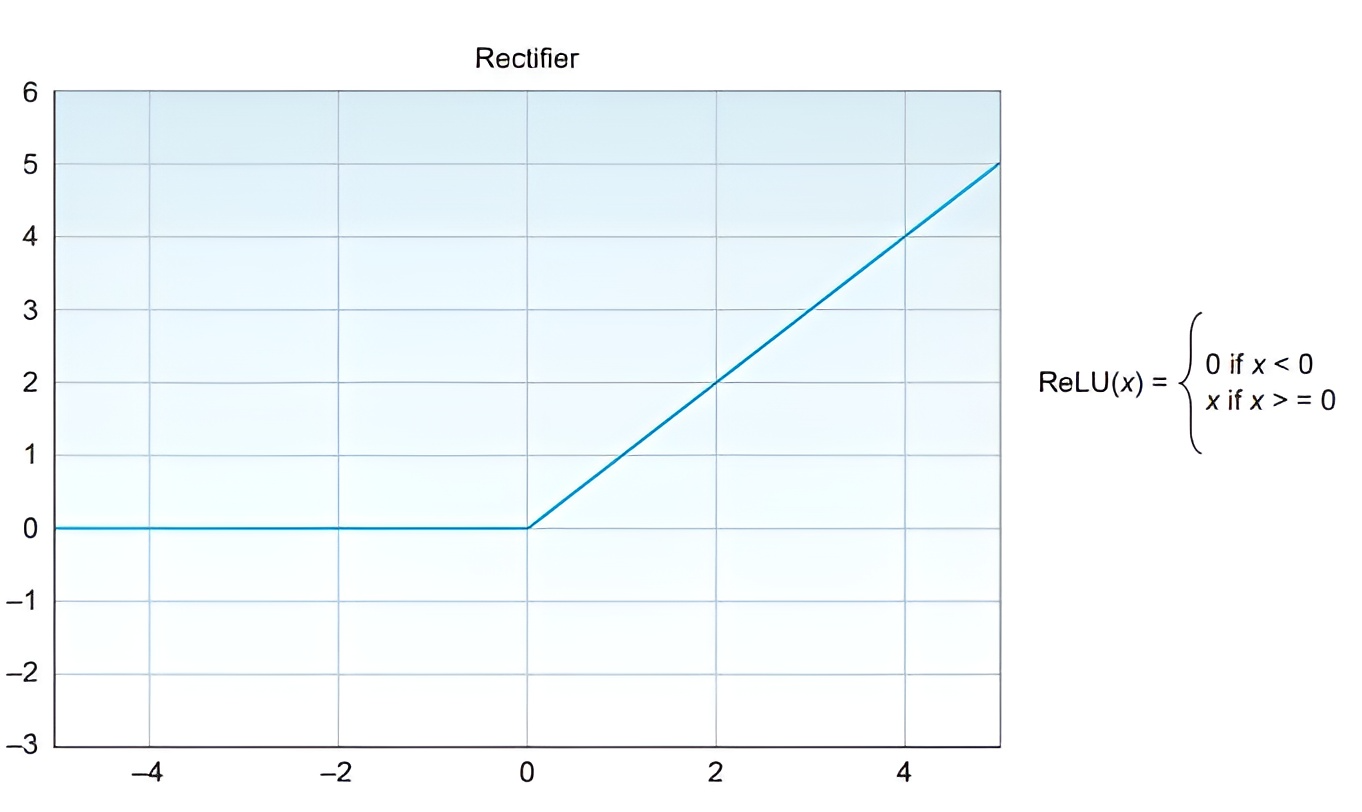
\includegraphics[width=1\linewidth]{gambar/relu1.png} % Adjust the width as necessary
%   \end{minipage}\hfill
%   \begin{minipage}{0.45\textwidth}
%     \centering
%     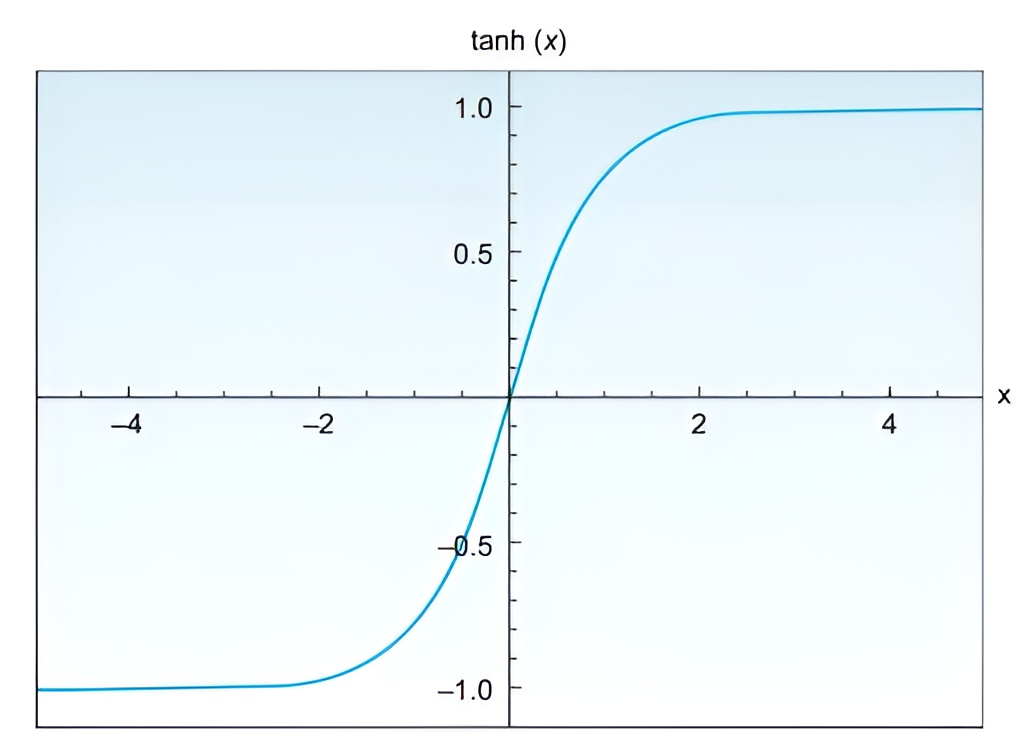
\includegraphics[width=1\linewidth]{gambar/tanh.png} % Adjust the width as necessary
%   \end{minipage}
%   \caption{Kiri: Fungsi aktivasi ReLU mengeliminasi semua nilai negatif dari masukan dengan metransformasi menjadi nilai nol. Kanan: Fungsi aktivasi tanh: apabila nilai masukan sangat besar atau sangat kecil, maka nilai gradien akan sangat kecil; mendekati nol. \emph{Sumber: \citep{elgendy_2020}}}
%   \label{fungsi_aktivasi}
% \end{figure}

% \subsubsection{Fungsi Aktivasi \emph{Rectified Linear Unit} (ReLU)}
% Fungsi aktivasi ReLU adalah fungsi bagian-positif (\emph{positive-part function}) yaitu menghasilkan fungsi identitas untuk argumen (masukkan) positif dan menghasilkan nol untuk masukkan lainnya \citep{Lederer2021}. Fungsi bagian-positif membiarkan masukan positif lewat tanpa diubah, tapi memotong masukan negatif (mengubah masukan negatif menjadi luaran nonnegatif). Secara matematis dapat digambarkan dengan persamaan \eqref{relu} dengan $z$ adalah elemen masukan:
% \begin{equation}\label{relu}
%     ReLU(z) =
%     \begin{dcases}
%         z & \text{jika } z \leq 0 \\
%         0 & \text{jika } z < 0
%     \end{dcases}
% \end{equation}
% Fungsi aktivasi ReLU sering digunakan pada berbagai model jaringan saraf tiruan karena sifat linearitasnya sehingga lebih mudah untuk dilatih dan menghasilkan performa yang lebih baik \citep{elgendy_2020}.

% \subsubsection{Fungsi Aktifasi Tanh (\emph{Hyperbolic Tangent)}}
% Fungsi aktivasi tanh adalah versi pergeseran dari fungsi sigmoid. Singkatnya, pada fungsi sigmoid membatasi nilai luaran pada rentang nilai 0 hingga 1, sedangkan pada tanh, membatasi nilai pada rentang nilai -1 hingga 1. Tanh bekerja dengan lebih baik daripada sigmoid pada karena memliki efek pemusatan data, sehingga memiliki rata-rata data mendekati 0, bukannya 0,5 seperti sigmoid, sehingga membuat pemelajaran untuk lapisan selanjutnya lebih mudah \citep*{elgendy_2020}. Fungsi tanh dirumuskan sebagai berikut untuk nilai masukan $z$:
% \begin{equation}
%     tanh(z) = \frac{sinh(z)}{cosh(z)} = \frac{e^x-e^{-x}}{e^x + e^{-x}}
% \end{equation}

% \subsection{\emph{Backward Propagation} (Perambatan Mundur)}
% Konsep umum yang perlu kita pahami adalah bahwa setiap jaringan saraf adalah pendekatan pada sebuah fungsi. Sehingga hasil yang dihasilkan akan memiliki perbedaan nilai dari fungsi yang didekati. Nilai inilah yang kita sebut dengan kesalahan/ralat (\emph{error}) yang berusaha untuk kita minimalkan nilainya. Karena ralat yang muncul merupakan fungsi bobot (\emph{weights}), maka kita akan mengecilkan ralat terhadap nilai bobot. Secara matematis, himpunan titik-titik yang fungsinya nol mewakili suatu permukaan hiper (\emph{hypersurface}) dan untuk mencari titik minimum pada permukaan ini kita ingin memilih sebuah titik dan kemudian mengikuti kurva ke arah minimum \citep{zocca_spacagna_slater_roelants_2017}. Kesalahan ini kemudian dipropagasi mundur melalui jaringan, yang kemudian bobot antar neuron akan disesuaikan berdasarkan kesalahan tersebut. Proses ini dilakukan berulang-ulang hingga kesalahan mencapai nilai minimum atau setelah jumlah iterasi tertentu \citep{szeliski_2011}. Isitilah yang lebih matematis untuk mendefinisikan tentang perambatan mundur adalah menghitung gradien dari sebuah ekspresi melalui penerapan rekursif dari aturan rantai \citep{Li_Li_Gao}; menghitung gradien dari fungsi $f(\textbf{x})$ di $\textbf{x}$ ($\nabla f(\textbf{x})$) dengan $\textbf{x}$ adalah vektor masukan.

% \begin{figure}[h]
%     \centering
%     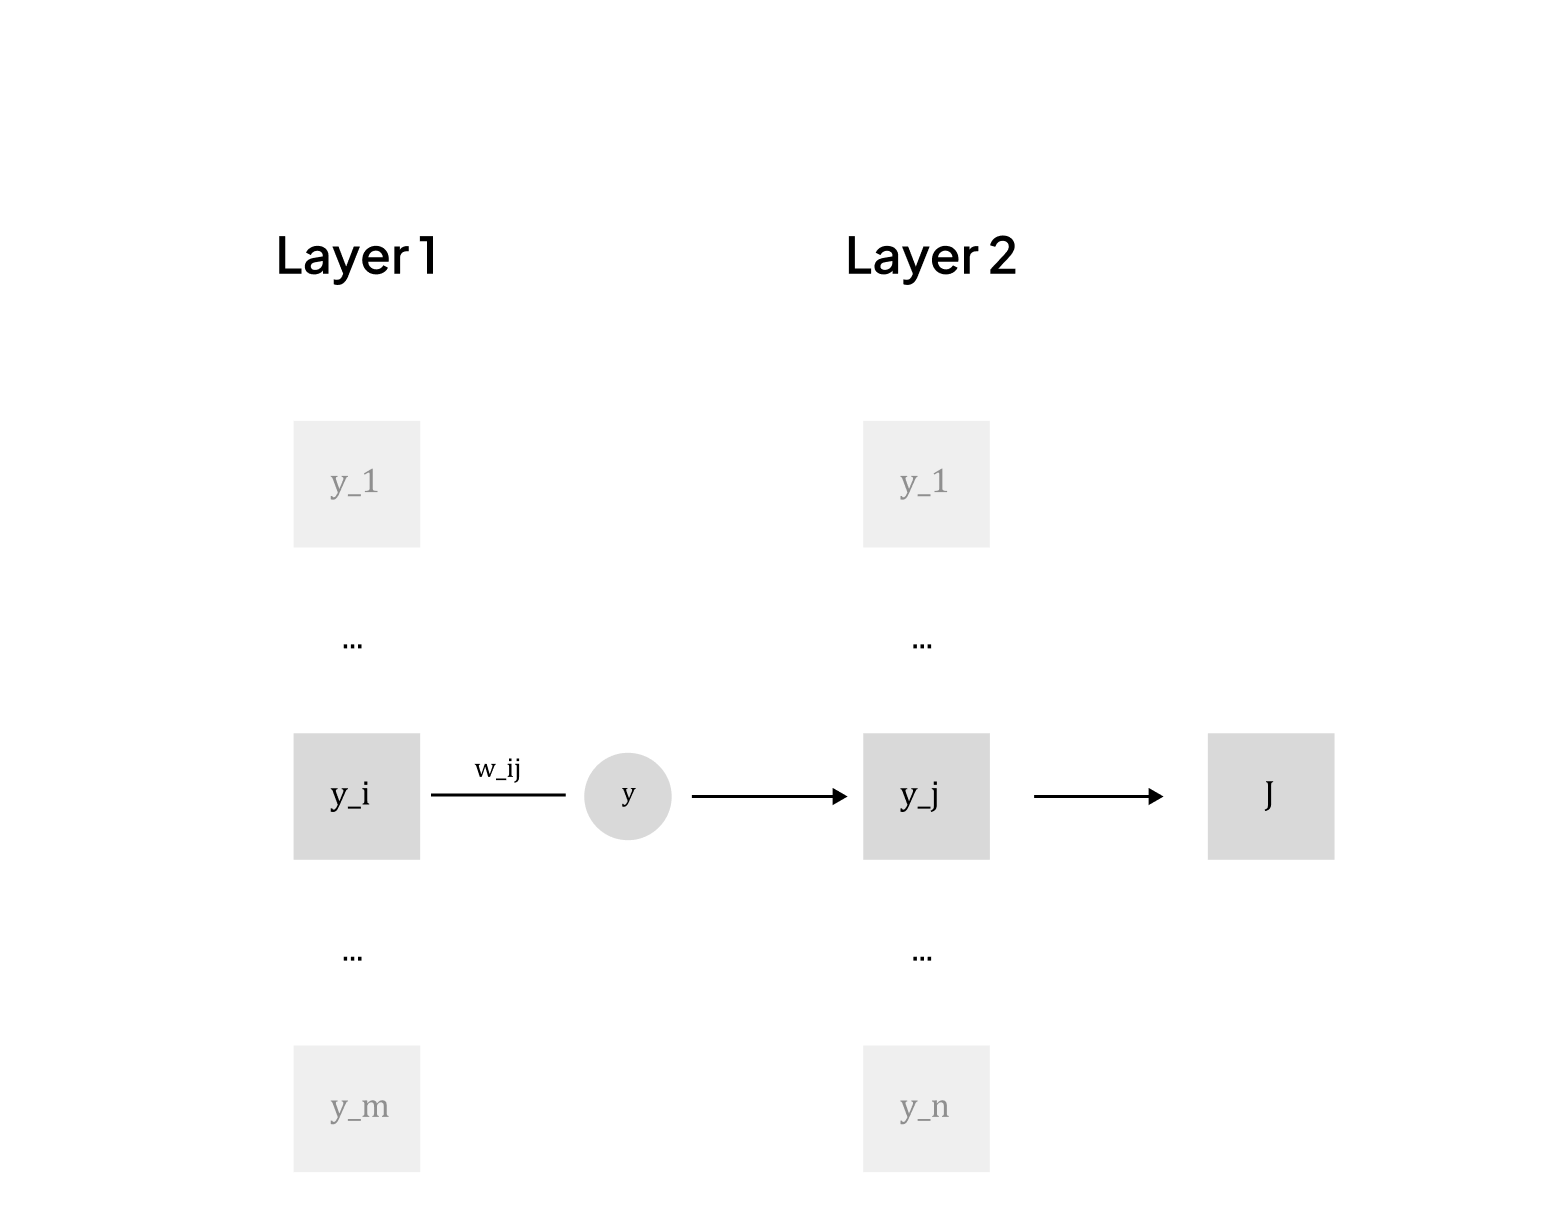
\includegraphics[width=10cm]{gambar/backprop2.png}
%     \caption{Perambatan maju (\emph{forward propagation}. \emph{Sumber: penulis}}
%     \label{backprop}
% \end{figure}

% Sebagai contoh, akan digunakan 2 lapisan, satu sebagai lapisan masukan (\emph{input layer}) dan lapisan lainnya sebagai lapisan luaran (\emph{output layer}) pada Gambar \ref{backprop}. Misal kita notasikan $J$ sebagai galat (error) antara nilai $Layer 2$ dan $Layer 1$, dengan $y$ adalah fungsi aktivasi dengan input dari niai bobot $w_{i,j}$ dan nilai masukan dari \emph{Layer 1} $y_i$ dan luaran adalah nilai $y_j$.

% Tujuan dari perambatan mundur adalah mencari nilai bobot dari nilai galat yang dihasilkan $\frac{\partial J}{\partial w_{i,j}}$. Dengan menggunakan aturan rantai, didapat rumusan:
% \begin{equation}
%     \frac{\partial J}{\partial w_{i,j}} = \frac{\partial J}{\partial y_j} \frac{\partial y_j}{\partial y_i} \frac{\partial y_i}{\partial w_{i,j}}
% \end{equation}

% \subsection{Fungsi Kerugian (\emph{Loss Function})}
% Jaringan saraf dilatih menggunakan \emph{stochastic gradient descent} dan bobot diperbarui menggunakan algoritma perambatan mundur ralat \citep{brownlee_2019}. Dalam rangka mengoptimasi bobot, harus didefinisikan fungsi kerugian (\emph{loss function}) yang diminimalkan selama proses pelatihan \citep{szeliski_2011}.

% Fungsi kerugian mengkuantifikasi jarak antara nilai sesungguhnya dan nilai hasil prediksi dari data target. Kerugian (\emph{loss}) biasanya merupakan angka nonnegatif yang semakin kecil, berarti nilainya semakin bagus \citep{goodfellow_bengio_courville_2016}.

% Dalam optimisasi matematis dan teori keputusan, fungsi kerugian adalah fungsi yang memetakan kejadian atau nilai dari satu atau lebih variabel terhadap nilai kebenaran yang secara intuitif merepresentasikan harga yang terasosiasi dengan kejadian tersebut. Secara sederhana, fungsi kerugian adalah metode untuk mengevaluasi seberapa baik algoritma memodelkan set data \citep{shankar_2022}.

% \subsubsection{Rerata Ralat Kuadrat (\emph{Mean Squared Error}/ MSE)/ \emph{L2 Loss}}\label{mse}
% Untuk permasalahan regresi, fungsi kerugian yang paling umum digunakan adalah MSE atau fungsi kerugian L2 \citep{szeliski_2011}:

% \begin{equation}
%    MSE = \frac{1}{n} \sum\limits_n E_n(\textbf{w}) = \frac{1}{n}\sum\limits_n ||\textbf{y}_n - \textbf{t}_n||^2
% \end{equation}

% dengan $\textbf{y}_n$ merupakan prediksi dari jaringan untuk sampel sejumlah $n$ dan $\textbf{t}_n$ merupakan nilai target dari data latih.

% \subsubsection{Rerata Presentasi Ralat Absolut (\emph{Mean Average Percentage Error}/ MAPE) }
% Contoh lain untuk mengukur kualitas regresi adalah dengan MAPE. MAPE seringkali digunakan karena sangat intuitif diinterpretasikan sebagai ralat relatif \citep{DEMYTTENAERE201638}. Untuk $x$ sebagai masukan dari model regresi, $g$ merupakan model regresi, dan $y$ adalah nilai target dari data latih, maka MAPE dirumuskan dengan:
% \begin{equation}\label{mape}
%     MAPE = \frac{1}{n} \sum \limits_n \left(\frac{|g(\textbf{x})-\textbf{y}|}{|\textbf{y}|}\right)
% \end{equation}

% \section{Jaringan Saraf Konvolusional/ \emph{Convolutional Neural Network} (CNN)}
% \subsection{CNN pada \emph{Deep Learning}}
% \emph{Convolutional Neural Network} (selanjutnya akan disebut dengan CNN) merupakan pengembangan dari jaringan saraf buatan (\emph{artificial neural network (ANN)/ neural network (NN)}). Pada dasarnya, CNN masih sama dengan jaringan saraf reguler. Perbedaan utamanya adalah bahwa arsitektur CNN membuat asumsi secara gamblang bahwa masukannya adalah gambar. Hal ini membuat perambatan maju lebih efisien serta mengurangi jumlah parameter pada jaringan secara signifikan \citep{Li_Li_Gao}.

% Lebih lanjut lagi, meskipun jaringan saraf reguler dapat memecahkan masalah dengan gambar, namun tidak dapat menskala-ulang (\emph{rescale}) keseluruhan gambar. Hal ini menimbulkan masalah karena gambar yang dijadikan masukan tetap pada ukuran asli, sehingga membutuhkan banyak parameter, dan terlalu banyak parameter dapat menyebabkan \emph{overfitting} \citep{Li_Li_Gao}.

% Ide utama dari CNN adalah menggunakan lapisan (\emph{layer}) (biasa disebut dengan filter) yang mempunyai tugas spesifik masing-masing untuk memanipulasi gambar untuk mendapatkan fitur tertentu pada gambar \citep{zocca_spacagna_slater_roelants_2017}. Filter yang telah berisi berbagai macam fitur tersebut akan diteruskan kepada node-node pada \emph{layer} yang lainnya untuk digabungkan dan dikenali berdasarkan hasil latihan yang dilakukan.

% Dalam jaringan saraf reguler, gambar diperlakukan sebagai vektor kolom dengan cara me-\emph{flatten} tanpa memperhatikan hubungan spasial antar piksel \citep{zhang2023dive}. Idealnya, jaringan dapat memanfaatkan pengetahuan bahwa piksel yang berdekatan biasanya terkait satu sama lain, untuk membangun model yang efisien untuk belajar dari data gambar \citep*{zhang2023dive}

% Dari keuntungan mengenai wawasan spasial dari jaringan, dibanding NN, CNN dapat memebentuk model yang lebih akurat dengan cara yang efisien. Hal tersebut dikarenakan CNN membutuhkan parameter yang lebih sedikit dan pada CNN juga lebih mudah untuk diterapkan perhitungan paralel menggunakan \emph{graphic processing unit} (GPU) \citep{chetlur2014cudnn}.

% \subsection{Lapisan Konvolusi (\emph{convolution layer})}
% Setelah kita hijrah dari jaringan saraf reguler ke jaringan saraf konvolusi, kita dikenalkan dengan berbagai keuntungan yang sekaligus menjadi prinsip dalam jaringan saraf konvolusi. Salah satu prinsip tersebut adalah translasi invarian \citep{1992SPIE.1709..257Z}. Hal ini berarti pergeseran pada masukan $\textbf{X}$ membuat pergeseran pada lapisan tersembunyi (\emph{hidden layer}) $\textbf{H}$ (keduanya merupakan matriks 2 dimensi dengan ukuran yang sama). Agar setiap unit/neuron pada lapisan tersembunyi menerima masukan dari tiap unit masukan, penggunaan bobot seperti pada jaringan saraf reguler akan diubha menjadi penggunaan parameter $\textbf{V}$.Dengan $u$ adalah bias (konstan), maka lapisan tersembunyi pada CNN didefinisikan sebagai:

% \begin{equation}\label{konvolusi_real}
%     [\textbf{H}]_{i,j} = u + \sum\limits_a \sum\limits_b [\textbf{V}]_{a,b} [\textbf{X}]_{i+a,j+b}
% \end{equation}

% Persamaan \eqref{konvolusi_real} merupakan persamaan konvolusi. Pada persmaan tersebut, masukan $\textbf{X}$ pada indeks $(i+a, j+b)$ diberikan bobot secara efektif dengan koefisien $[\textbf{V}]_{a,b}$ untuk mendapatkan nilai $[\textbf{H}]_{i,j}$ \citep{zhang2023dive}. Dalam komunitas penelitian pemelajaran mendalam (\emph{deep learning}), \textbf{$V$} dikenal sebagai lapisan konvolusi (\emph{convolution layer}), filter, atau lapisan bobot yang merupakan parameter yang dapat belajar \citep{zhang2023dive}.

% Berdasarkan deskripsi tersebut, pada tiap lapisan, matriks masukan dan matriks konvolusi (\emph{kernel}) memproduksi matriks luaran melalui operasi korelasi silang (\emph{cross-correlation}).

% Operasi korelasi silang ditemukan pada filter atau \emph{kernel} konvolusional yang beroperasi pada  gambar dan melakukan perhitungan \emph{dot product}. Setiap filter akan mengekstrak fitur-fitur yang berbeda dari gambar \citep{patel_2020}.

% Sebagai contoh, akan digunakan \emph{kernel} dengan ukuran $3\times 3$ dan ukuran gambar masukan $5\times 5$. Akan dilakukan perkalian berdasarkan elemen (\emph{element-wise}) antara nilai warna piksel dari gambar yang cocok dengan ukuran filter dengan filter itu sendiri, dan kemudian dijumlahkan untuk mendapatkan nilai tunggal.

% \begin{figure}[h]
%     \centering
%     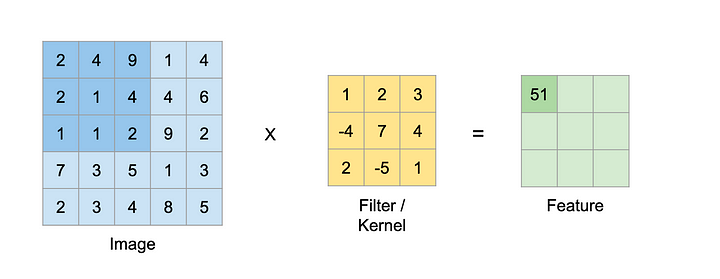
\includegraphics[width=10cm]{gambar/convolution-operation1.png}
%     \caption{Operasi konvolusi pertama. \emph{Sumber: \citep{patel_2020}}}
%     \label{convolution_operation}
% \end{figure}

% Pada Gambar \ref{convolution_operation}, operasi yang dilakukan adalah sebagai berikut:
% $(2 \times 1) + (4 \times 2) + (9 \times 3) + (2 \times (-4)) + (1 \times 7) + (4 \times 4) + (1 \times 2) + (1 \times (-5)) + (2 \times 1) = 51  $

% Kemudian filter konvolusional melanjutkan operasinya dengan bergeser satu sel ke kanan:
% \begin{figure}[h]
%     \centering
%     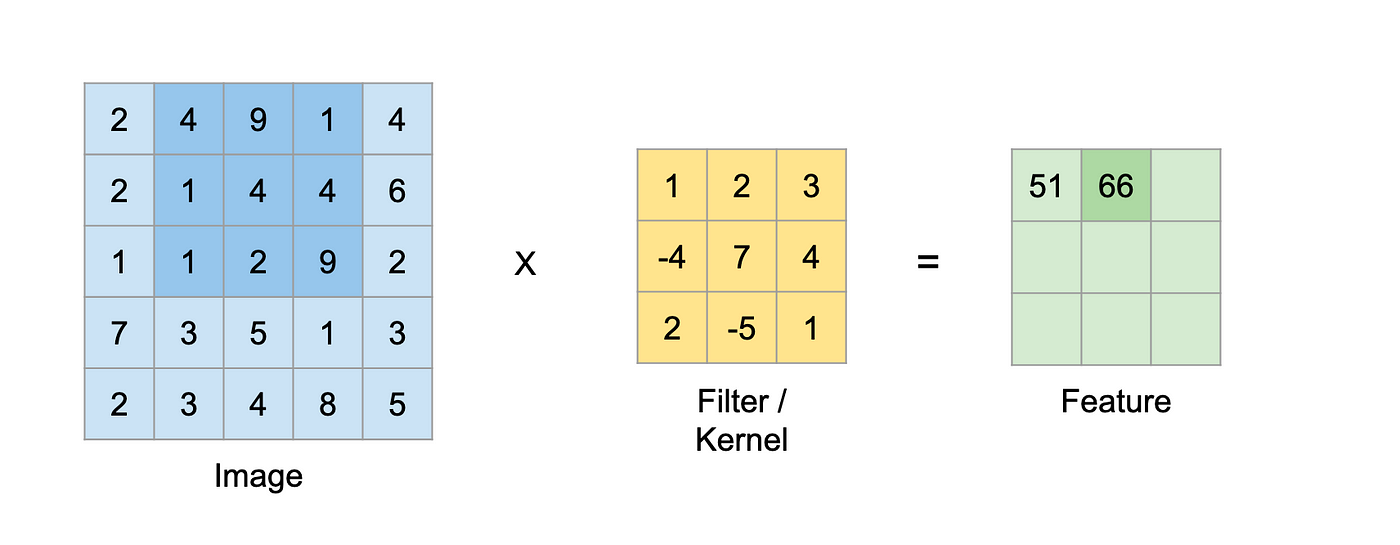
\includegraphics[width=10cm]{gambar/convolution-operation.png}
%     \caption{Operasi konvolusi kedua. \emph{Sumber: \citep{patel_2020}}}
%     \label{operasi_konvolusi_kedua}
% \end{figure}

% Operasi konvolusi dari filter tersebut adalah: $(4 \times 1) + (9 \times 2) + (1 \times 3) + (1 \times (-4)) + (4 \times 7) + (4 \times 4) + (1 \times 2) + (2 \times (-5)) + (9 \times 1) = 66 $

% Filter tersebut akan terus berjalan dari kiri ke kanan, menuju bawah, hingga tiba pada bagian pojok kanan bawah dengan bergeser 1 piksel. Jumlah pergeseran filter ini dinamakan \emph{stride}. Ukuran \emph{stride} berpengaruh terhadap ukuran fitur (\emph{feature}) yang dihasilkan. Sehingga ukuran fitur secara lengkap yang dihasilkan adalah:

% \begin{equation}\label{ukuran_fitur}
%     ukuran\ fitur = \left(\frac{ukuran\ gambar - ukuran\ filter}{\emph{stride}}\right) + 1
% \end{equation}

% Neuron pada lapisan konvolusi pertama tidak terkoneksi pada tiap piksel pada gambar masukan, melainkan hanya piksel pada bidang reseptif (\emph{receptive fields}) (Gambar \ref{receptive_fields}). Selanjutnya, tiap neuron pada lapisan konvolusi kedua hanya terhubung pada neuron yang terletak di dalam persegi kecil pada lapisan pertama. Struktur arsitektur demikian membuat jaringan tersebut berkonsentrasi pada fitur kecil tingkat rendah pada lapisan konvolusi pertama, dan kemudian menyusun fitur-fitur tersebut pada tingkat yang lebih besar di lapisan selanjutnya, dan seterusnya \citep{aurélien_géron_2022}.

% \begin{figure}[h]
%     \centering
%     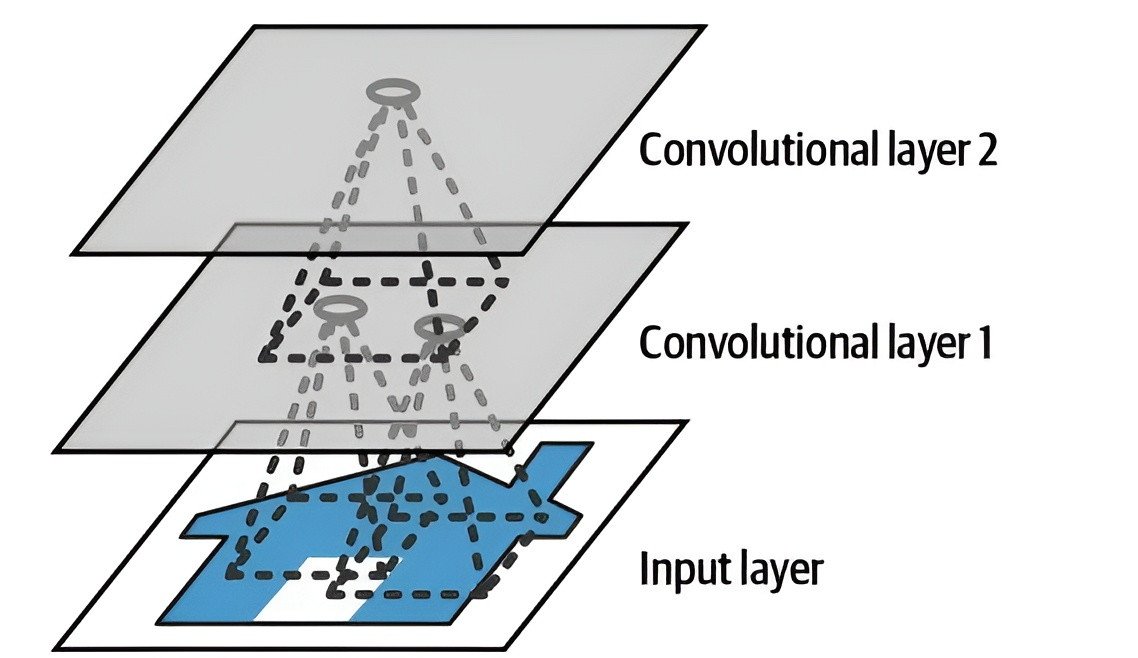
\includegraphics[width=10cm]{gambar/snapedit_1694621260840.png}
%     \caption{Lapisan konvolusi dengan bidang reseptif persegi . \emph{Sumber: \citep{aurélien_géron_2022}}}
%     \label{receptive_fields}
% \end{figure}

% \subsection{\emph{Padding}}
% Dalam persamaan \eqref{ukuran_fitur}, apabila kita aplikasikan pada $240 \times 240$ piksel gambar dengan $10$ layer matriks konvolusi $5 \times 5$, maka akan dihasilkan luaran matriks $200 \times 200$, yang artinya, layer konvolusi mereduksi $30\%$ informasi tentang batas-batas gambar aslinya. Isu demikian dapat diatasi dengan \emph{Padding} \citep{zhang2020dive}.

% \emph{Padding} adalah proses penambahan piksel pada pinggiran gambar asli agar hasil luaran yang diinginkan menjadi lebih besar. Ide awal dari \emph{padding} adalah bahwa piksel di sudut gambar sangat jarang terkena operasi konvolusi sehingga piksel tersebut kurang berkontribusi pada luaran dari operasi konvolusi. Maka ditambahkanlah \emph{padding} pada tepi batas dari matriks masukan agar peran dari piksel tepi digantikan oleh piksel \emph{padding} sehingga luaran yang dihasilkan dapat sama dari masukan. Biasanya digunakan nilai $0$ pada piksel \emph{padding} (disebut dengan istilah (\emph{zero-padding}) \citep{Li_Li_Gao}.

% \begin{figure}[h]
%     \centering
%     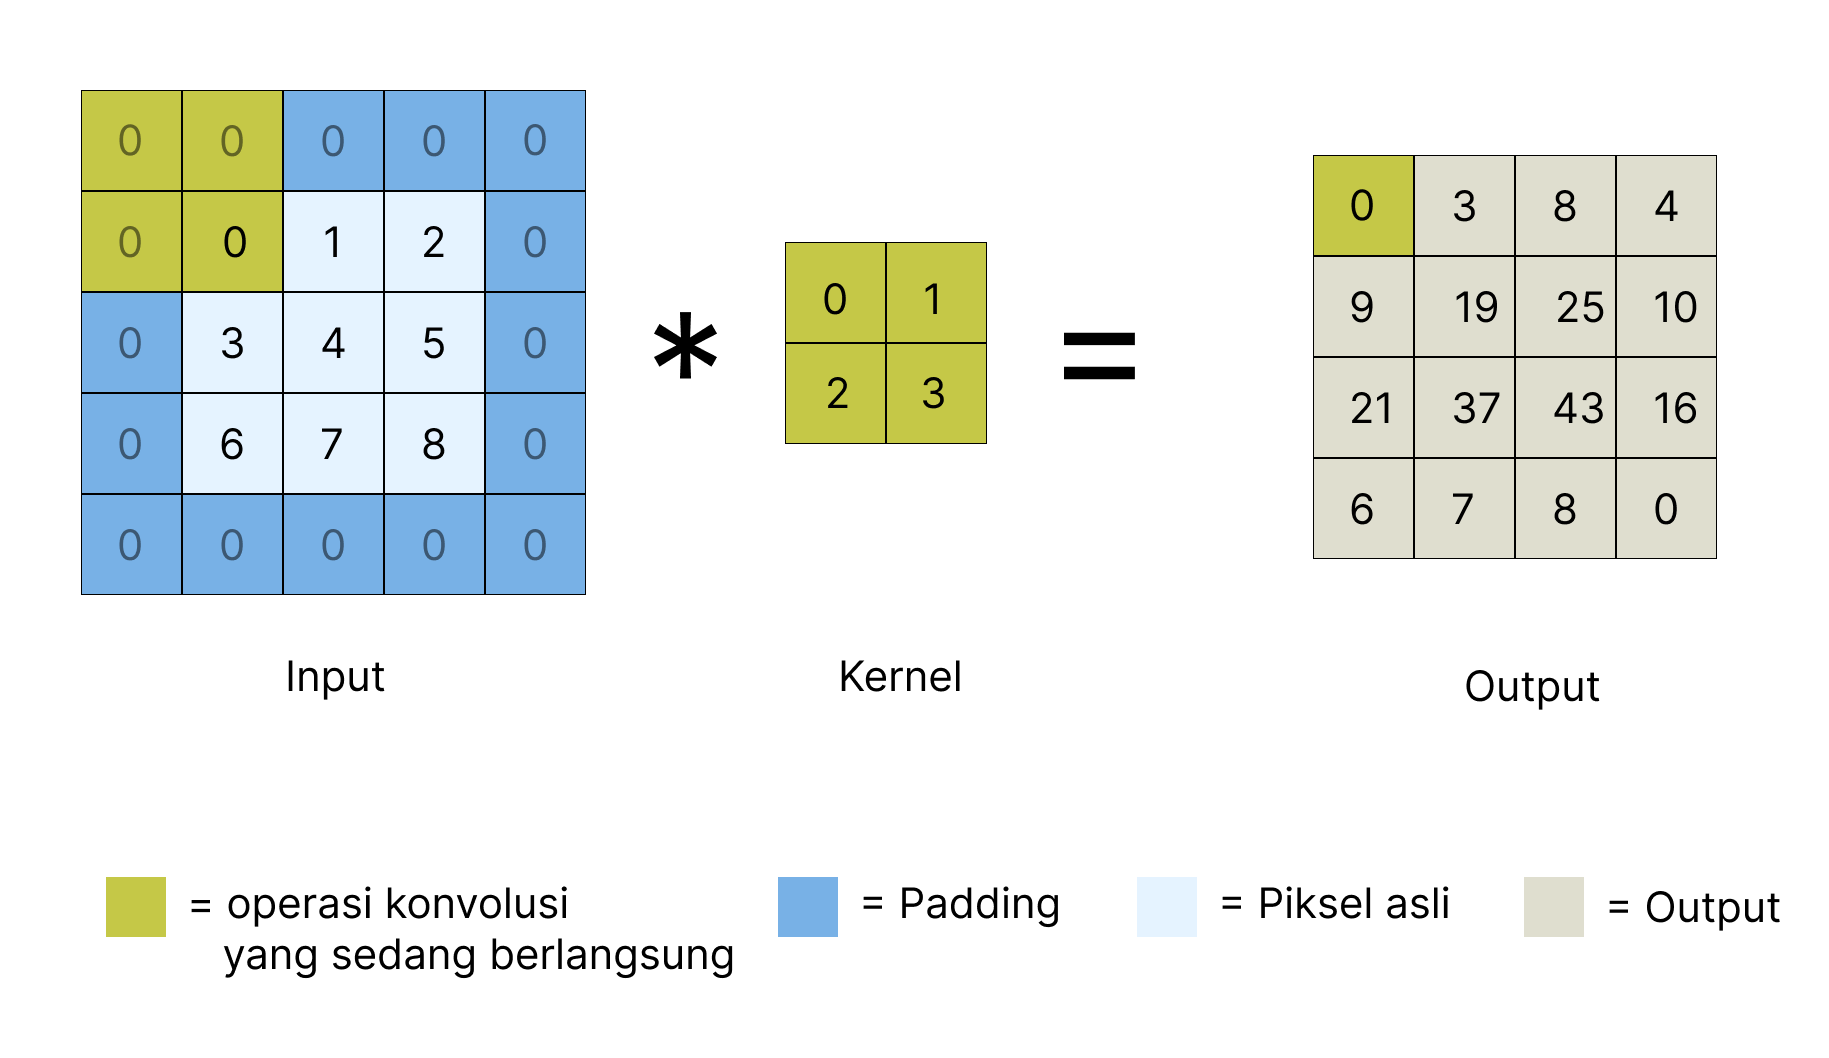
\includegraphics[width=10cm]{gambar/padding.png}
%     \caption{Contoh penggunaan \emph{padding} pada gambar asli ukuran $3 \times 3$.\\ \emph{Sumber: dokumen penulis}}
%     \label{padding}
% \end{figure}

% Secara umum, suatu matriks masukan sebesar $n_h \times n_w$ yang dioperasikan pada kernel konvolusi $k_h \times k_w$ dan kemudian ditambah jumlah baris \emph{padding} $p_h$ (di atas dan di bawah) dan jumlah kolom \emph{padding} $p_w$ (di kiri dan di kanan), maka akan menghasilkan luaran dengan bentuk:
% \begin{equation}
%     \left(n_h - k_h + p_h +1\right) \times \left(n_w - k_w + p_w + 1\right)
% \end{equation}

% \subsection{Lapisan Penyatuan (\emph{Pooling Layer})}
% \emph{Pooling layer} atau lapisan penyatuan berfungsi untuk mengurangi ukuran spasial dari fitur hasil operasi konvolusi dan membantu mengurangi \emph{overfitting} \citep{zocca_spacagna_slater_roelants_2017}. Operasi \emph{pooling} yang paling jamak digunakan adalah \emph{max-pooling}, yang membuat kisi (\emph{grid}) pada tiap potongan fitur dan kemudian mengambil nilai piksel yang paling besar pada tiap kisi dan mengabaikan yang lain. \emph{Pooling layer} tidak menambahkan parameter baru, karena hanya mengekstraksi nilai (yang tertinggi, misalnya) tanpa membutuhkan tambahan bobot atau bias.
% \begin{figure}[h]
%     \centering
%     \includesvg[width=5cm]{max_pooling}
%     \caption{Ilustrasi \emph{max pooling layer} dengan ukuran $2 \times 2$ dan \emph{stride} = 2 dikenakan pada fitur dengan ukuran $4 \times 4$. \emph{Sumber: penulis.} }
%     \label{max_pooling}
% \end{figure}

% \emph{Pooling layer} memiliki dua parameter yaitu ukuran sel dan \emph{stride}. Dapat dirumuskan bentuk luaran dari hasil operasi \emph{pooling layer}. $I$ merupakan masukkan (\emph{input}) atau layer fitur hasil konvolusional, $F$ merupakan ukuran \emph{pooling layer} dan $S$ merupakan \emph{stride} dari \emph{pooling layer}. Indeks $w$ dan $h$ merupakan representasi dari lebar (\emph{width}) dan tinggi (\emph{height}) secara berturut-turut.

% \begin{equation}\label{max_pooling}
% \begin{split}
%     O_w = \frac{(I_w - F_w)}{S_w} + 1\\
%     O_h = \frac{(I_h - F_h)}{S_h} + 1
% \end{split}
% \end{equation}

% Operasi \emph{max pooling} bukanlah satu-satunya operasi penyatuan (\emph{pooling}). Ada beberapa operasi penyatuan lain, misalnya \emph{average pool} yang mengambil nilai rata-rata dari piksel yang dikenai oleh \emph{pooling layer}, atau $L^2$ yang merupakan akar pangkat dari jumlah nilai piksel. Dibandingkan dengan operasi penyatuan yang lain, \emph{max pooling} memiliki peforma yang paling baik karena mereduksi \emph{noise} dengan mengabaikan piksel \emph{noisy} yang nilainya kecil \citep{patel_2020}.

% \subsection{Arsitektur CNN}
% Telah ditinjau bahwa CNN umumnya terdiri dari tiga tipe lapisan: konvolusional, \emph{pooling}, \emph{fully conected} (FC). Bentuk paling umum dari arsitektur CNN adalah tumpukkan dari beberapa pasangan konvolusional-ReLU yang diikuti oleh \emph{pooling layer}, dan kemudian pola ini terus berulang hingga gambar input dipadatkan secara spasial menjadi ukuran yang lebih kecil. Lapisan akhir \emph{fully-connected} menghasilkan luaran yang dikehendaki, misalnya kategori untuk klasifikasi ataupun hasil pada regresi. Dengan kata lain, arsitektur paling umum dari CNN adalah sebagai berikut:

% \begin{equation*}
%     \begin{split}
%         MASUKAN \rightarrow &[[KONVOLUSIONAL \rightarrow RELU]*N \rightarrow POOL]\\
%         &*M \rightarrow [FC \rightarrow RELU]*K \rightarrow FC
%     \end{split}
% \end{equation*}

% dengan $*$ mengindikasikan perulangan (repetisi), dan $POOL$ merupakan langkah \emph{pooling} yang opsional. Jumlah perulangan $N, M, K$ masing-masing lebih dari sama dengan $0$. Biasanya, $N \leq 3$ dan $K < 3$ \citep{zhang2020dive}.

% \subsection{U-Net}\label{sub_unet}
% U-Net pertama kali diperkenalkan oleh Olaf Ronneberger, Philipp Fischer, dan Thomas Brox untuk segmentasi biomedis \citep{DBLP:journals/corr/RonnebergerFB15}, dan kemudian mulai banyak digunakan pada komunitas ML-CFD (\emph{Machine Learning - Computation Fluid Dynamics}) \citep{DBLP:journals/corr/abs-2109-13076}.

% Arsitektur ini menggunakan lapisan konvolusi pada semua lapisannya (\emph{fully convolutional layer}). \cite{DBLP:journals/corr/LongSD14} menunjukkan bahwa \emph{fully convolutional layer} pada segmentasi gambar dapat bekerja dengan lebih efisien dan lebih canggih dari arsitektur lainnya tanpa permesinan (\emph{machinery}) lebih lanjut.

% Model U-Net merupakan modifikasi dari model \emph{fully connected layer} yang awalnya dicetuskan oleh \cite{DBLP:journals/corr/LongSD14}. \cite{DBLP:journals/corr/RonnebergerFB15} memodifikasi dan memperpanjang arsitektur yang ada sehingga dapat bekerja dengan beberapa gambar latih dan menghasilkan segmentasi yang lebih presisi (Gambar \ref{unet}).

% \begin{figure}[h]
%     \centering
%     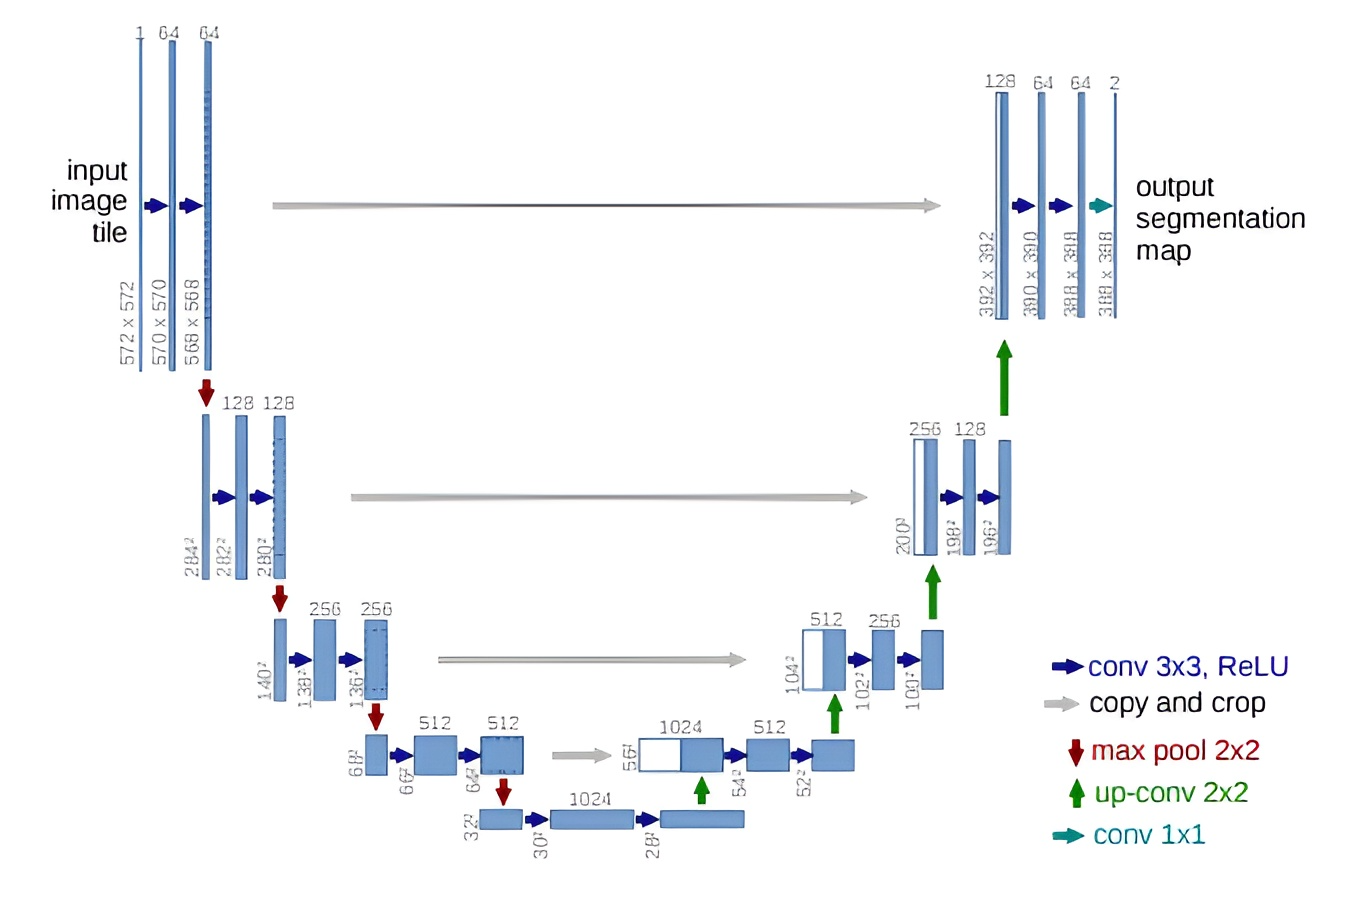
\includegraphics[width=10cm]{gambar/snapedit_1694701272217.png}
%     \caption{Arsitektur U-Net. Tiap kotak biru menunjukkan peta fitur multi kanal. Jumlah kanal ditunjukkan di atas kotak. Ukuran $x-y$ ditunjukkan di tepi kiri bawah kotak. Kotak putih menunjukkan peta fitur yang disalin. Panah menunjukkan operasi-operasi yang terjadi. \emph{Sumber: \citep{DBLP:journals/corr/RonnebergerFB15}}}
%     \label{unet}
% \end{figure}

% Modifikasi yang cukup signifikan terletak pada bagian \emph{upsampling}. Pada bagian ini, masukan yang ukuran spasialnya sudah lebih kecil dari matriks masukan dinaikkan lagi ukurannya (\emph{upsampling}). Pada bagian ini, sejumlah besar kanal fitur memungkinkan jaringan untuk menyebarkan informasi konteks ke lapisan resolusi yang lebih tinggi. Sebagai konsekuensinya, jalur ekspansif (sebelah kanan) kurang lebih simetris dengan jalur kontraksi (sebelah kiri) dan menghasilkan arsitektur berbentuk huruf U. Jaringan ini tidak memiliki \emph{fully connected layer} dan hanya menggunakan bagian yang valid dari setiap luaran konvolusi, yaitu peta segmentasi yang hanya berisi piksel, yang konteks lengkapnya tersedia di dalam gambar masukan. Untuk memprediksi piksel di wilayah perbatasan gambar, konteks yang hilang diekstrapolasi dengan mencerminkan gambar masukan (\emph{crop and copy}).

% Pada arsitektur Gambar \ref{unet}, jalur kontraksi mengikuti arsitektur jaringan konvolusi seperti biasanya. Isinya aplikasi dari lapisan konvolusi $3 \times 3$ (\emph{unpadded convolution}), yang masing-masingnya diikuti oleh fungsi aktivasi ReLU dan operasi \emph{maxpooling} $2 \times 2$ dengan jumlah \emph{stride} 2 untuk \emph{downsampling}. Pada tiap langkah \emph{downsampling}, jumlah kanal fitur diperbanyak 2 kali lipat. Setiap langkah pada jalur ekspansi terdiri dari \emph{upsampling} peta fitur yang diikuti oleh konvolusi $2 \times 2$ (\emph{up-convolution}) yang membagi 2 jumlah kanal fiturnya . Kemudian penggabungan dengan peta fitur terkait yang dipotong dari jalur kontraksi, dan konvolusi $3 \times 3$ yang diikuti oleh fungsi aktivasi ReLU. Penggabungan peta fitur yang terpotong merupakan hal yang perlu dilakukan karena hilangnya batas piksel pada tiap konvolusi \citep{DBLP:journals/corr/RonnebergerFB15}. 

  % \chapter{Metode Penelitian}

\section{Alat dan Bahan}

Perangkat keras yang digunakan dalam penelitian ini adalah berupa komputer dengan
bentuk komputer jinjing (\emph{laptop}) dengan spesifikasi sebagai berikut:

\begin{table}[ht]
  \centering
  \caption{Spesifikasi komputer alat}
  \begin{tabular}{|M{5cm}|M{8cm}|}
    \hline
    \textbf{Komponen} & \textbf{Spesifikasi}                                   \\
    \hline
    Sistem operasi    & Manjaro Linux x86\_64 (Kernel 6.1.55-1-MANJARO)        \\
    \hline
    CPU               & Intel i7-10510U, 4.9 GHz, 4 Cores, 8 Logical Processor \\
    \hline
    GPU               & NVIDIA GeForce MX2500, 2GB                             \\
    \hline
    RAM               & 20 GB                                                  \\
    \hline
    Penyimpanan       & Solid State Drive 480 GB                               \\
    \hline
  \end{tabular}
\end{table}

Kemudian, dalam menjalankan penelitian, penulis menggunakan berbagai perangkat lunak
untuk melakukan \emph{benchmarking}. Adapun perangkat-perangkat lunak tersebut adalah:
\begin{itemize}
  \item Pluto.jl: sebagai \emph{interactive} editor untuk Julia

  \item Bahasa pemrograman Julia: untuk menjalankan metode fisika komputasi

  \item Bahas pemgoraman Python: untuk menjalankan metode fisika komputasi
\end{itemize}

% \section{Bahan}
% Data latih dalam penelitian ini akan menggunakan data sumber distribusi $\rho$
% dari dataset acak yang memiliki rentang [-1,1] yang dibuat menggunakan program PlasmaNet
% \citep{cheng_illarramendi_bauerheim_cuenot_2021}. Dan kemudian dihitung potensial
% listrik $\phi$ menggunakan \emph{solver} Gauss-Seidel untuk plasma berbasis C++
% \citep{lubos_brieda_2019}.

% \section{Alat}
% Perangkat keras yang digunakan peneliti dalam penelitian ini adalah berupa komputer
% dengan bentuk komputer jinjing (\emph{laptop}) dengan spesifikasi sebagai
% berikut:

% \begin{table}[ht]
%   \centering
%   \caption{Spesifikasi komputer alat}
%   \begin{tabular}{|M{3cm}|M{4cm}|}
%     \hline
%     \textbf{Komponen} & \textbf{Spesifikasi}                                                            \\
%     \hline
%     Sistem operasi    & Windows 11 Home                                                                 \\
%     \hline
%     CPU               & AMD Ryzen 5 5600U with Radeon Graphics, 2.30 GHz, 6 Cores, 12 Logical Processor \\
%     \hline
%     GPU               & NVIDIA GeForce RTX 3050, 4GB                                                    \\
%     \hline
%     RAM               & 16 GB                                                                           \\
%     \hline
%     Penyimpanan       & Solid State Drive 512 GB                                                        \\
%     \hline
%   \end{tabular}
% \end{table}

% Kemudian, dalam menjalankan penelitian, penulis menggunakan berbagai perangkat lunak
% untuk membuat data, mengolah data, dan melatih data. Adapun perangkat-perangkat
% lunak tersebut adalah:
% \begin{itemize}
%   \item Visual Studio Code: sebagai pengolah kode

%   \item Google Colab Pro dengan GPU T4: untuk melatih model dengan \emph{graphic
%     processing unit} (GPU)

%   \item Bahasa pemrograman C++: untuk membangun \emph{solver} Gauss-Seidel

%   \item Bahasa pemrograman Python: untuk membangun model dan melatih model \emph{machine
%     learning}
% \end{itemize}

% \section{Prosedur Kerja dan Pengambilan Data}
% Secara garis besar, alur penelitian ini berawal dari pembuatan data latih pasangan
% $\rho$ dan $\phi$, yaitu dengan cara menghitung $\phi$ menggunakan metode Gauss-Seidel
% dari data $\rho$ yang didapatkan dari PlasmaNet, kemudian pemrosesan data agar siap
% untuk jadi data latih, dilanjutkan ke pelatihan model CNN, dan kemudian pengujian
% model CNN. Pada Gambar \ref{flowchart} disajikan alur penelitian dengan model
% diagram alir (\emph{flowchart}).

% \begin{figure}[h!]
%   \label{flowchart}
%   \centering
%   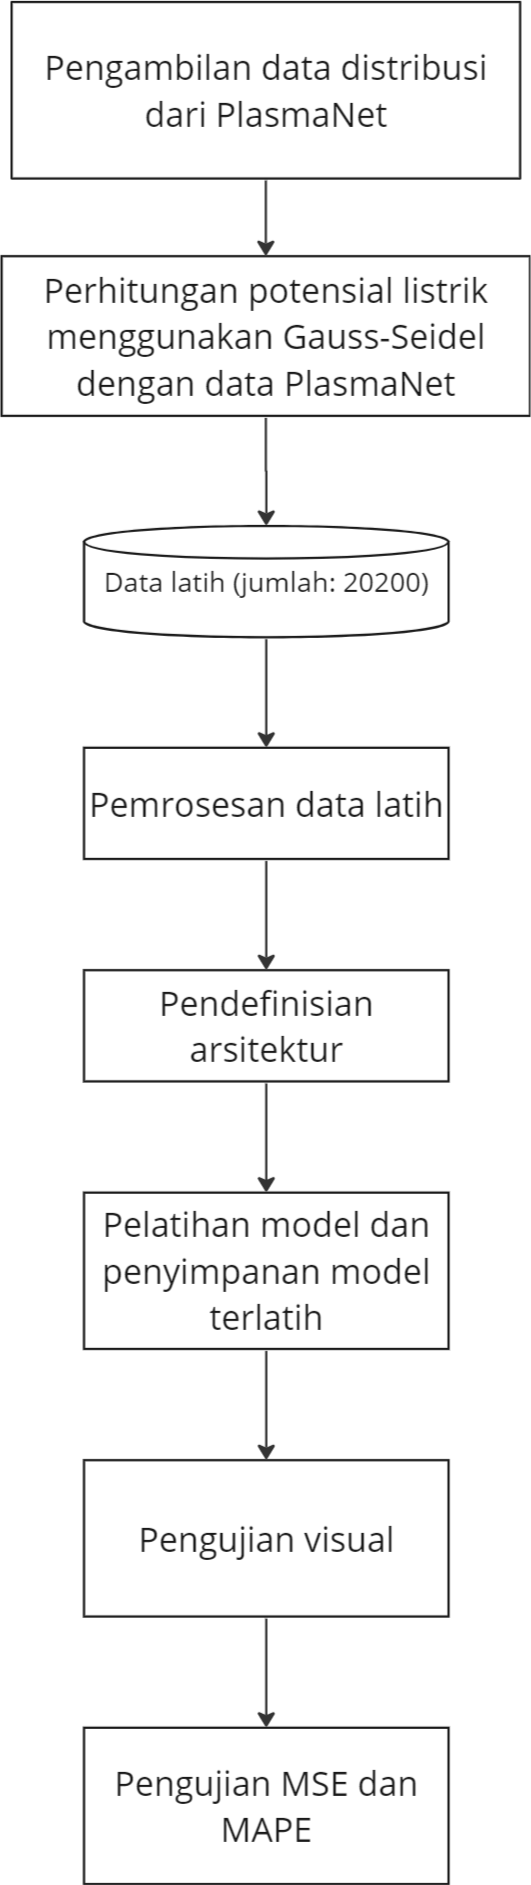
\includegraphics[width=3cm, scale=0.5]{gambar/flowchart2.jpg}
%   \caption{Diagram alir penelitian}
%   \label{flowchart}
% \end{figure}

% \subsection{Pengambilan Data Latih}
% \label{data_latih} Dalam konteks pemelajaran mendalam (\emph{deep learning}),
% data latih berarti pasangan data antara data masukan dan data target. Dan data hasil
% prediksi adalah data uji dan data hasil prediksi. Tahap pertama penelitian ini
% adalah pembuatan data latih. Untuk data masukan, digunakan data distribusi acak
% (sisi kanan pada Persamaan \eqref{poisson umum}) yang dibuat menggunakan program
% PlasmaNet yang dapat dikontrol skala spasialnya. Data distribusi acak memiliki
% nilai yang membentang pada rentang [-1, 1] secara kontinyu. Data ini dibuat pada
% kisi dengan resolusi kasar dengan ukuran $n_{kasar}= [n_{p}/c]$. Dengan $n_{p}$
% adalah jumlah piksel pada tiap sumbu dan $c$ adalah ukuran filter. Kemudian interpolasi
% bikubik membuat bidang random dengan ukuran struktur terkontrol pada kisi target
% \citep{cheng_illarramendi_bauerheim_cuenot_2021}, dengan $c$ adalah ukuran struktur
% minimum. Data distribusi yang diambil pada penelitian ini adalah sebanyak 20.200
% data dengan domain $100 \times 100$.

% \begin{figure}[h!]
%   \centering
%   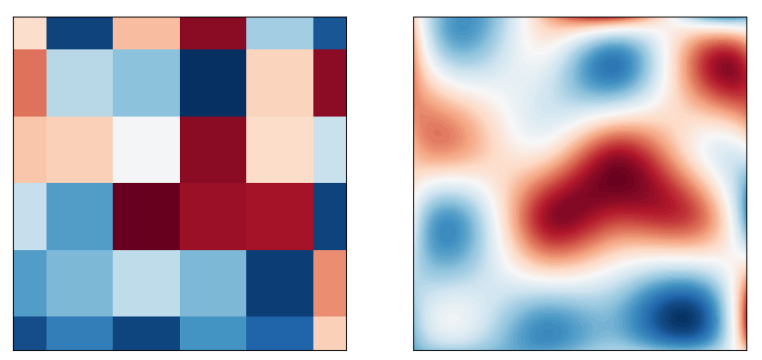
\includegraphics[width=8cm]{gambar/random.png}
%   \caption{Contoh nilai distribusi acak dalam $6 \times 6$ pada kisi kasar (kiri)
%   yang diinterpolasikan pada kisi halus $101 \times 101$ (kanan) \emph{Sumber: \citep{cheng_illarramendi_bauerheim_cuenot_2021}}}
% \end{figure}

% Tahapan pertama yang dilakukan dalam pengambilan data sekaligus dalam penelitian
% ini adalah pembuatan \emph{solver} Gauss-Seidel untuk menghasilkan pasangan
% dataset latih (\emph{training dataset}). Hal pertama yang harus diperhatikan
% dalam pembuatan program pemecah (\emph{solver}) masalah Poisson adalah domain fisis
% yang digunakan. Seperti yang telah disebutkan pada Bab \ref{tipus}, konteks pemecahan
% masalah ini adalah terletak pada koordinat silinder Gambar \ref{domain_silinder}.
% Untuk menjaga karakter kinetik model sepenuhnya, perlu dilakukan pengurangan dimensi
% sistem, membatasi domain menjadi dua dimensi ($r,z$) mengabaikan variasi azimut
% dari besaran yang terlibat (simulasi simetri aksial) \citep{f_taccogna_longo_capitelli_schneider_2005}
% dengan $r \neq 0$. Pemilihan domain ini dikarenakan ada banyak pemanfaatan yang
% dapat digunakan dalam implementasi fisis, salah satunya adalah pendorong Hall (\emph{Hall
% thruster}). Untuk itu, disesuaikanlah domain silinder ini dengan model pendorong
% Hall, adapun model domain pendorong Hall yang digunakan dalam penelitian ini adalah
% SPT-100 karena selain memiliki sejarah keberhasilan yang banyak \citep{braga_miranda_2019},
% perangkat ini juga banyak digunakan sebagai patokan atau percontohan dalam beberapa
% penelitian \citep{Shiferaw2013, f_taccogna_longo_capitelli_schneider_2005, braga_miranda_2019, boeuf_2017}.

% \begin{figure}[h!]
%   \centering
%   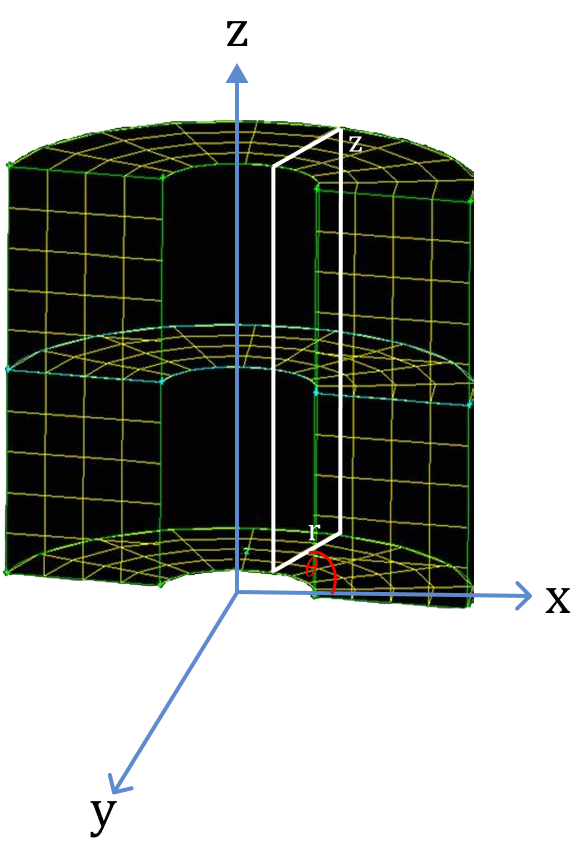
\includegraphics[width=5cm]{gambar/silinder.png}
%   \caption{Tampang lintang koordinat silinder. Penelitian ini menghitung potensial
%   listrik pada koordinat silinder dengan pendekatan simetri aksial, yaitu pada
%   sumbu $r-z$.\emph{ Sumber: \citep{Shiferaw2013} dengan penyesuaian oleh Penulis}}
%   \label{domain_silinder}
% \end{figure}

% Disadur dari \cite{braga_miranda_2019} dan \cite{f_taccogna_longo_capitelli_schneider_2005},
% spesifikasi teknis dan ukuran domain dari model SPT-100 ditampilkan dalam Tabel
% \ref{spt_100}. Domain komputasi numerik pada penelitian ini diilustrasikan dalam
% model 2 dimensi dari SPT-100 yang ditampilkan pada Gambar \ref{spt_100_2d}.

% \begin{table}[h!]
%   \centering
%   \caption{Informasi domain fisis dan teknis pendorong Hall SPT-100 }
%   \label{spt_100}
%   \begin{tabular}{ll}
%     \hline
%     \textbf{Dimensi}             & \textbf{Ukuran} \\
%     \hline
%     Panjang kanal (m)            & 0,025           \\
%     \hline
%     Lebar kanal (m)              & 0,015           \\
%     \hline
%     Panjang kanal keluar (m)     & 0,01            \\
%     \hline
%     Jari-jari silinder dalam (m) & 0,035           \\
%     \hline
%     Jari-jari silinder luar (m)  & 0,05            \\
%     \hline
%     Dorongan (N)                 & 0,08            \\
%     \hline
%   \end{tabular}
% \end{table}

% \begin{figure}[h!]
%   \centering
%   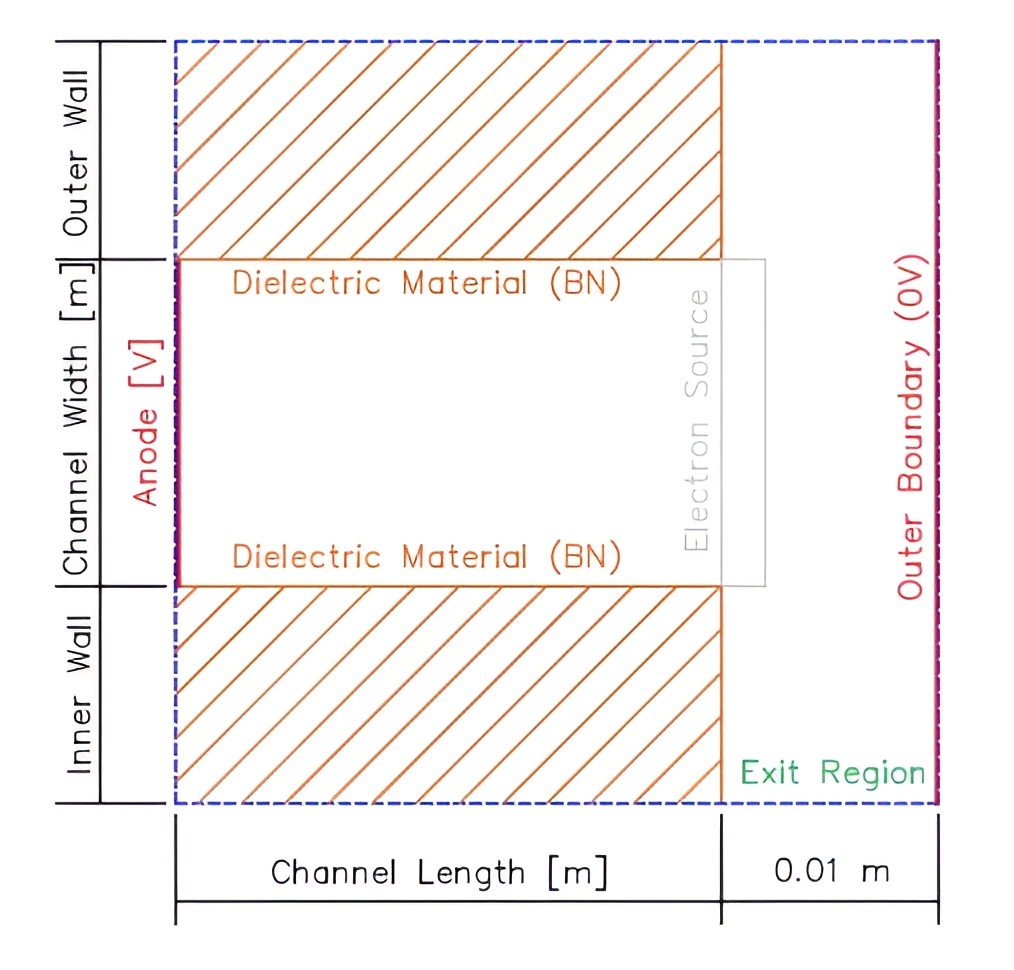
\includegraphics[width=5cm]{gambar/spt_100_2d.png}
%   \caption{Model 2 dimensi dari kanal SPT-100 sebagai domain komputasi numerik. Lebar
%   kanal dimulai dari 0,035 - 0,050 m dan panjang kanal dimulai dari 0,00 - 0,025
%   m. \emph{ Sumber: \citep{braga_miranda_2019}}}
%   \label{spt_100_2d}
% \end{figure}

% \subsubsection{Pengambilan Data Distribusi Pada Program PlasmaNet}

% Data distribusi muatan $\rho$ yang akan digunakan untuk menghitung potensial
% listrik pada pemecah Gauss-Seidel diambil menggunakan program PlasmaNet \citep{cheng_illarramendi_bauerheim_cuenot_2021}.
% Program ini menyediakan pasangan data distribusi partikel secara acak maupun
% distribusi partikel dengan pola sinusoidal dan potensial listriknya. Namun,
% pasangan data tersebut tidak dapat digunakan karena potensial listrik yang
% digunakan mengikuti syarat batas tertentu seperti pada domain komputasi yang
% disebutkan sebelumnya, sehingga hanya akan digunakan data distribusinya ($\rho$)
% saja.

% Dalam pembentukan data distribusi acak, perumusan matematis telah dijelaskan
% sebelumnya pada Subbagian \ref{data_latih}. Hal yang harus diperhatikan untuk pembuatan
% data distribusi acak ini adalah mengenai syarat awal domain serta ukuran spasial
% domain kasar dan halus. Pertama, akan ditinjau mengenai syarat awal yang digunakan
% untuk membentuk distribusi acak.

% \begin{mypythoncode}
%   [Syarat awal pembuatan data distribusi acak di PlasmaNet] xmin: 0.035 xmax: 0.050
%   nnx: 100 ymin: 0.0 ymax: 0.050 nny: 100
% \end{mypythoncode}

% Kode cuplikan Kode 1 dapat dibandingkan dengan Gambar \ref{spt_100_2d}, \texttt{xmin}
% dan \texttt{xmax} merupakan lebar kanal dan \texttt{ymin} dan \texttt{ymax} merupakan
% panjang kanal. Pada bagian ini dilakukan peniruan domain SPT-100 untuk
% distribusi muatan (Gambar \ref{ukuran spt 100}). Kemudian, \texttt{nnx} dan \texttt{nny}
% adalah jumlah piksel untuk tiap sumbu.

% \begin{figure}[h!]
%   \centering
%   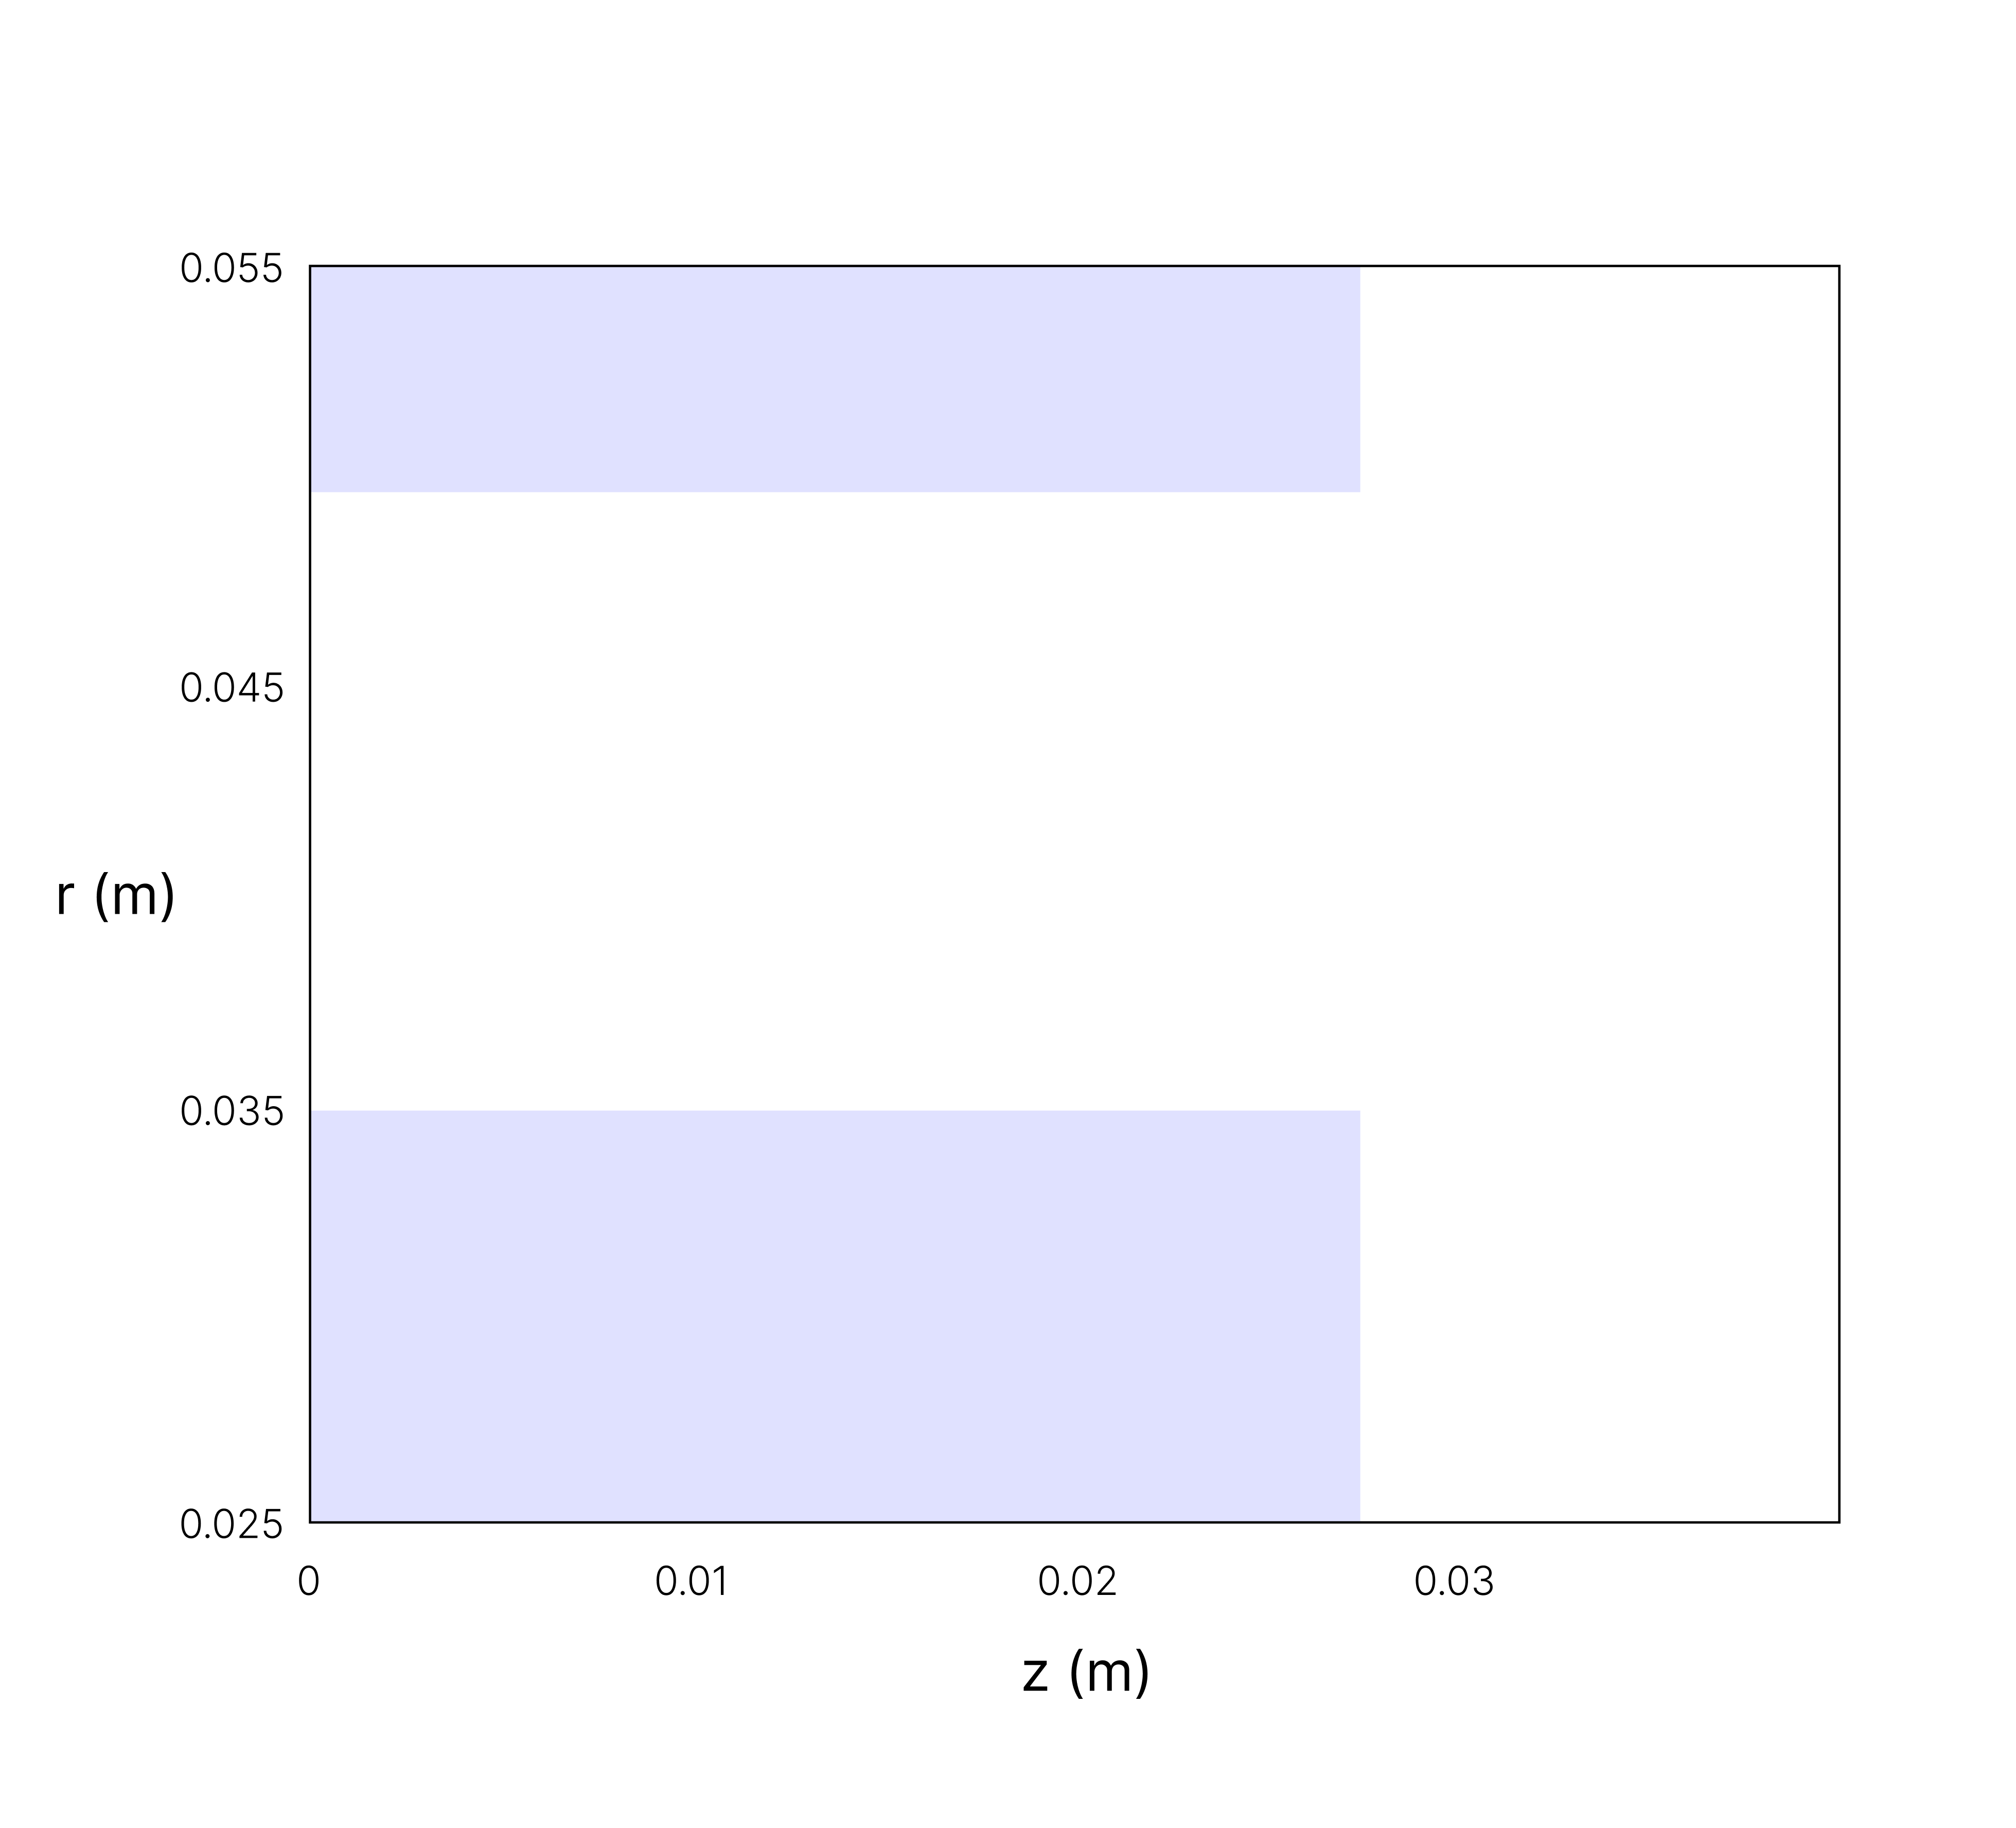
\includegraphics[width=10cm]{gambar/domain spt100 ukuran.png}
%   \caption{Ukuran kanal SPT-100. \emph{ Sumber: Penulis}}
%   \label{ukuran spt 100}
% \end{figure}

% Tahapan selanjutnya dalam pembuatan set data acak adalah memilih parameter $c$ yang
% akan menentukan ukuran struktur minimum pada ukuran domain kasar. Pada
% penelitian ini, akan digunakan domain $100 \times 100$ dan dipilih $c = 16$. Hal
% ini akan membuat domain medan acak dengan ukuran $100/8 \times 100/8 \approx 12$
% dan kemudian akan diinterpolasikan kembali ke ukuran asli $100 \times 100$.

% Setelah didapatkan kumpulan data acak, data tersebut tidak dapat langsung digunakan
% karena setelah dilakukan investigasi singkat pada data-data yang ada, nilai-nilai
% data pada set data distribusi yang dihasilkan sangat kecil (misalnya, banyak
% medan dengan nilai piksel di orde $10^{-34}$) sehingga menyebabkan kesulitan pada
% perhitungan oleh komputer. Sehingga tahapan selanjutnya adalah peningkatan (\textit{scale-up}).
% Upaya peningkatan nilai $\rho$ untuk seluruh jumlah dataset (\texttt{len(rho)}) dilakukan
% dengan cara sebagai berikut:

% \begin{mypythoncode}
%   [Kode cuplikan peningkatan nilai rho] a = len(rho) for i in range (a): rho_max
%   = np.max(rho[i]) rho_min = abs(np.min(rho[i]))

%   if rho_max > rho_min: c = 1/rho_max else: c = 1/rho_min

%   rho[i] = rho[i]*c
% \end{mypythoncode}

% Pada kode tersebut, dicari nilai ekstrim mutlak tertinggi pada tiap medan, dan
% kemudian nilai ekstrim mutlak tersebut digunakan sebagai nilai pembagi di masing-masing
% domain.

% \subsubsection{Syarat Awal dari \textit{Solver} Gauss-Seidel}

% Setelah data distribusi partikel siap, akan dilanjutkan dengan pemecahan masalah
% menggunakan metode Gauss-Seidel. Pada subbab ini dan subbab selanjutnya, akan
% dibahas mengenai syarat awal dan algoritma dari \textit{solver} Gauss-Seidel yang
% digunakan.

% Untuk membangun \textit{solver} perhitungan potensial listrik menggunakan metode
% Gauss-Seidel ini, digunakan bahasa pemrograman C++. Bahasa pemrograman C++
% dipilih pertama-tama karena bahasa ini berkali-kali lipat lebih cepat
% dibandingkan Python, walaupun Python memiliki pustaka (\textit{library}) yang
% cukup bagus dan dapat mengoptimasi kerja komputasi, semisal Numpy \citep{lubos_brieda_2019}.
% Selain itu, Python memiliki kekurangan dalam tipe variabel yang dapat memicu
% \textit{bugs}, terlebih khusus saat pembedaan variabel \textit{integer} dan \textit{floating
% point}. Dari segi pustaka, ada banyak pustaka saintifik yang diimplementasikan
% menggunakan C++ tanpa pembungkus (\textit{wrappers}) pihak ketiga.

% Syarat awal pada \textit{solver} ini didefinisikan dalam sebuah \textit{header
% file}. Dalam \textit{header file} ini berisi konstanta yang digunakan dan juga tebakan
% awal Gauss-Seidel. Pada penelitian ini digunakan satu konstanta yaitu
% $\epsilon_{0} = 8.8541878 \times 10^{-12}$ \citep{lubos_brieda_2019}. Dan untuk
% tebakan awal, digunakan nilai tebakan awal = 0 untuk seluruh piksel pada matriks
% tebakan awal.

% \subsubsection{Algoritma \textit{Solver} Gauss-Seidel}

% Pada subbagian ini akan dibahas mengenai implementasi dari Subbagian
% \ref{gauss_seidel_silinder} pada \textit{solver} Gauss-Seidel menggunakan bahasa
% pemrograman C++. Secara umum, \textit{solver} ini akan menjalankan 2 file. Yang pertama
% adalah file untuk mendefinisikan algoritma dari Gauss-Seidel sekaligus untuk menuliskan
% hasil (dalam penelitian ini file tersebut diberi nama \texttt{Potential.cpp} (Lampiran
% \ref{kode_potential_cpp})) dan file yang kedua adalah untuk memberikan syarat
% awal atau konteks besaran domain dan juga pada file ini terjadi pemanggilan
% fungsi-fungsi yang didefinisikan pada \texttt{Potential.cpp} beserta pengisian nilainya.
% Nama file ini pada penelitian ini adalah \texttt{main.cpp} (Lampiran
% \ref{kode_main_cpp}).

% Tahap paling awal pada \texttt{Potential.cpp} adalah pemanggilan \textit{header
% file} dan pustaka yang dibutuhkan. Setelah itu, dilakukan penginisialisasian menggunakan
% \textit{constructor} \texttt{Solver} untuk matriks masukan dan matriks luaran.
% Kemudian, akan didefinisikan besaran-besaran lain yang merupakan jarak domain pada
% fungsi \texttt{setextents} dan untuk jumlah iterasi maksimal dan toleransi ralat
% diatur pada fungsi \texttt{setParam}.

% Setelah semua kondisi diatur, masuk pada perhitungan iterasi pada fungsi \texttt{writeSolveGS}.
% Di sini, argumen yang digunakan adalah \texttt{filename}, \texttt{reshape\_\texttt{\-}rows},
% \texttt{reshape\_cols}, yang nilai argumennya semuanya terletak pada \texttt{main.cpp}.
% Berikut adalah \textit{pseudocode} dari algoritma implementasi perhitungan Gauss-Seidel:
% \begin{lstlisting}[breaklines=true, breakatwhitespace=true]
% DEFINISIKAN variabel: idz, idr, idz2 (idz pangkat dua), idr2 (idr pangkat dua), crz
% SET L2 ke 0
% SET converged ke False

% FOR iterasi < nilai iterasi maksimal:
%     iterasi ditambah 1
%     FOR i < jumlah baris keseluruhan data:
%         i ditambah 1
%         FOR j < jumlah kolom:
%             j ditambah 1
%             IF i = 0 ATAU i kelipatan 100: #syarat batas paling atas
%                 CONTINUE
%             ELSE IF i modulo 100 = 99: #syarat batas paling bawah
%                 phi(i,j) = phi(i-1, j)
%             ELSE IF j = 0: #syarat batas paling kiri
%                 CONTINUE
%             ELSE IF j = 99: #syarat batas paling kanan
%                 CONTINUE
%             ELSE: #selain di syarat batas (interiornya)
%                 hitung crj
%                 hitung phi baru menggunakan rho dari file yang ada
%                 lanjutkan dengan SOR

%     IF iterasi kelipatan 100:
%         hitung L2 antara 2 iterasi

%         IF L2 < nilai toleransi
%             perhitungan konvergen atau converged = True
%             BREAK

%     IF tidak konvergen:
%         tampilkan teks: "Gauss seidel standar gagal konvergen, L2=", masukkan nilai L2

%     #penulisan hasil phi pada file csv
%     FOR i < jumlah baris keseluruhan data:
%         i ditambah 1
%         FOR j < jumlah kolom:
%             j ditambah 1
%             IF j pada indeks kolom terakhir:
%                 tulis phi(i,j) diikuti pindah baris
%             ELSE
%                 tulis phi(i,j) diikuti tanda koma (,)
% \end{lstlisting}

% Variabel-variabel yang didefinisikan di awal merupakan variabel yang akan
% digunakan pada perhitungan interior domain, yang detail perhitungannya dapat dilihat
% pada kode sumber. Untuk syarat batas pada atas, kiri, dan kanan, diimplementasikan
% syarat batas Dirichlet nol, sedangkan pada batas paling bawah diterapkan syarat
% batas Neumann. Pada perhitungan Gauss-Seidel di interior menggunakan implementasi
% penyelesaian persamaan Poisson menggunakanm metode Gauss-Seidel seperti pada Subbagian
% \ref{gauss_seidel_silinder} dan parameter SOR 1,4 untuk mempercepat konvergensi seperti
% pada \cite{lubos_brieda_2019}.

% Setiap 100 iterasi, dihitung nilai metrik L2 untuk menentukan nilai ralatnya. Nilai
% L2 ini merupakan nilai rerata ralat dari seluruh piksel iterasi tersebut dengan iterasi
% sebelumnya. Apabila nilai setelah iterasi ke-100 nilai L2 sudah di bawah nilai
% toleransi, maka iterasi pada medan tersebut dihentikan. Namun apabila belum,iterasi
% dilanjutkan pada iterasi kelipatan 100 lainnya dan diperiksa lagi apakah sudah
% di bawah nilai toleransi. Apabila nilai L2 pada medan tersebut belum sampai di bawah
% nilai toleransi sampai pada jumlah iterasi maksimal, maka iterasi pada medan
% tersebut dianggap gagal dan program akan mengeluarkan pesan galat "Gauss seidel standar
% gagal konvergen, L2=" diikuti dengan nilai L2 terakhir.

% Untuk memanggil fungsi-fungsi yang ada pada program Lampiran
% \ref{kode_potential_cpp}, digunakan program lain, yaitu program pada Lampiran
% \ref{kode_main_cpp}. Dalam Lampiran \ref{kode_main_cpp} ditampilkan contoh kasus
% saat program menghitung 2.000 data. Variabel \texttt{nz} adalah jumlah baris keseluruhan
% data, sehingga nilainya $2.000 \times 100 = 200.000$, dan variabel \texttt{nr}
% adalah jumlah kolom domain, yaitu 100.

% Variabel \texttt{totalData} merupakan jumlah seluruh piksel yang dilibatkan dalam
% perhitungan ini. File \textit{comma separated value} (CSV) dari data distribusi yang
% digunakan dipanggil pada variabel \texttt{rho} yang kemudian diubah bentuknya
% menjadi $nz \times nr$. Untuk parameter domain SPT-100 (Tabel \ref{spt_100}) didefinisikan
% pada pemanggilan fungsi \texttt{setextents}. Jumlah iterasi maksimal yang digunakan
% pada perhitungan ini sebesar 100.000 dan nilai toleransi yang diizinkan adalah 0,01.
% Kedua parameter tersebut didefinisikan pada fungsi \texttt{setParam}. Tidak ada referensi
% baku mengenai nilai maksimal iterasi dan nilai ralat yang digunakan. Pada
% \cite{lubos_brieda_2019}, untuk ukuran domain $21 \times 21 \times 21$ sebanyak 1
% data, digunakan nilai iterasi maksimal 5000 dan nilai toleransi 0. Berdasarkan
% acuan ini, dicoba nilai iterasi maksimal dan nilai toleransi ralat yang wajar,
% dapat diandalkan, serta realtif cepat untuk domain 100 $\times$ 100 dengan 2.000
% data (digunakan jumlah 2.000 data dalam sekali perhitungan untuk mencegah agar
% jangan sampai terjadi kerusakan pada perangkat keras karena durasi \textit{runtime}
% yang terlalu lama dan penggunaan memori yang terlalu besar), maka digunakan jumlah
% iterasi maksimal sebanyak 100.000 dan toleransi ralat sebesar 0,01.

% Selain data latih, untuk melatih model yang ada, dibutuhkan data validasi (\emph{validation
% data}) untuk melihat peforma dari model tanpa bias dari data latih \citep{jason_brownlee_2017}.
% Dalam penelitian ini, data validasi diambil sebanyak 25\% dari total data latih.

% \subsection{Pengambilan Data Uji}
% Setelah model didapatkan untuk dilatih, kemudian model diuji dengan data lain
% yang tidak pernah dilihat sebelumnya oleh model. Data tersebut sebagian merupakan
% kumpulan data dengan distribusi acak dan sebagian merupakan data dengan distribusi
% partikel mengikuti aturan Gaussian (Persamaan \eqref{gaussian}):

% \begin{equation}
%   \label{gaussian}f(x,y) = A \enspace exp \left(-\left(\frac{(x-x_{0})^{2}}{2
%   \sigma^{2}_{X}}+ \frac{(y-y_{0})^{2}}{2 \sigma^{2}_{Y}}\right)\right)
% \end{equation}

% Dengan $A$ adalah amplitudo, $x_{0}$ dan $y_{0}$ merupakan koordinat titik pusat,
% dan $\sigma_{x}$, $\sigma_{y}$ merupakan standar deviasi pada sumbu $x$ dan $y$.

% \subsection{Pemrosesan data}
% Salah satu keuntungan terbesar penggunaan jaringan saraf buatan adalah, tidak perlu
% dilakukan \emph{feature engineering}. Lapisan tersembunyi (\emph{hidden layer})
% yang akan mempelajar fitur-fitur dari data yang diberikan \citep{denny2015}.
% Sehingga tidak diperlukan pemrosesan data yang membutuhkan usaha besar.

% Pemrosesan data yang dilakukan adalah pengubahan dimensi bentuk dan normalisasi.
% Perubahan bentuk dalam hal ini adalah pengubahan data-data menjadi masing-masing
% bentuk matriks persegi dalam satu kolom. Kemudian dilakukan normalisasi untuk
% mentransformasi fitur menjadi skala yang mirip, sehingga meningkatkan peforma dan
% stabilitas pelatihan model \citep{google_2022}. Normalisasi yang dilakukan adalah
% penskalaan (\emph{scaling}). Penskalaan berarti mengubah nilai titik data dari rentang
% aslinya ke rentang standar (biasanya 0 sampai 1 atau -1 sampai 1).

% \subsection{Pendefinisian arsitektur}

% Pendefinisian arsitektur dilakukan sesuai dengan bentuk data yang masuk dan bentuk
% data luaran yang dikehendaki. Penambahan regulator, \emph{pooling layer}, dan \emph{padding}
% juga dilakukan di sini. Tidak ada patokan yang baku mengenai bentuk arsitektur dan
% \emph{hyperparameter} yang akan digunakan. Penentuannya akan dilakukan dengan metode
% \emph{trial and error}.

% \subsection{Pelatihan model}
% Model atau arsitektur yang sudah ada kemudian dilatih atau di-\emph{fitting} dengan
% data latih yang disediakan dan divalidasi dengan data validasi yang terpisah dari
% data latih. Pada proses pelatihan ini menggunakan fungsi ralat MSE \ref{mse}, dengan
% \emph{batch size} 32, 200 \emph{epoch}. Kemudian dengan menggunakan pengoptimasi
% ADAM \citep{kingma2017adam} dengan laju pemelajaran awal (\emph{inital learning
% rate}) = 0.001 dan diterapkan penjadwalan laju pemelajaran dengan langkah peluruhan
% (\emph{decay steps}) = 10000 dan laju peluruhan (\emph{decay rate}) = 0.9.

% Sembari dilatih, semua model dari tiap \emph{epoch} disimpan dalam bentuk file h5
% dan kemudian dipilih model yang paling baik dengan cara melihat kurva pemelajaran
% yang muncul setelah model terlatih seutuhnya. Kriteria model yang paling baik
% adalah model dengan \emph{validation loss} paling rendah dan berada di bawah atau
% sama atau hampir sama dari \emph{training validatrion} (\emph{goodfit}).

% \subsection{Evaluasi dan pengujian}
% Masuk ke tahap evaluasi dan pengujian, pertama akan dimuat data uji yang sudah
% dibuat sebelumnya. Kemudian, muat model \emph{epoch} ke-100, \emph{epoch} ke-200,
% dan \emph{epoch} dengan model paling baik. Kemudian lakukan prediksi dengan data
% distribusi $\rho_{uji}$ untuk tiap model.

% Selanjutnya, akan dibandingkan $\phi_{pred}$ yang merupakan hasil prediksi model
% dan $\phi_{uji}$. Sebelum dilakukan pembandingan, data $\phi_{uji}$ dilakukan normalisasi
% terlebih dahulu. Uji yang pertama adalah uji visual pada matriks yang diuji. Di sini
% akan dilihat secara visual seberapa mirip antara $\phi_{uji}$ dan $\phi_{pred}$.

% Selanjutnya akan dipilih beberapa piksel secara acak untuk diketahui nilainya,
% baik pada $\phi_{uji}$ maupun $\phi_{pred}$. Data piksel tersebut kemudian dibandingkan
% dengan cara dihitung MSE dan MAPE-nya.

% Uji selanjutnya adalah pengujian menggunakan MAPE. Akan dipilih nilai-nilai yang
% jauh dari nol. Kemudian dihitung MAPE dari nilai tersebut. Dari pengujian
% tersebut ditentukan nilai MAPE tertinggi, MAPE terendah, dan rata-rata dari
% keseluruhan MAPE.

% =========================

% \subsection{Rencana Kegiatan Penelitian}
% % Please add the following required packages to your document preamble:
% % \usepackage{lscape}
% % \usepackage{longtable}
% % Note: It may be necessary to compile the document several times to get a multi-page table to line up properly
% \begin{landscape}
% \begin{longtable}[c]{|l|l|l|l|l|l|l|l|l|l|l|l|}
% \caption{Tabel Rencana Kegiatan Desember 2022 -- September 2023}
% \label{des_sep}\\
% \hline
% No. & Kegiatan                    & Desember   & Januari    & Februari   & Maret      & April      & Mei        & Juni       & Juli       & Agustus    & September \\ \hline
% \endfirsthead
% %
% \multicolumn{12}{c}%
% {{\bfseries Table \thetable\ continued from previous page}} \\
% \hline
% No. & Kegiatan                    & Desember   & Januari    & Februari   & Maret      & April      & Mei        & Juni       & Juli       & Agustus    & September \\ \hline
% \endhead
% %
% 1 &
%   \begin{tabular}[c]{@{}l@{}}Pembelajaran \\ machine learning\end{tabular} &
%   \checkmark &
%   \checkmark &
%   \checkmark &
%   \checkmark &
%   \checkmark &
%   \checkmark &
%    &
%    &
%    &
%    \\ \hline
% 2   & Pemantapan isu              & \checkmark & \checkmark & \checkmark & \checkmark & \checkmark & \checkmark &            &            &            &           \\ \hline
% 3 &
%   \begin{tabular}[c]{@{}l@{}}Prototyping menggunakan \\ dimensi yang lebih rendah\end{tabular} &
%   \checkmark &
%   \checkmark &
%   \checkmark &
%   \checkmark &
%   \checkmark &
%   \checkmark &
%    &
%    &
%    &
%    \\ \hline
% 4   & Penulisan proposal          &            &            &            &            &            & \checkmark &            &            &            &           \\ \hline
% 5   & Pengambilan data            &            &            &            &            &            & \checkmark & \checkmark & \checkmark & \checkmark &           \\ \hline
% 6   & Prototyping arsitektur UNet &            &            &            &            &            &            &            &            & \checkmark &           \\ \hline
% 7   & Penelitian  arsitektur      &            &            &            &            &            &            &            &            & \checkmark &           \\ \hline
% 8 &
%   \begin{tabular}[c]{@{}l@{}}Penulisan hasil dan\\ pembahasan\end{tabular} &
%    &
%    &
%    &
%    &
%    &
%    &
%    &
%    &
%   \checkmark &
%   \checkmark \\ \hline
% \end{longtable}
% \end{landscape}
  \singlespacing
\bibliography{skripsi.bib}
\onehalfspacing
  %-----------------------------------------------------------------
  %Disini akhir masukan Bab
  %-----------------------------------------------------------------

  %-----------------------------------------------------------------
  %Disini awal masukan untuk Daftar Pustaka (ISI SESUAI DENGAN DATA ANDA!)
  %-----------------------------------------------------------------
  %-----------------------------------------------------------------
  %-----------------------------------------------------------------

  %-----------------------------------------------------------------
  %Disini awal masukan untuk Lampiran (JIKA DIPERLUKAN)
  %-----------------------------------------------------------------
  %\appendix
  %\chapter{SKRIP PROGRAM JAVA}
  %\lstset{language=java, frame=single}
  %\lstset{numbers=left, numberstyle=\tiny, stepnumber=1, numbersep=5pt, basicstyle=\footnotesize}
  %\lstset{frame=shadowbox, xleftmargin=6pt, xrightmargin=8pt, rulesepcolor=\color{black}}
  %\lstset{keywordstyle=\color{blue},breaklines=true, breakindent=27pt}
  %\lstinputlisting{Main.java}
  %
  %
  %\chapter{TABEL KODE ASCII}
  %\begin{figure}[H]
  %\centering
  %\includegraphics[width=14cm]{ASCIIreguler}
  %\end{figure}
  %%-----------------------------------------------------------------
  %%-----------------------------------------------------------------
\end{document}